\section*{Introduction}\index{Amphiesmenoptera}
\textbf{Amphiesmenoptera} comprises two familiar orders, Lepidoptera (moths and butterflies; covered in section \ref{Lepidoptera}) and Trichoptera (caddisflies; section \ref{Trichoptera}), whose close relationship is uncontroversial. To open this unit we'll discuss the evolutionary significance of two characteristics shared by these insects: silk production (from the labium) and hairy bodies, including wings.

\section{Lepidoptera}\label{Lepidoptera}\index{Lepidoptera}

\noindent{}\textbf{Lepidoptera} is one of the ``big four'' orders of insects, and with \textgreater157,000 described species \citep{van2011order} and at least 350,000, probably many more, remaining to be described. These insects are commonly referred to as moths and butterflies, and they remain one of the most recognizable groups of insects. Family-level diagnostics can be difficult, however, given that many characters are obscured by flattened setae called \latinword{scales}. The vast majority of species feed on plants as larvae (caterpillars), and adults live on liquid diets, imbibed through coiled, siphon-like mouthparts (\latinword{proboscis}, formed from the \latinword{galeae}). The hind wings of most species (\textit{i.e.}, the taxon Heteroneura) are different in shape (usually shorter and more rounded) and venation from the fore wings.

\subsection{Zeugloptera (mandibulate moths)}\index{Zeugloptera}
Moths in suborder Zeugloptera have functional mandibles and no proboscis. These moths are classified in a single family, \textbf{Micropterigidae} (mandibulate archaic moths; figure \ref{fig:micropterigid}), and one rare species occurs in the eastern USA. Larvae feed primarily on fungi, mosses, and liverworts. Adults can be found on flowers, where they feed on pollen. \index{Micropterigidae}

\begin{figure}[ht!]
  \centering
    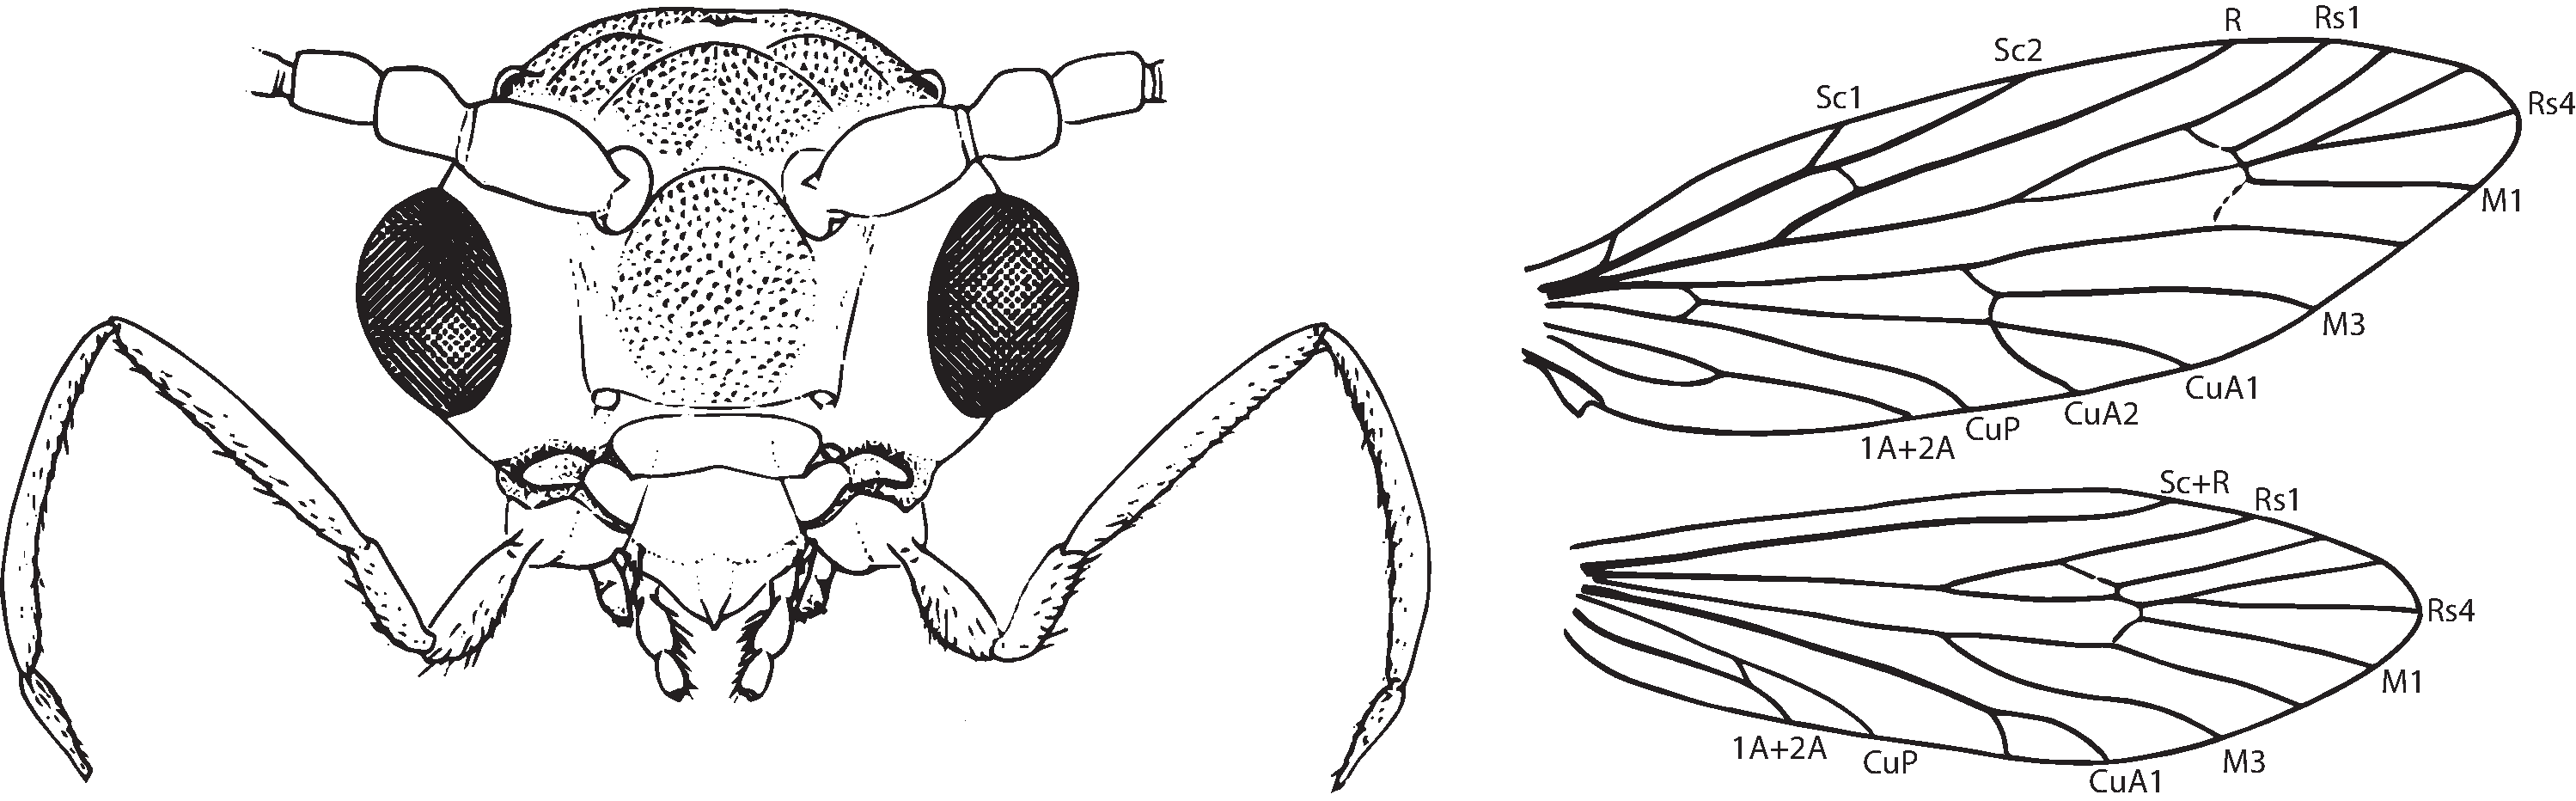
\includegraphics[width=0.7\textwidth]{amphiesmenoptera/Micropterigidae.pdf}
  \caption{Micropterigidae head and wings \citep[modified from][Fig. 13,16]{davis2012review}}
  \label{fig:micropterigid}
\end{figure}

\subsection{Non-dytrisian Lepidoptera (``Monotrysia'')}\index{Monotrysia}
Note that several families in North America have a single opening (\latinword{cloaca}) at the apex of their abdomens, the \latinword{monotrysian} phenotype, through which copulation, oviposition, and defecation occur. We will cover one monotrysian family, Nepticulidae, that is frequently encountered in the northeast.%Incurvariidae on maples!!! Adelidae also and Yucca moths (Prodoxidae)

\subsubsection{Nepticulidae (serpentine leafminer moths)}\index{Nepticulidae}
\noindent{}\textit{Diagnostic characters:} Wingspan 3.5--10 mm, among the very smallest of moths; usually black and white, with a metallic band or gold speckles; antennae with an eye cap (figure \ref{fig:nepticulid1}); maxillary palps well developed, long and folded; wing shape lanceolate; fore wing with relatively simple, branching venation (figure \ref{fig:nepticulid2}).\vspace{3mm}

\noindent{}\textit{Natural history:} Larvae make thin, winding mines on the leaves of trees and shrubs. There are roughly 800 described species.\vspace{3mm}

\begin{figure}[ht!]
    \centering
    \begin{subfigure}[ht!]{0.42\textwidth}
        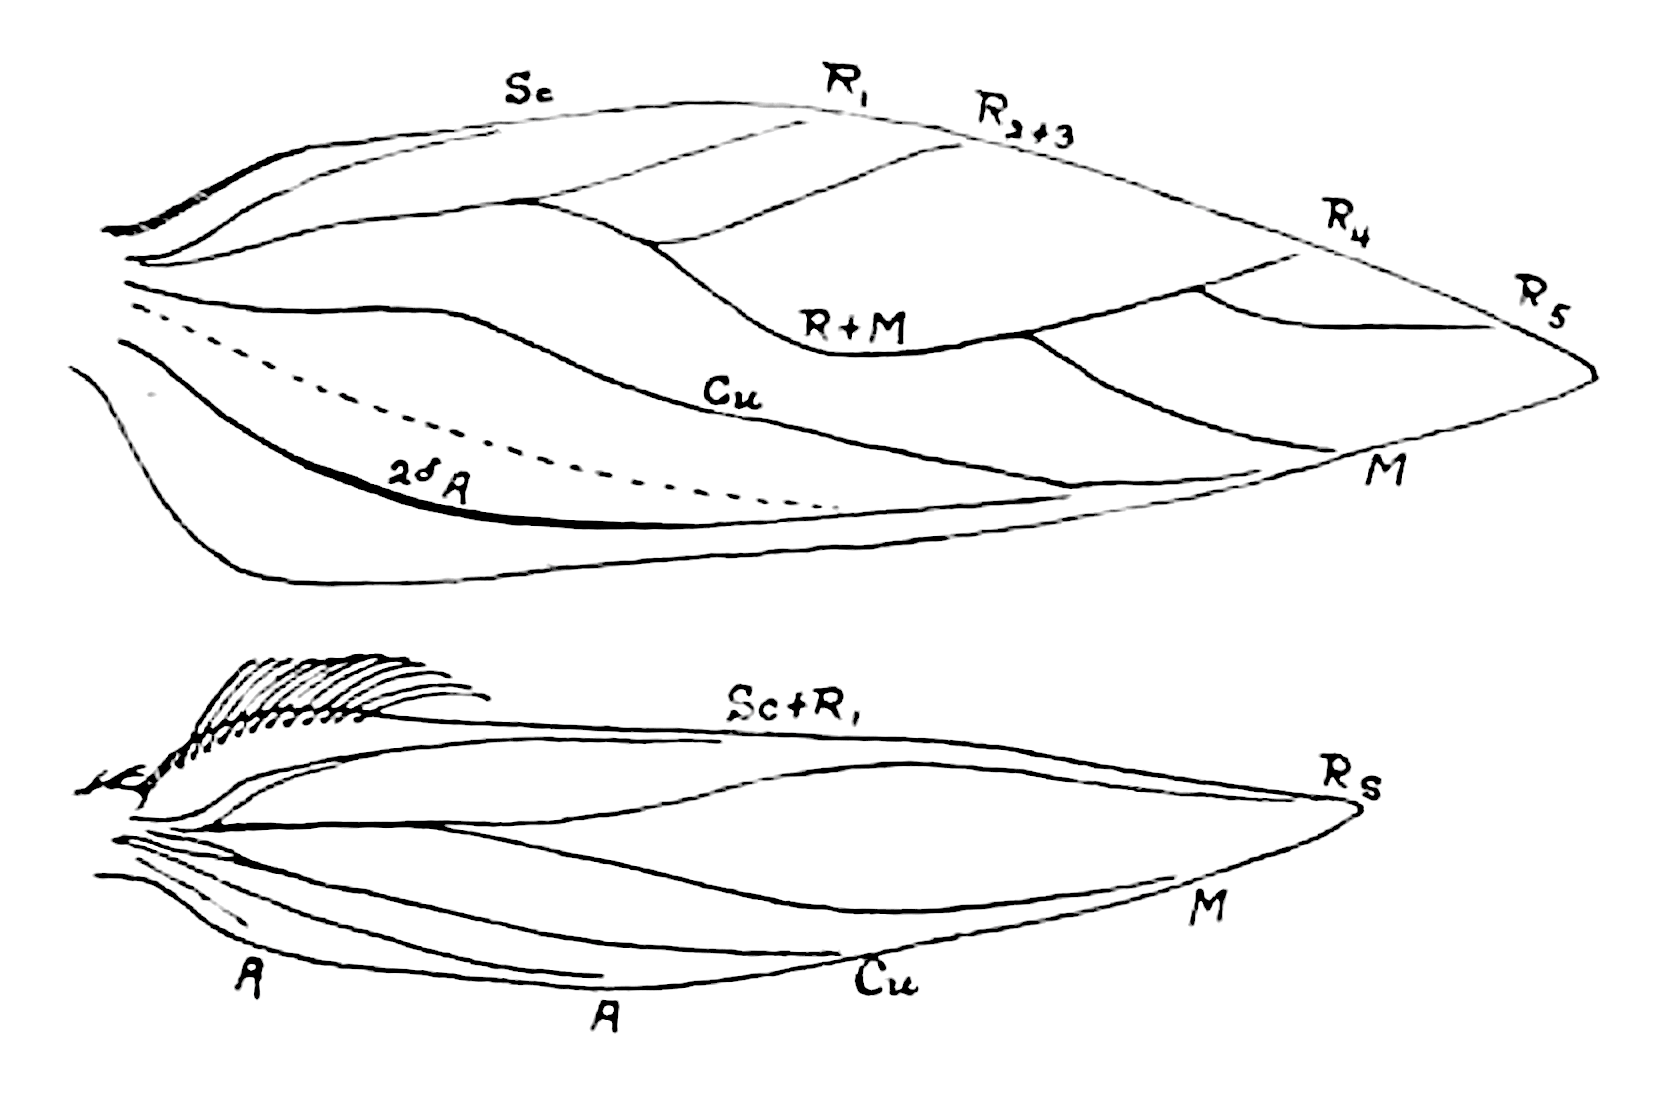
\includegraphics[width=\textwidth]{amphiesmenoptera/NepticulidWings}
        \caption{}
        \label{fig:nepticulid2}
    \end{subfigure}
    \hfill
    \begin{subfigure}[ht!]{0.45\textwidth}
        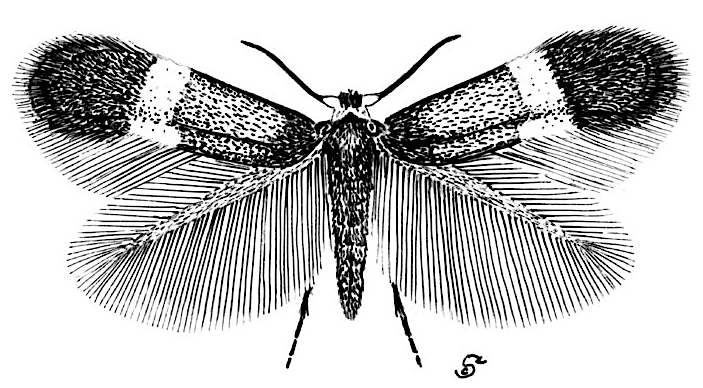
\includegraphics[width=\textwidth]{amphiesmenoptera/nepticulidHabitus}
        \caption{}
        \label{fig:nepticulid1}
    \end{subfigure}
    \caption{Nepticulidae. \textbf{(a)} Wings \citep[][Fig. 1]{braun1917nepticulids}; \textbf{(b)} Dorsal habitus, illustration (CC BY 3.0) by Csaba Szaboky (Image 1296001 at \url{https://www.forestryimages.org/})}\label{fig:nepticulids}
\end{figure}

\subsection{Dytrisia}\index{Dytrisia}
The remaining lepidopterans, \textgreater98\% of all species, are classified in an unranked (sometimes a ``division''), monophyletic taxon called Ditrysia. These insects have separate openings for copulation, oviposition, and defecation.

\subsubsection{Gracillariidae (blotch leafminer moths)}\index{Gracillariidae}
\noindent{}\textit{Diagnostic characters:} Minute to small in size (wingspan 5--20 mm); often brightly colored or metallic; maxillary palps usually absent; proboscis bare; wing venation reduced and elongate along proximal-distal axis, wing fringe long (figure \ref{fig:gracill2}); hind wing lanceolate.\vspace{3mm}

\noindent{}\textit{Natural history:} Most species develop as leaf miners on trees. Some species exhibit hypermetamorphosis, with early instars (flattened body shape, piercing mouthparts) feeding on sap and late instars (tubular body shape, chewing mouthparts) feeding on tissues. About 2,000 species have been described worldwide.

\begin{figure}[ht!]
  \centering
    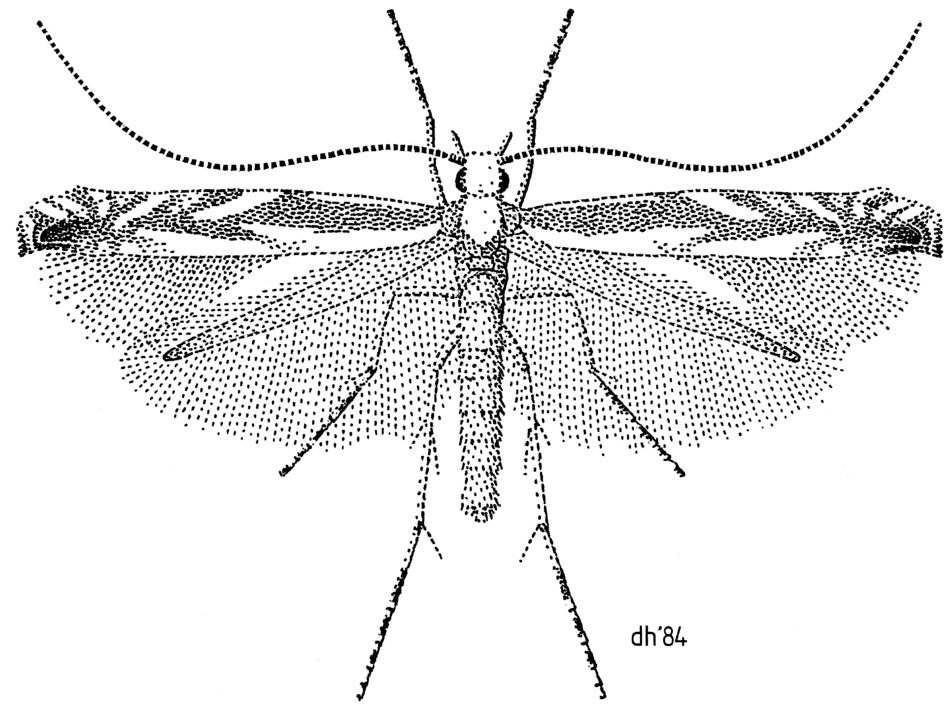
\includegraphics[width=0.5\textwidth]{amphiesmenoptera/gracillHab}
  \caption{Gracillariidae dorsal habitus. Illustration (CC BY 4.0) by Desmond Helmore, Manaaki Whenua - Landcare Research.}
  \label{fig:gracill2}
\end{figure}

\subsubsection{Gelechiidae (twirler moths, leaf tiers)}\index{Gelechiidae}
\noindent{}\textit{Diagnostic characters:} Small (wingspan 7--25 mm); maxillary palps short, 4-segmented, located close to base of proboscis; labial palps long, upcurved, 3rd segment elongate and tapering (figure \ref{fig:gelechiid1}); proboscis scaly; apical-posterior margin of hind wing concave (figure \ref{fig:gelechiid1}).\vspace{3mm}

\noindent{}\textit{Natural history:} Diversely phytophagous family, whose \textgreater4,500 described species mostly are generally found feeding internally on plants (\textit{e.g.}, in leaf mines and galls). This lineage includes many pest species, as well as moths that are important biocontrol agents against weeds. 

\begin{figure}[ht!]
  \centering
    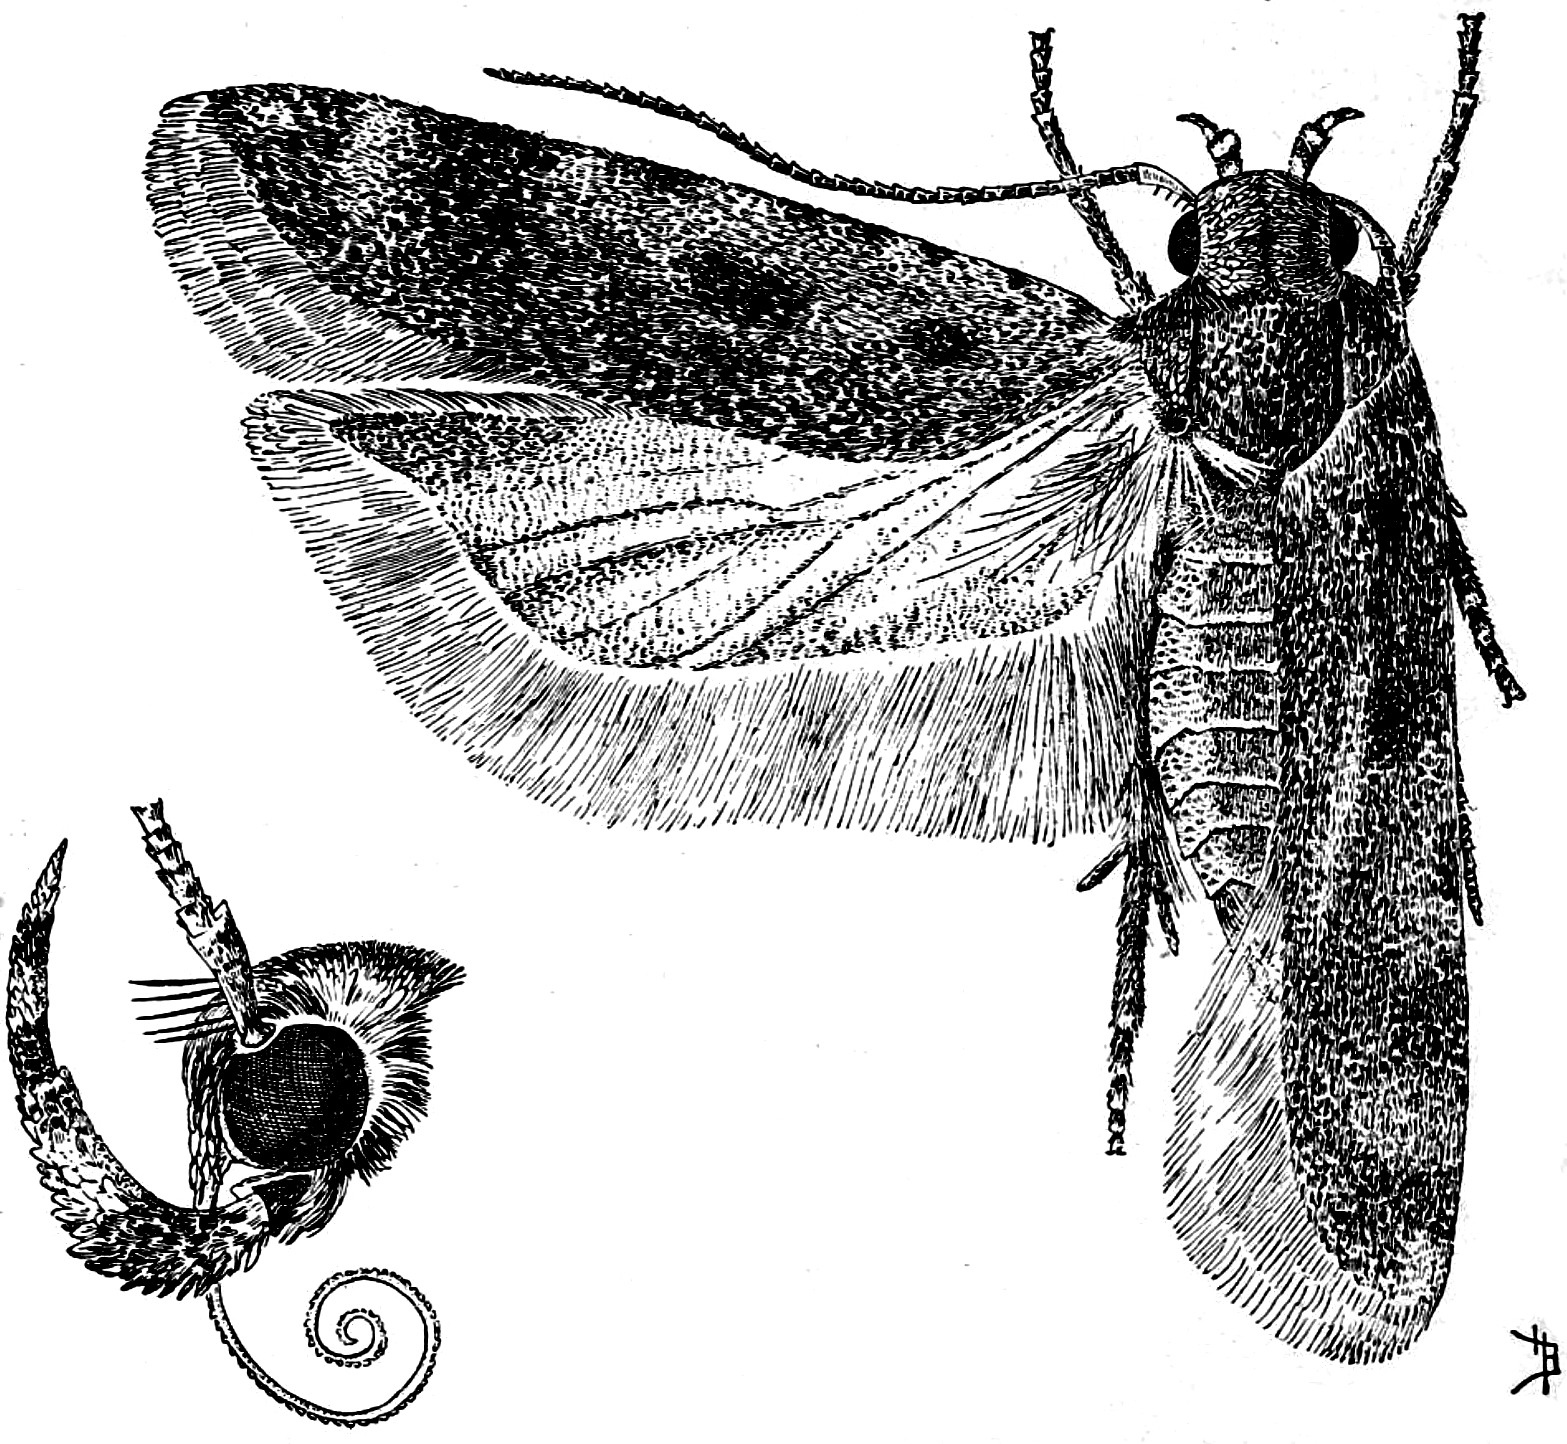
\includegraphics[width=0.5\textwidth]{amphiesmenoptera/gelechiidHabitus}
  \caption{Gelechiidae habitus and head \citep[modified from][Fig. 4]{bhlitem190298gelechiid}}
  \label{fig:gelechiid1}
\end{figure}

\subsubsection{Tineidae (clothes moths and relatives)}\index{Tineidae}
\noindent{}\textit{Diagnostic characters:} Small to medium-sized (wingspan 7--36 mm), usually gray or brown; head vestiture bushy, mostly comprised of erect scales (figure \ref{fig:tineid2}); antennae with a whorl of erect scales on each segment; maxillary palps usually present, folded; labial palps with sparse, elongate spines, usually very obvious; wing venation not so reduced as in above families (figure \ref{fig:tineid1}).\vspace{3mm}

\noindent{}\textit{Natural history:} Unlike most lepidopterans, species in this lineage mostly do \textit{not} feed on plants as larvae. Most species consume lichens, fungi, keratin (including feathers, mammal hair and horns), and detritus. About 3,000 species have been described worldwide.

\begin{figure}[ht!]
    \centering
    \begin{subfigure}[ht!]{0.45\textwidth}
        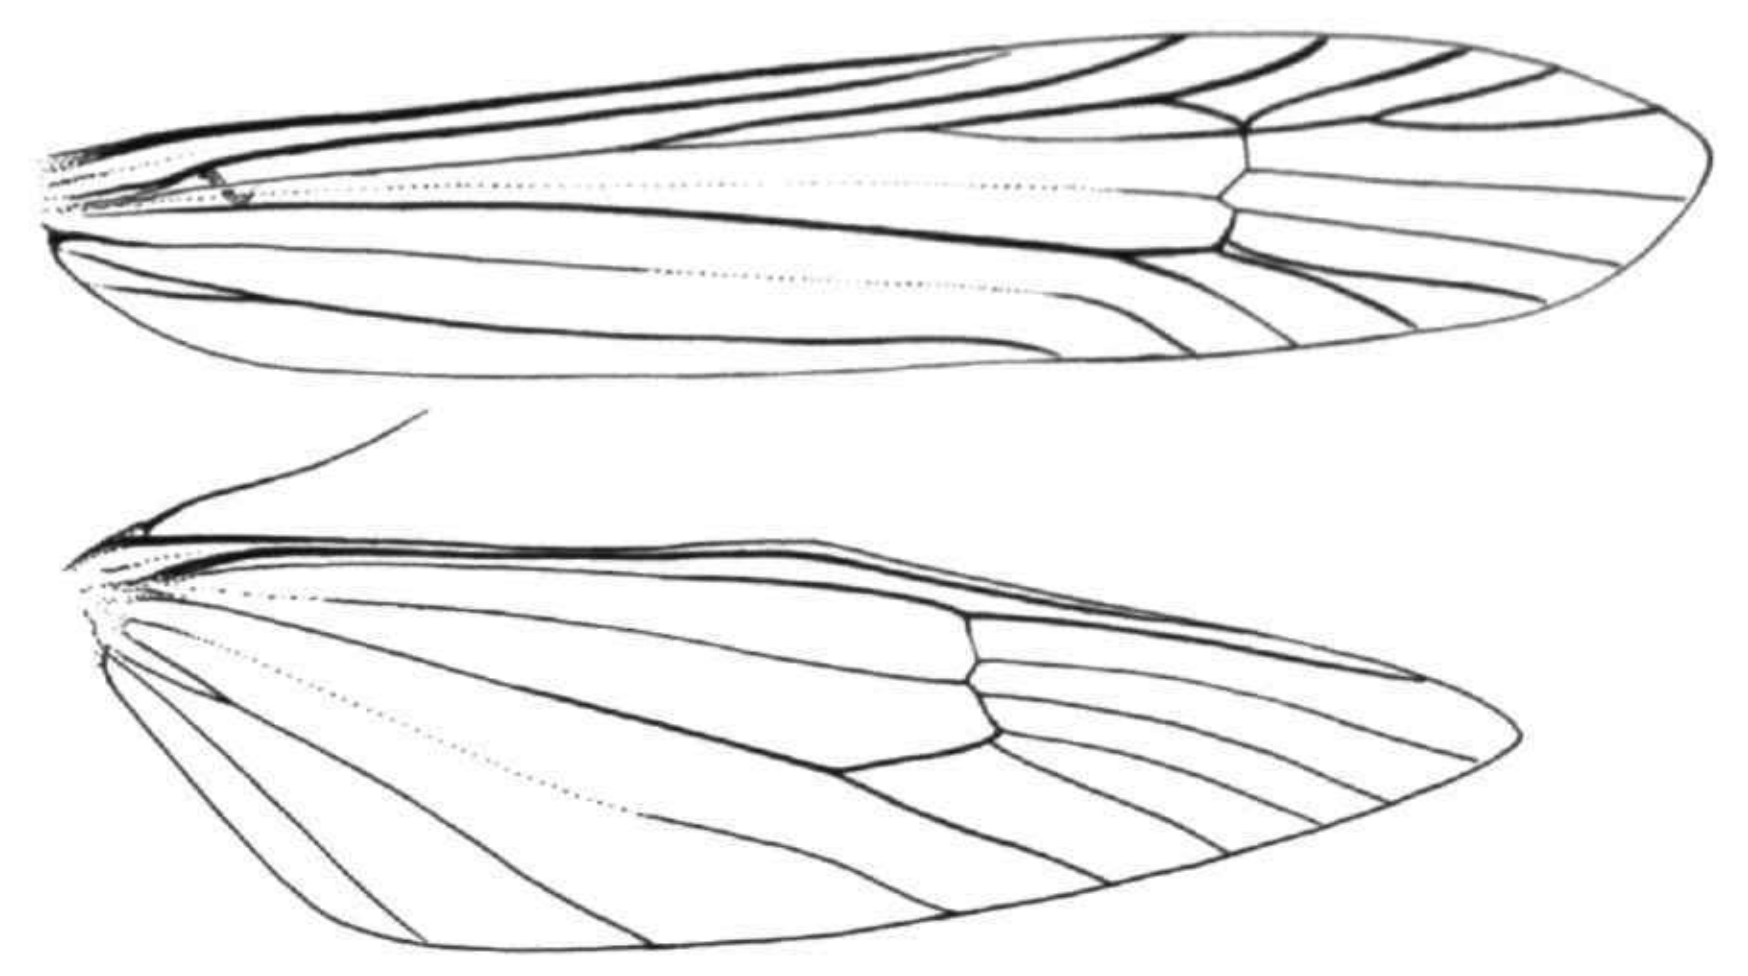
\includegraphics[width=\textwidth]{amphiesmenoptera/TineidWings}
        \caption{}
        \label{fig:tineid1}
    \end{subfigure}
    \hfill
    \begin{subfigure}[ht!]{0.50\textwidth}
        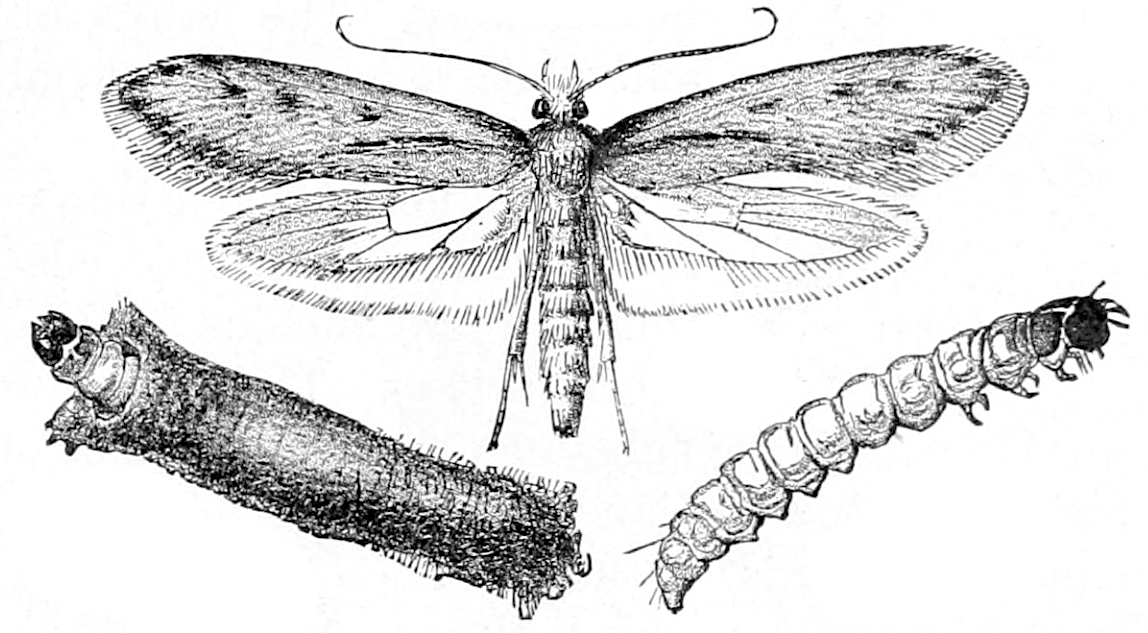
\includegraphics[width=\textwidth]{amphiesmenoptera/tineidHab}
        \caption{}
        \label{fig:tineid2}
    \end{subfigure}
    \caption{Tineidae. \textbf{(a)} Wings \citep[][Fig. 6]{DavisTineid1998}; \textbf{(b)} habitus \cite[][Fig. 17]{bhlitem20176riley}}\label{fig:tineids}
\end{figure}

\subsubsection{Psychidae (bagworm moths)}\index{Psychidae}
\noindent{}\textit{Diagnostic characters:} Small to medium-sized moths (wingspan 12--36 mm); body usual black in North American species \ref{fig:psychid3}; wings often absent or reduced in females, which often remain in the silken bag (figure \ref{fig:psychid2}); male wings often (but not always!) mostly clear; setae hair-like, rather than scale-like.\vspace{3mm}

\noindent{}\textit{Natural history:} Larvae typically form bags constructed of silk and plant material. Females usually have only vestigial wings and often remain inside these cases after pupation. Males are winged and only rarely colorful. Almost 1,350 species have been described.

\begin{figure}[ht!]
    \centering
    \begin{subfigure}[ht!]{0.35\textwidth}
        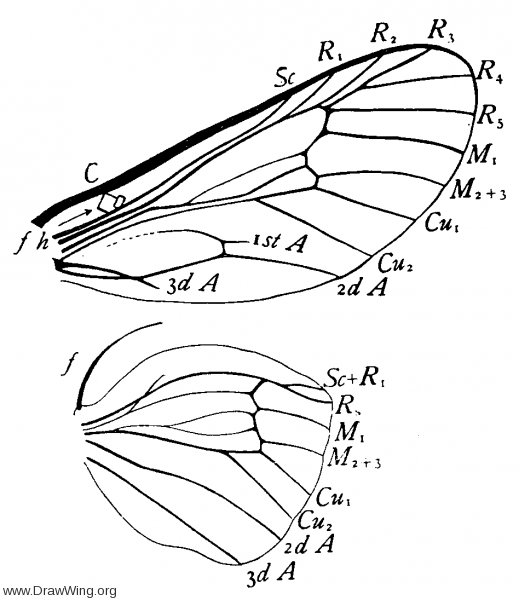
\includegraphics[width=\textwidth]{amphiesmenoptera/PsychidWings}
        \caption{}
        \label{fig:psychid1}
    \end{subfigure}
    \hfill 
    \begin{subfigure}[ht!]{0.13\textwidth}
        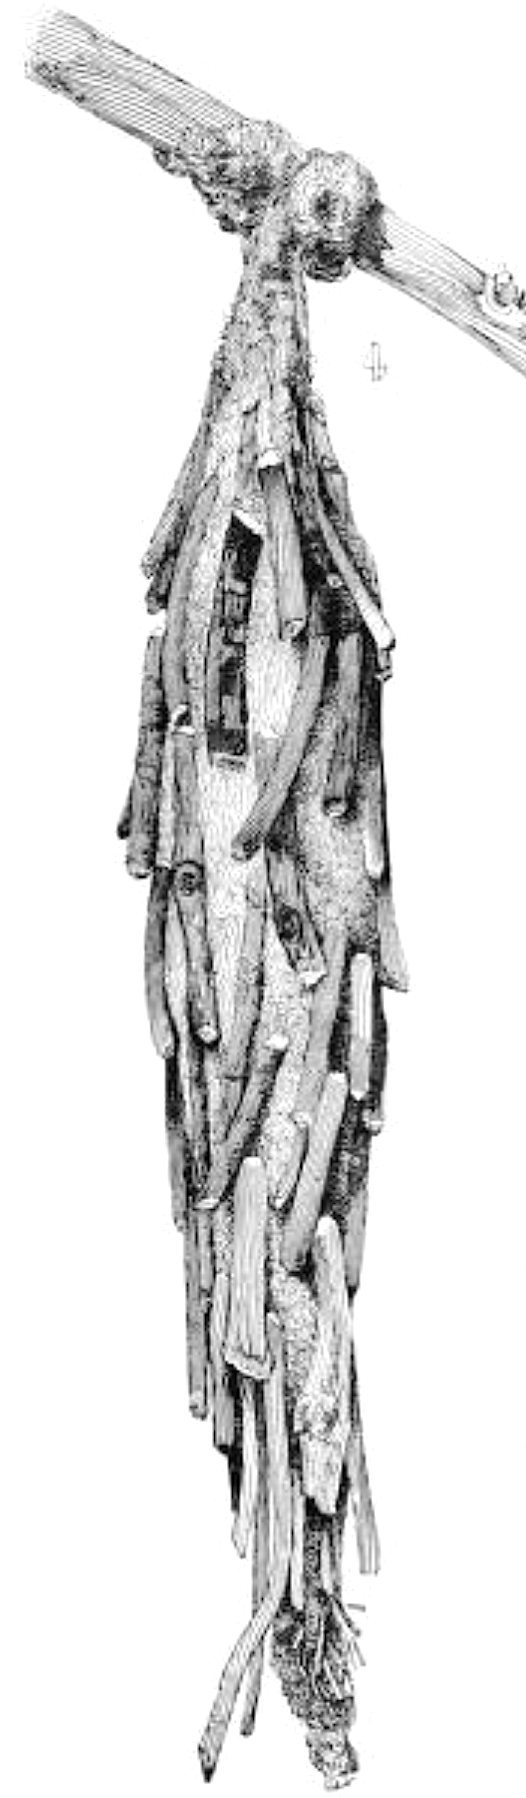
\includegraphics[width=\textwidth]{amphiesmenoptera/psychidBag}
        \caption{}
        \label{fig:psychid2}
    \end{subfigure}
    \hfill 
    \begin{subfigure}[ht!]{0.42\textwidth}
        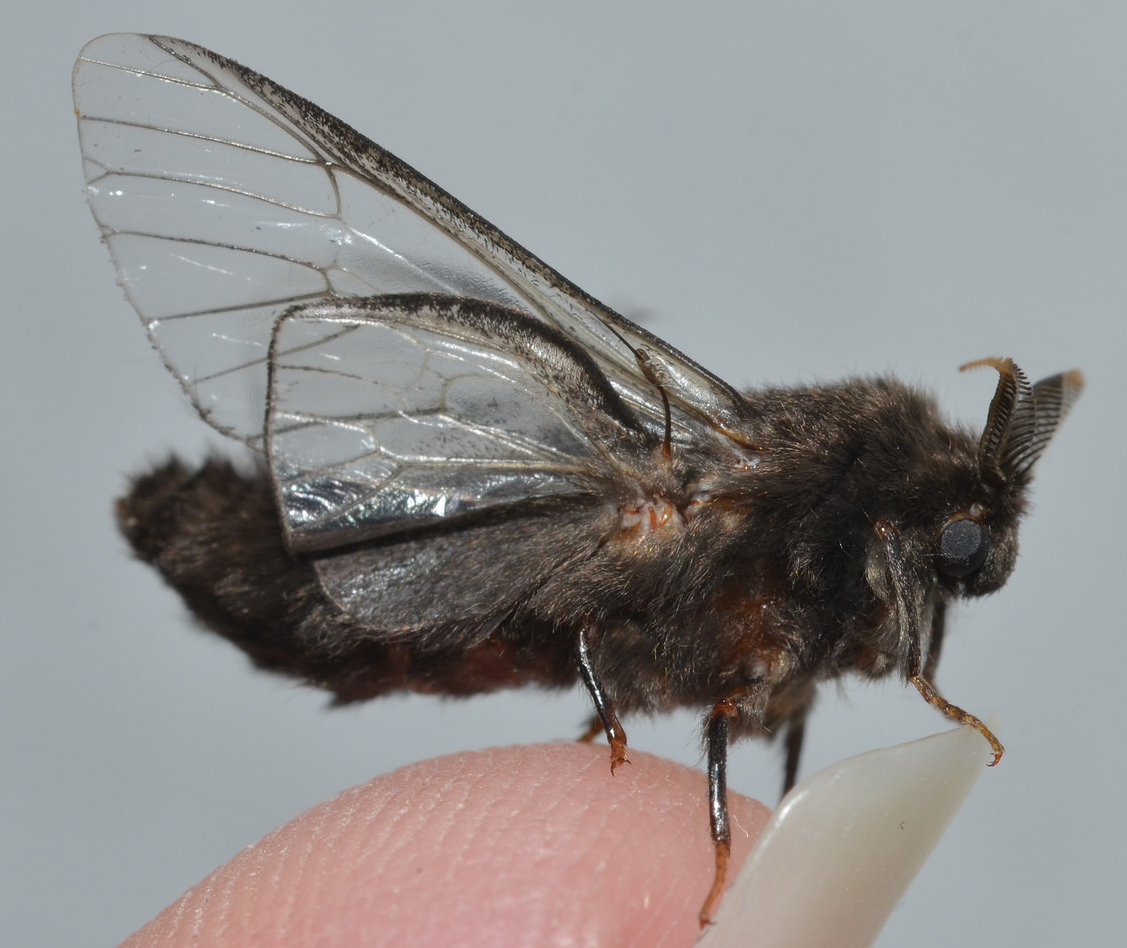
\includegraphics[width=\textwidth]{amphiesmenoptera/PsychidHabitus}
        \caption{}
        \label{fig:psychid3}
    \end{subfigure}
    \caption{Psychidae. \textbf{(a)} Wings \citep[Fig. 46]{comstock1918wings}; \textbf{(b)} mature case \citep[][plate XXV, Fig. 4]{bhlitem82061AustrInsect}; \textbf{(c)} habitus \citep[][Fig. 374A]{escherich1914forstinsekten}}\label{fig:psychids}
\end{figure}

\subsubsection{Sesiidae (clearwing moths)}\index{Sesiidae}
\noindent{}\textit{Diagnostic characters:} Small to medium-sized (wingspan 15--50 mm); transparent, scaleless ``windows'' usually present on wings; often wasp-like in shape and color (figure \ref{fig:sesiid2}); antennae widen apically, but narrow at the apex and are often somewhat hooked.\vspace{3mm}

\noindent{}\textit{Natural history:} These moths are usually diurnal; can you guess why? Most species are wood or stem borers, and the taxon includes many pestiferous species. More than 1,300 species have been described.

\begin{figure}[ht!]
    \centering
    \begin{subfigure}[ht!]{0.4\textwidth}
        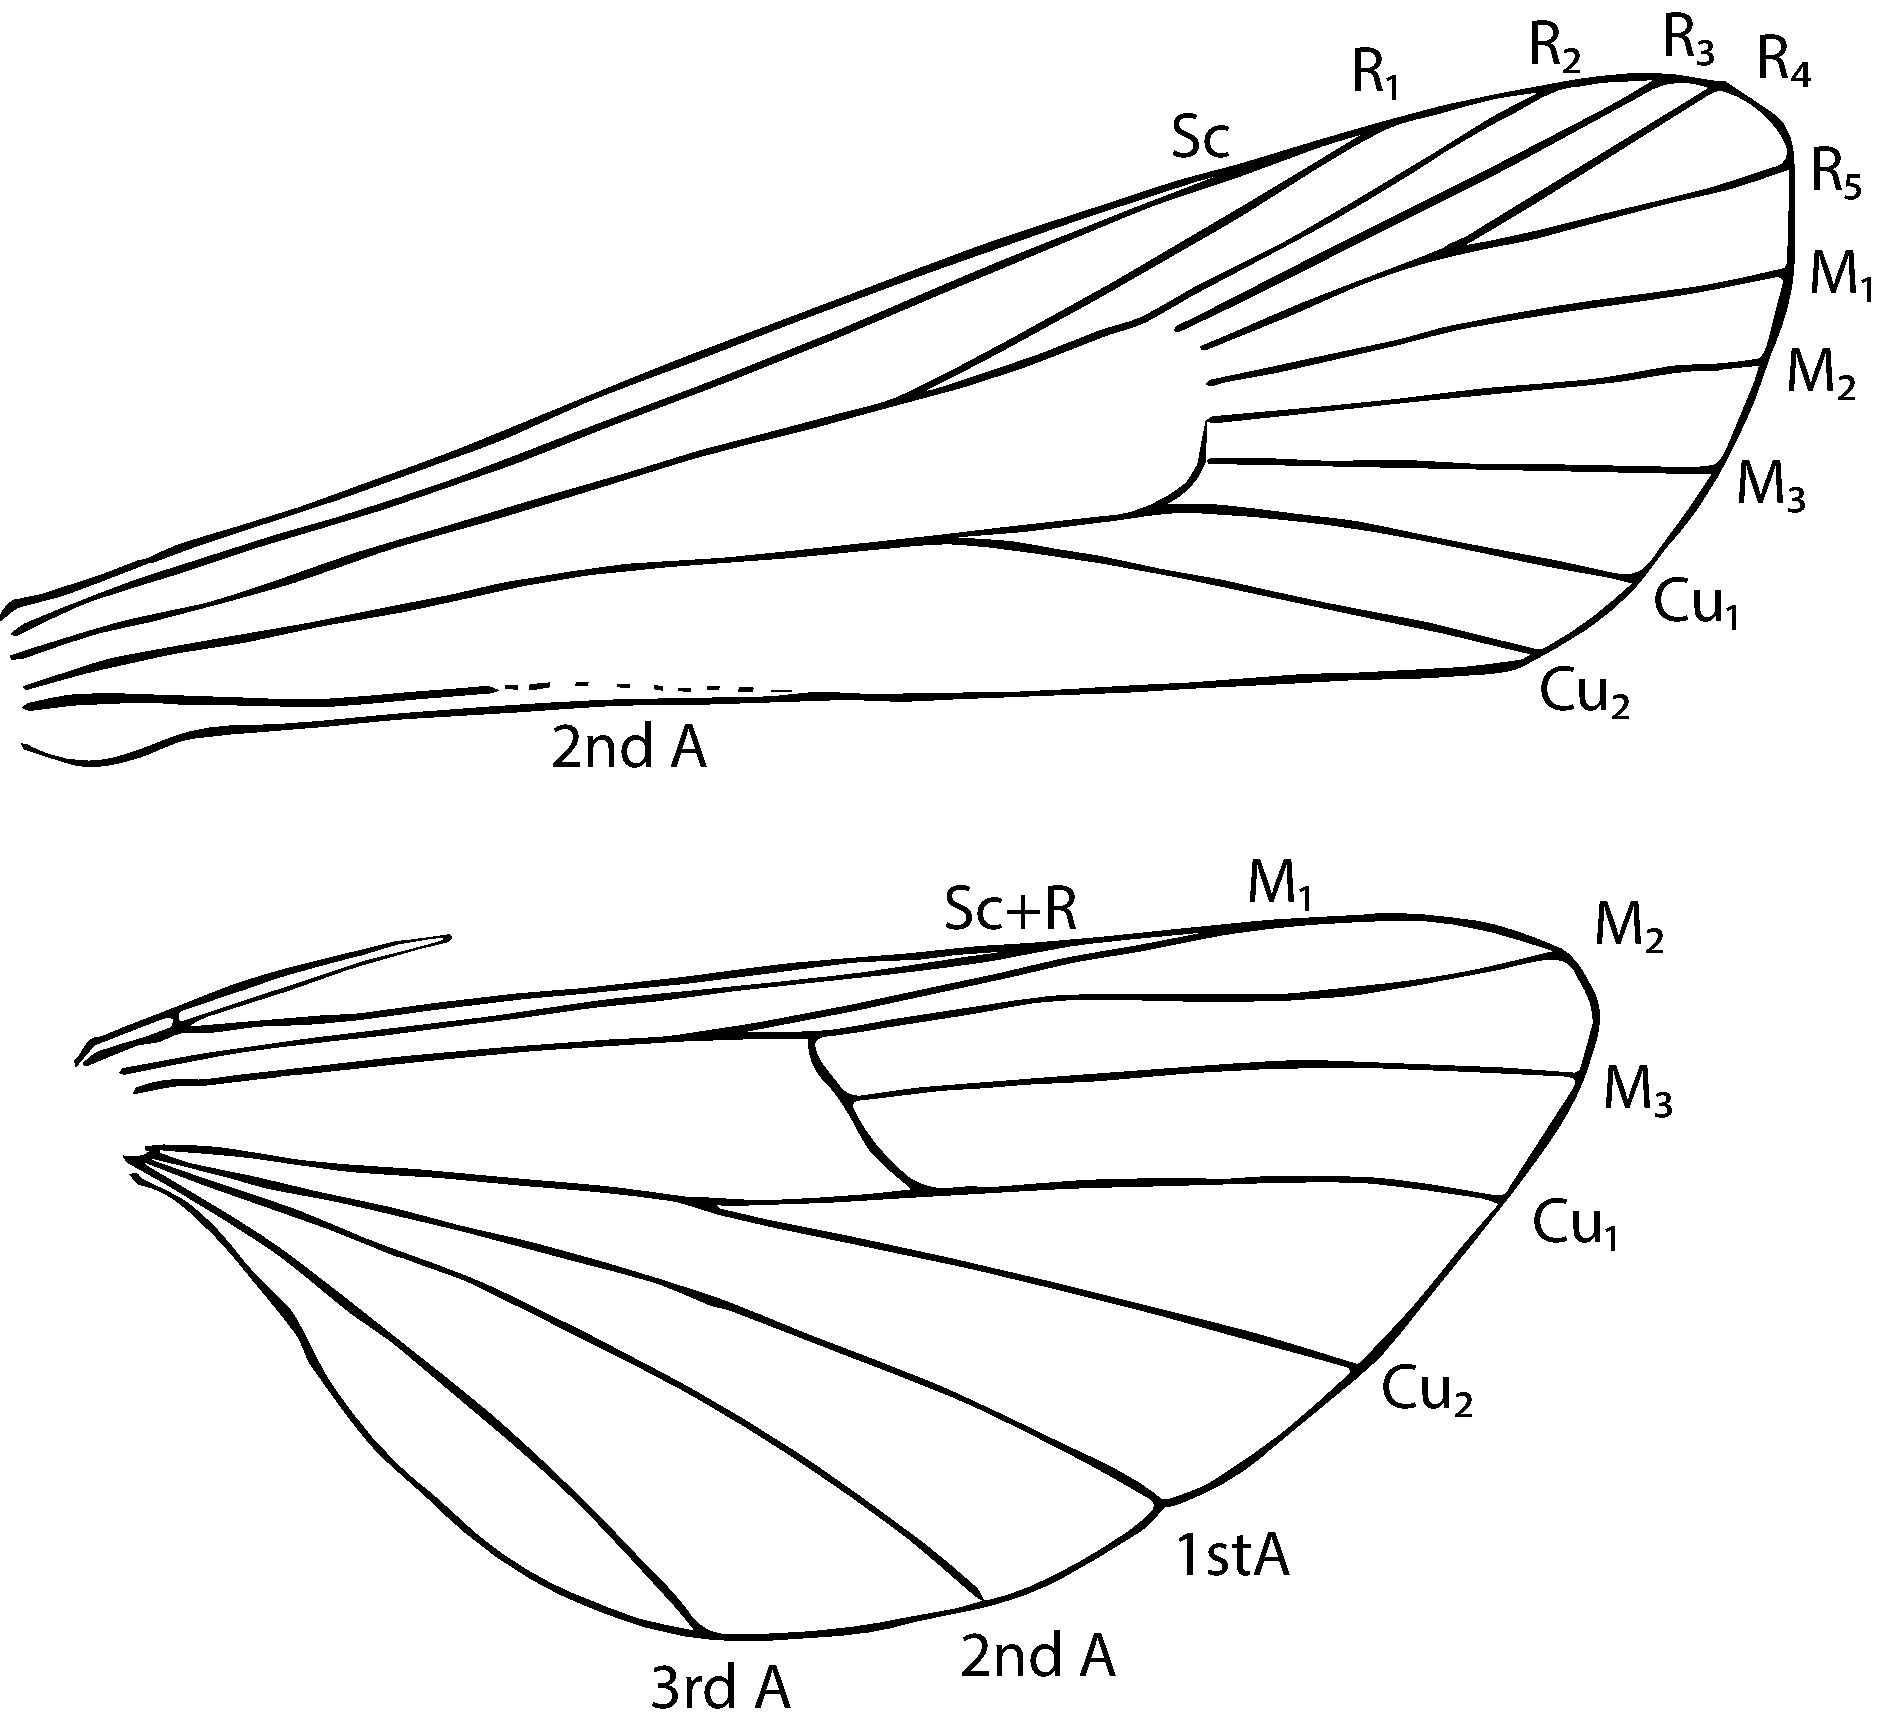
\includegraphics[width=\textwidth]{amphiesmenoptera/SesiidWings}
        \caption{}
        \label{fig:sesiid1}
    \end{subfigure}
    \hfill 
    \begin{subfigure}[ht!]{0.52\textwidth}
        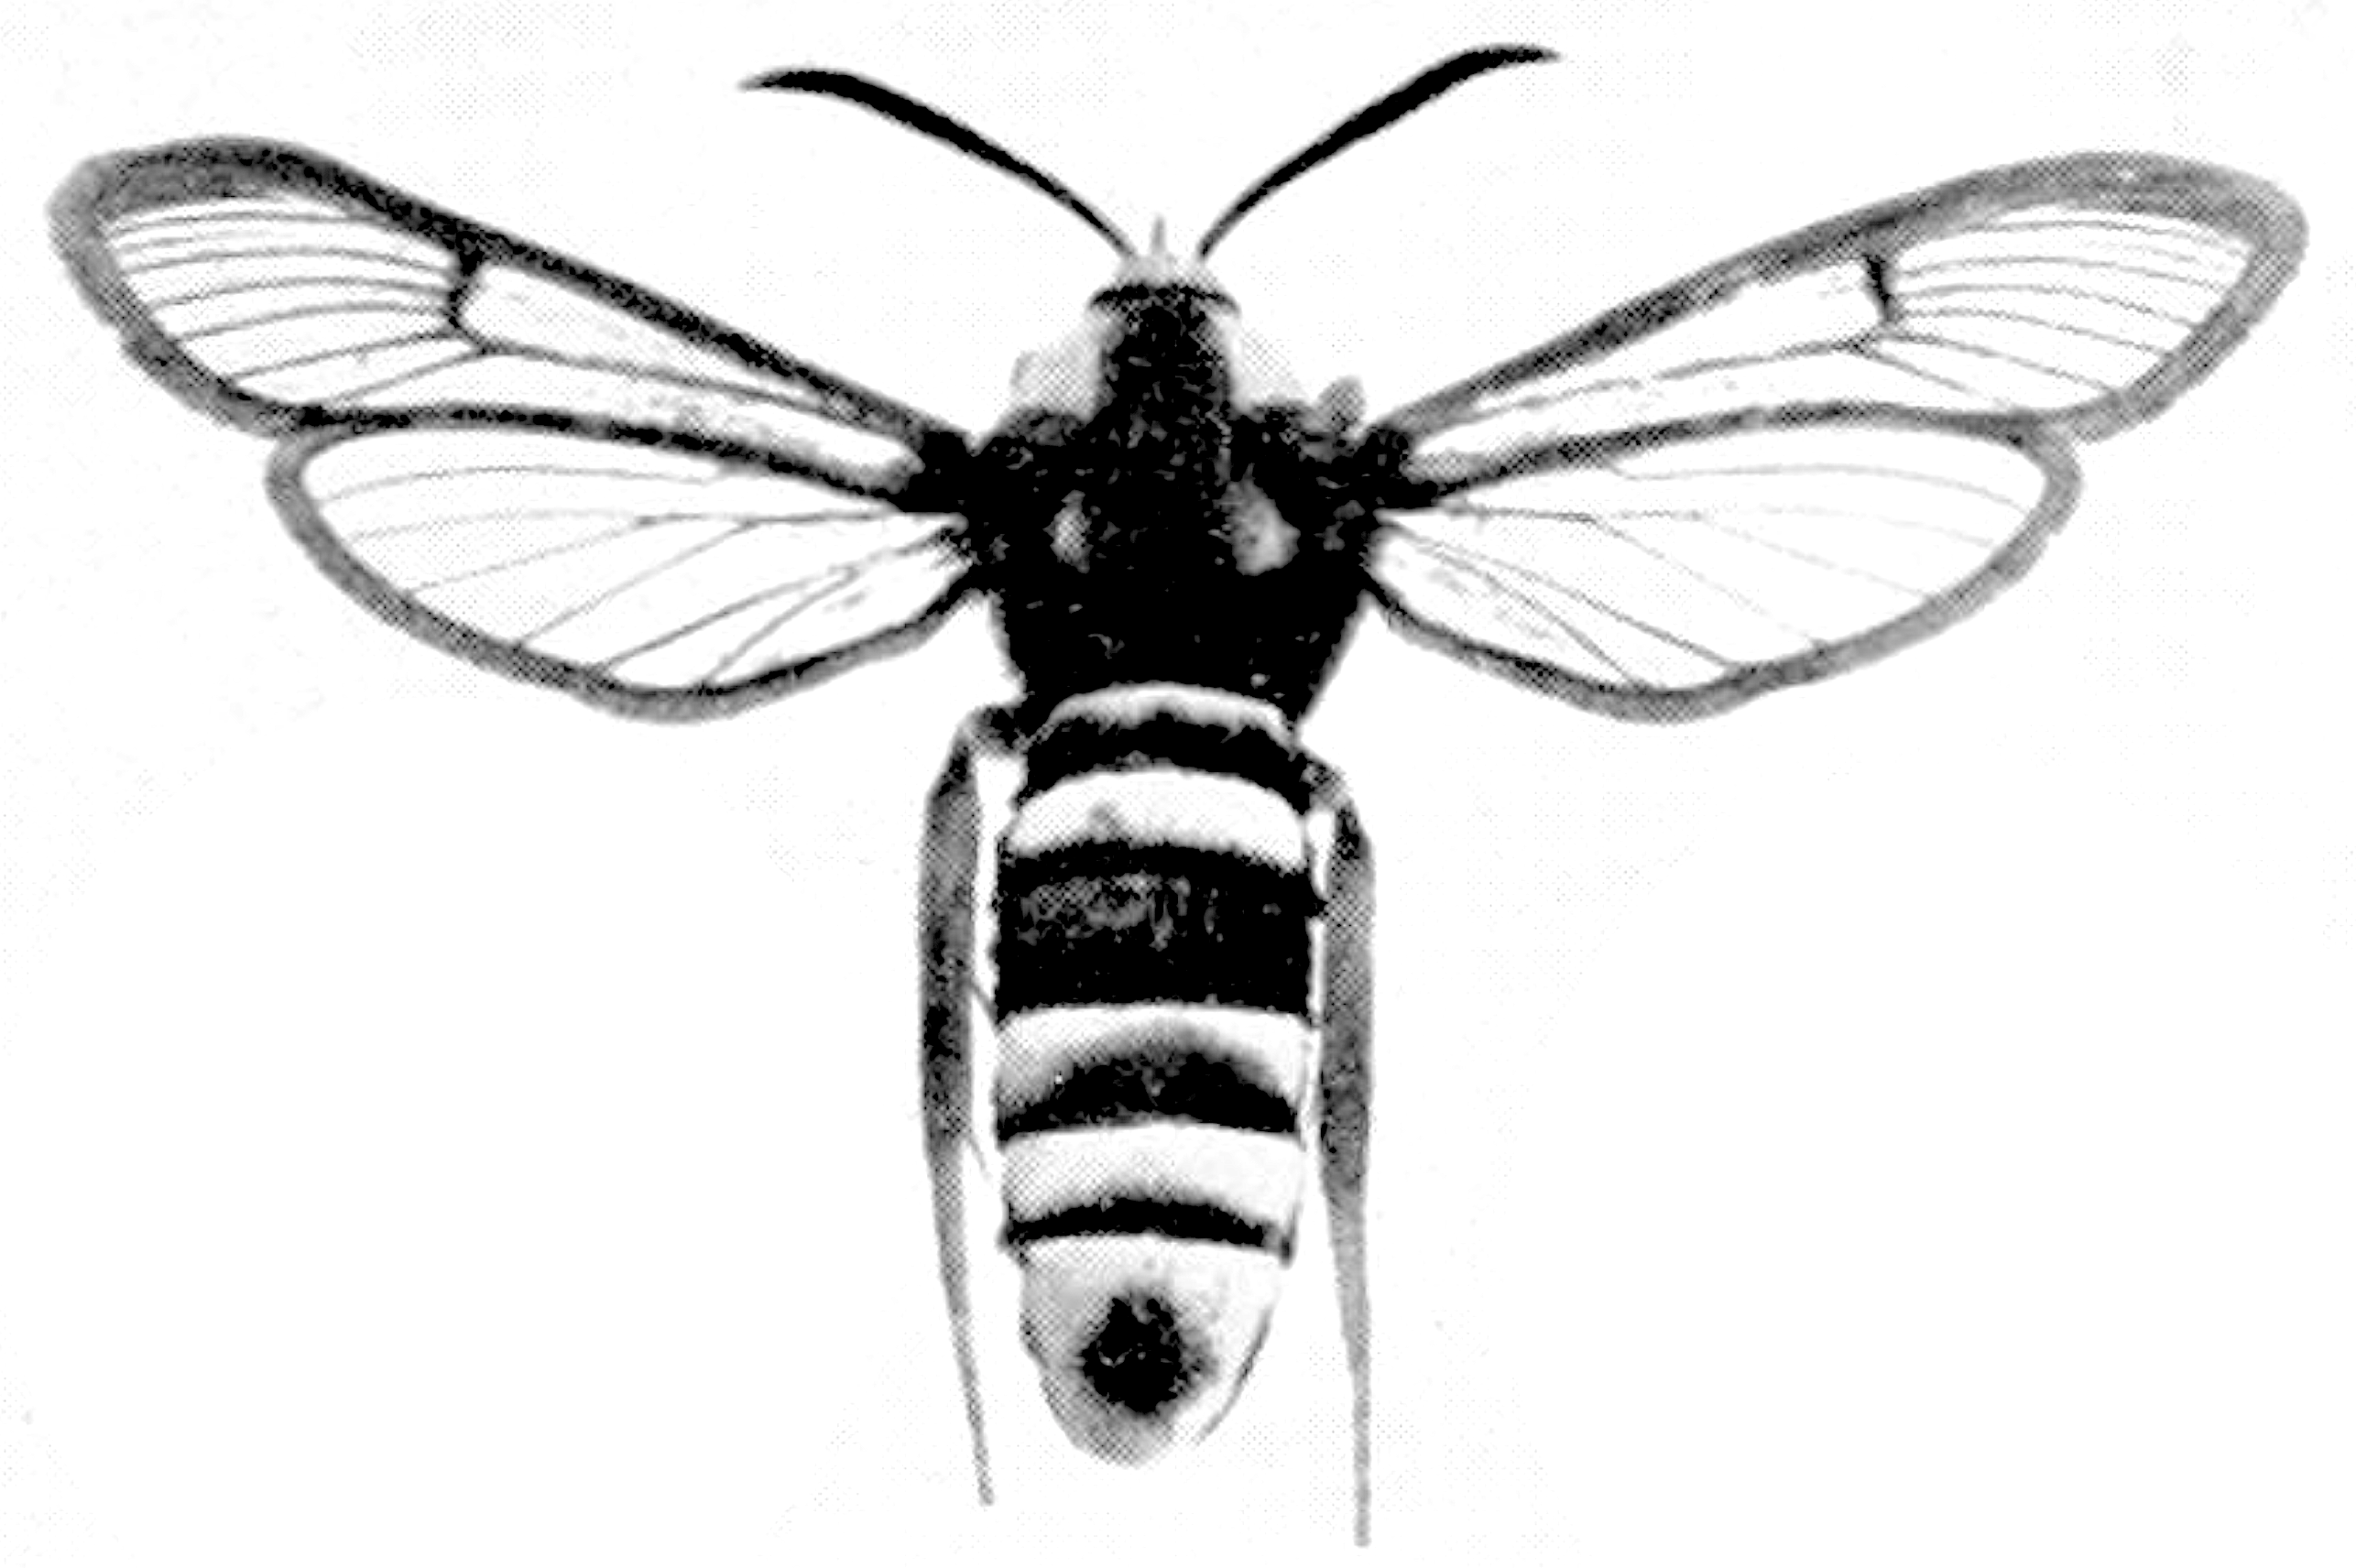
\includegraphics[width=\textwidth]{amphiesmenoptera/sesiidHab}
        \caption{}
        \label{fig:sesiid2}
    \end{subfigure}
    \caption{Sesiidae. (a) Wings \citep[][Fig. 8]{bhl118765}; (b) habitus \citep[][Fig. 351A]{escherich1914forstinsekten}}\label{fig:sesiids}
\end{figure}

\subsubsection{Cossidae (carpenterworm moths)}\index{Cossidae}
\noindent{}\textit{Diagnostic characters:} Relatively large (wingspan 40--100 mm), mottled gray and brown, heavy-bodied moths; male antennae bipectinate, females filliform; species in the U.S. usually black and gray, dull or with some orange; head is relatively small compared to the rest of the body (as opposed to Sphingidae) (figure \ref{fig:cossid2}).\vspace{3mm}

\noindent{}\textit{Natural history:} There are almost 700 species worldwide, but only a handful occur in North America. Most species are borers, and a few are pests. About 700 species have been described worldwide.\vspace{3mm}

\begin{figure}[ht!]
    \centering
    \begin{subfigure}[ht!]{0.35\textwidth}
        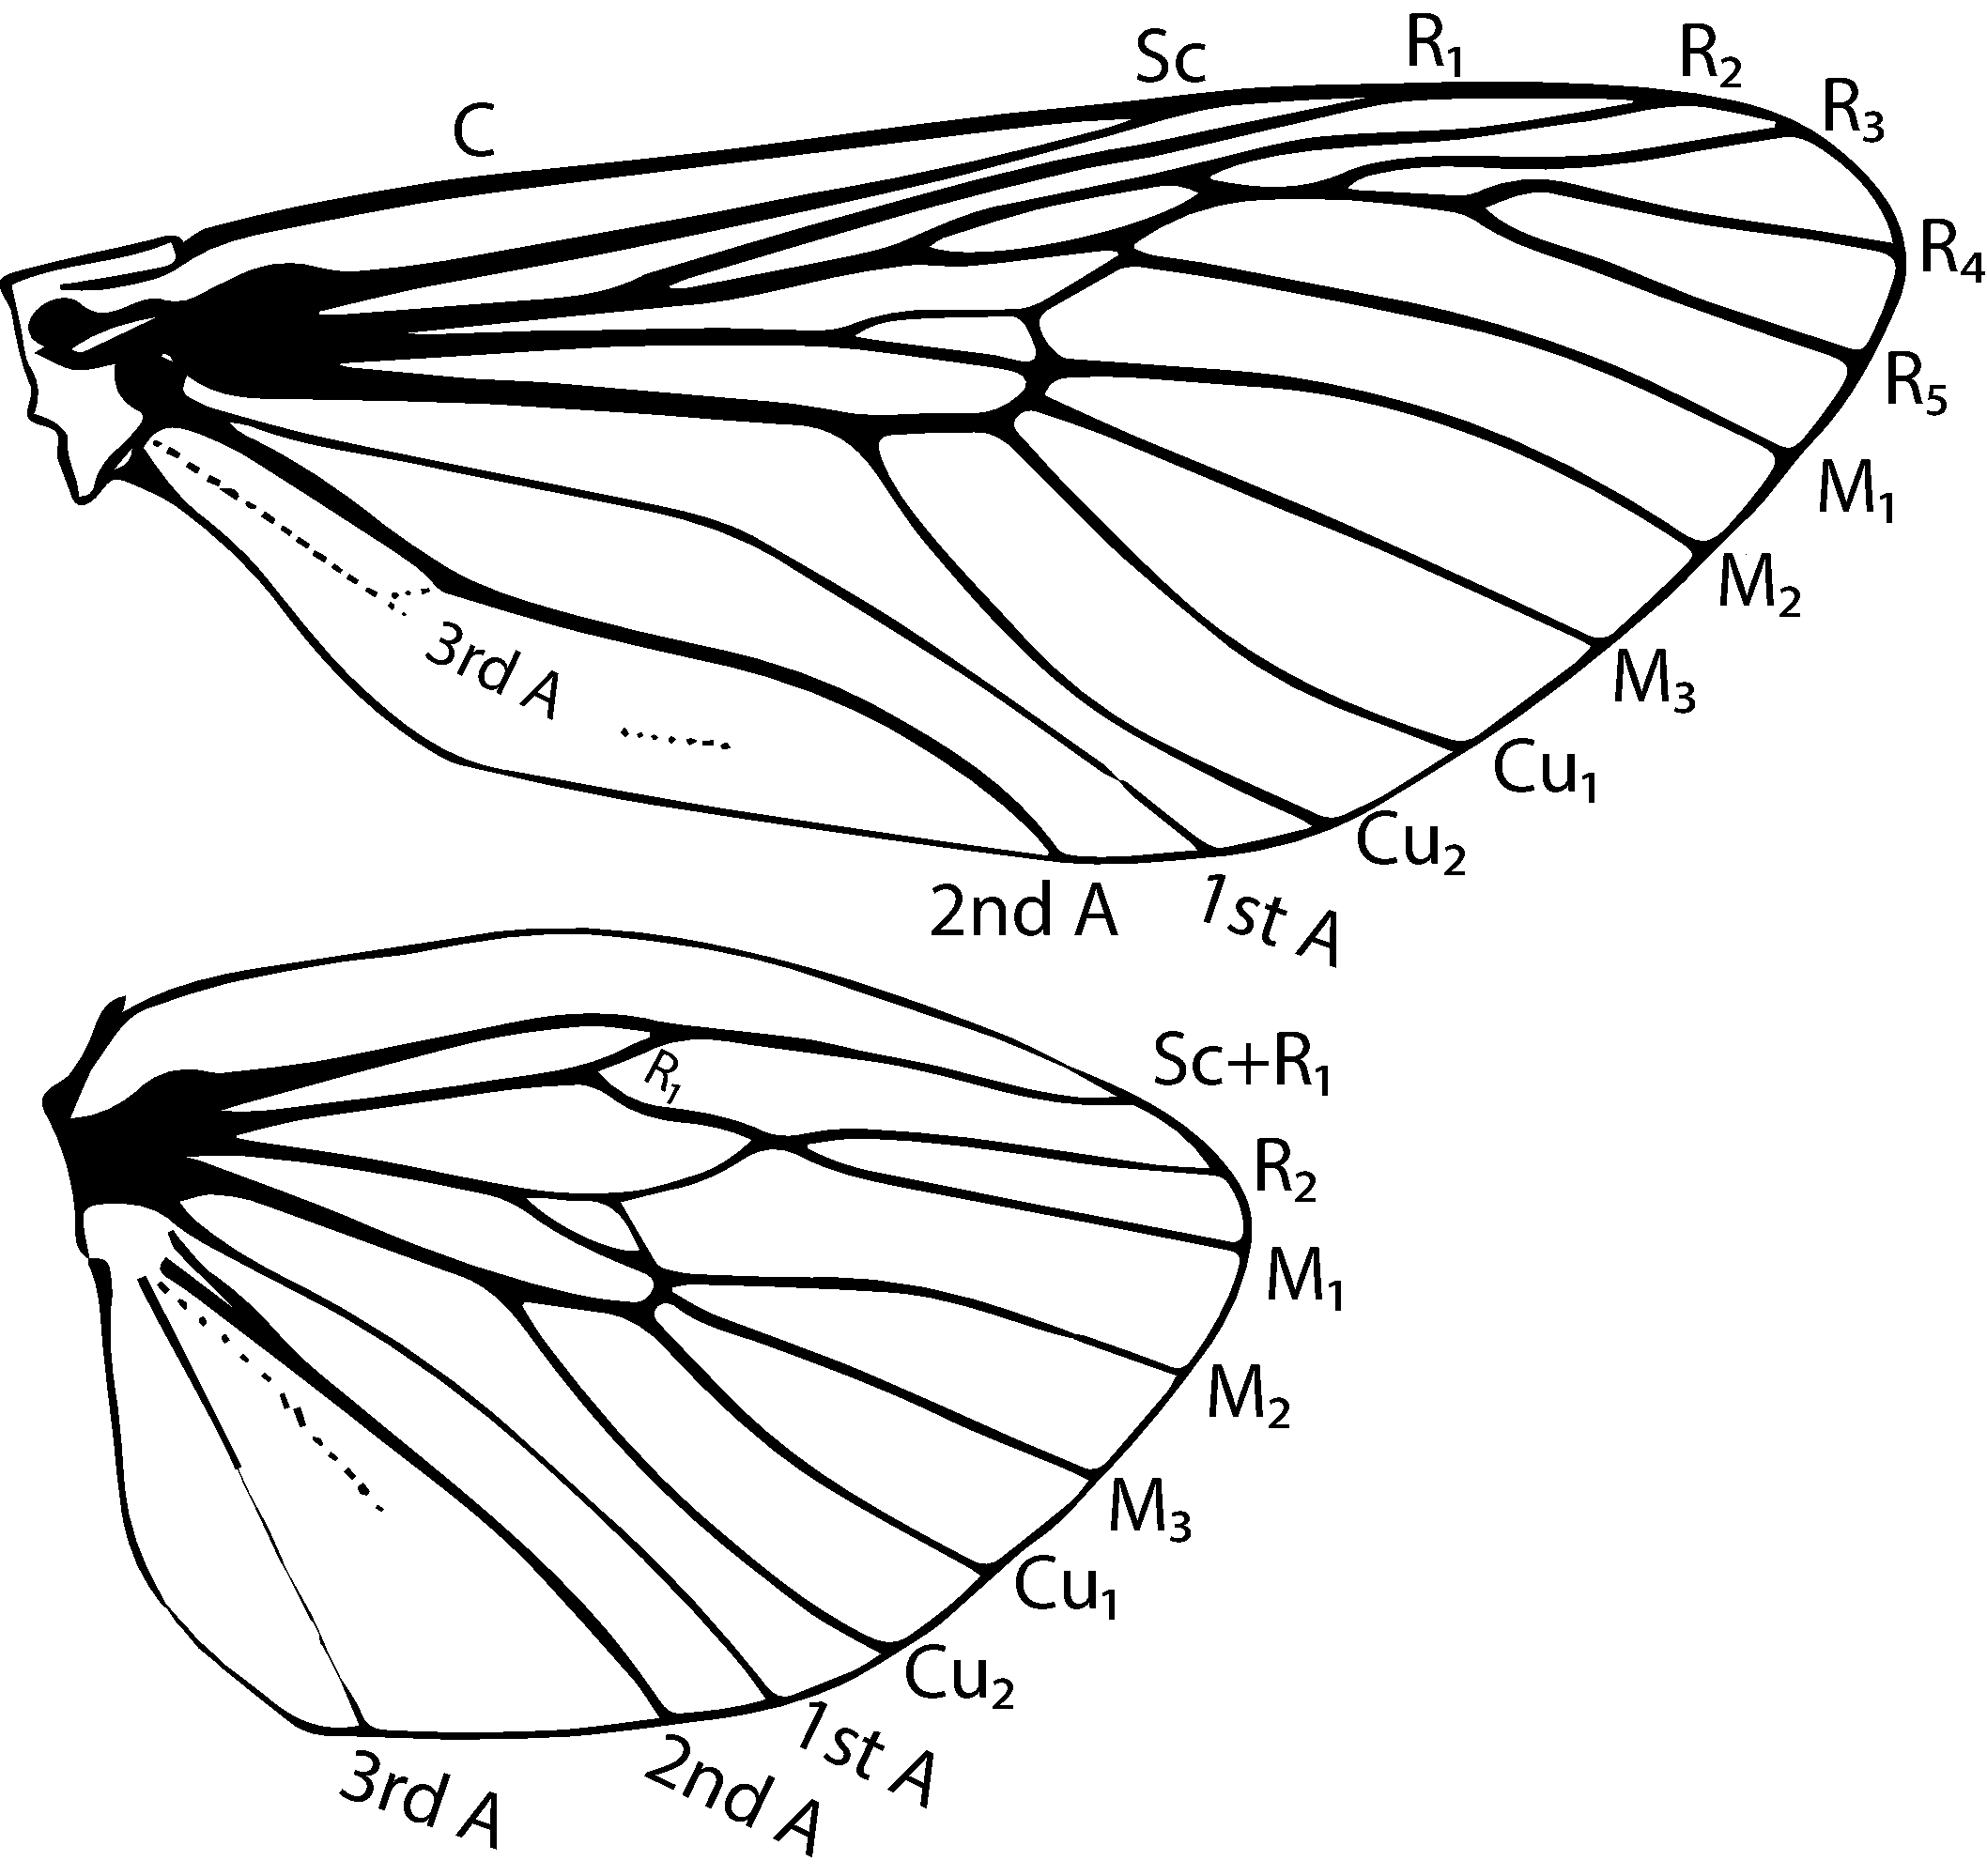
\includegraphics[width=\textwidth]{amphiesmenoptera/CossidWings}
        \caption{}
        \label{fig:cossid1}
    \end{subfigure}
    \hfill 
    \begin{subfigure}[ht!]{0.6\textwidth}
        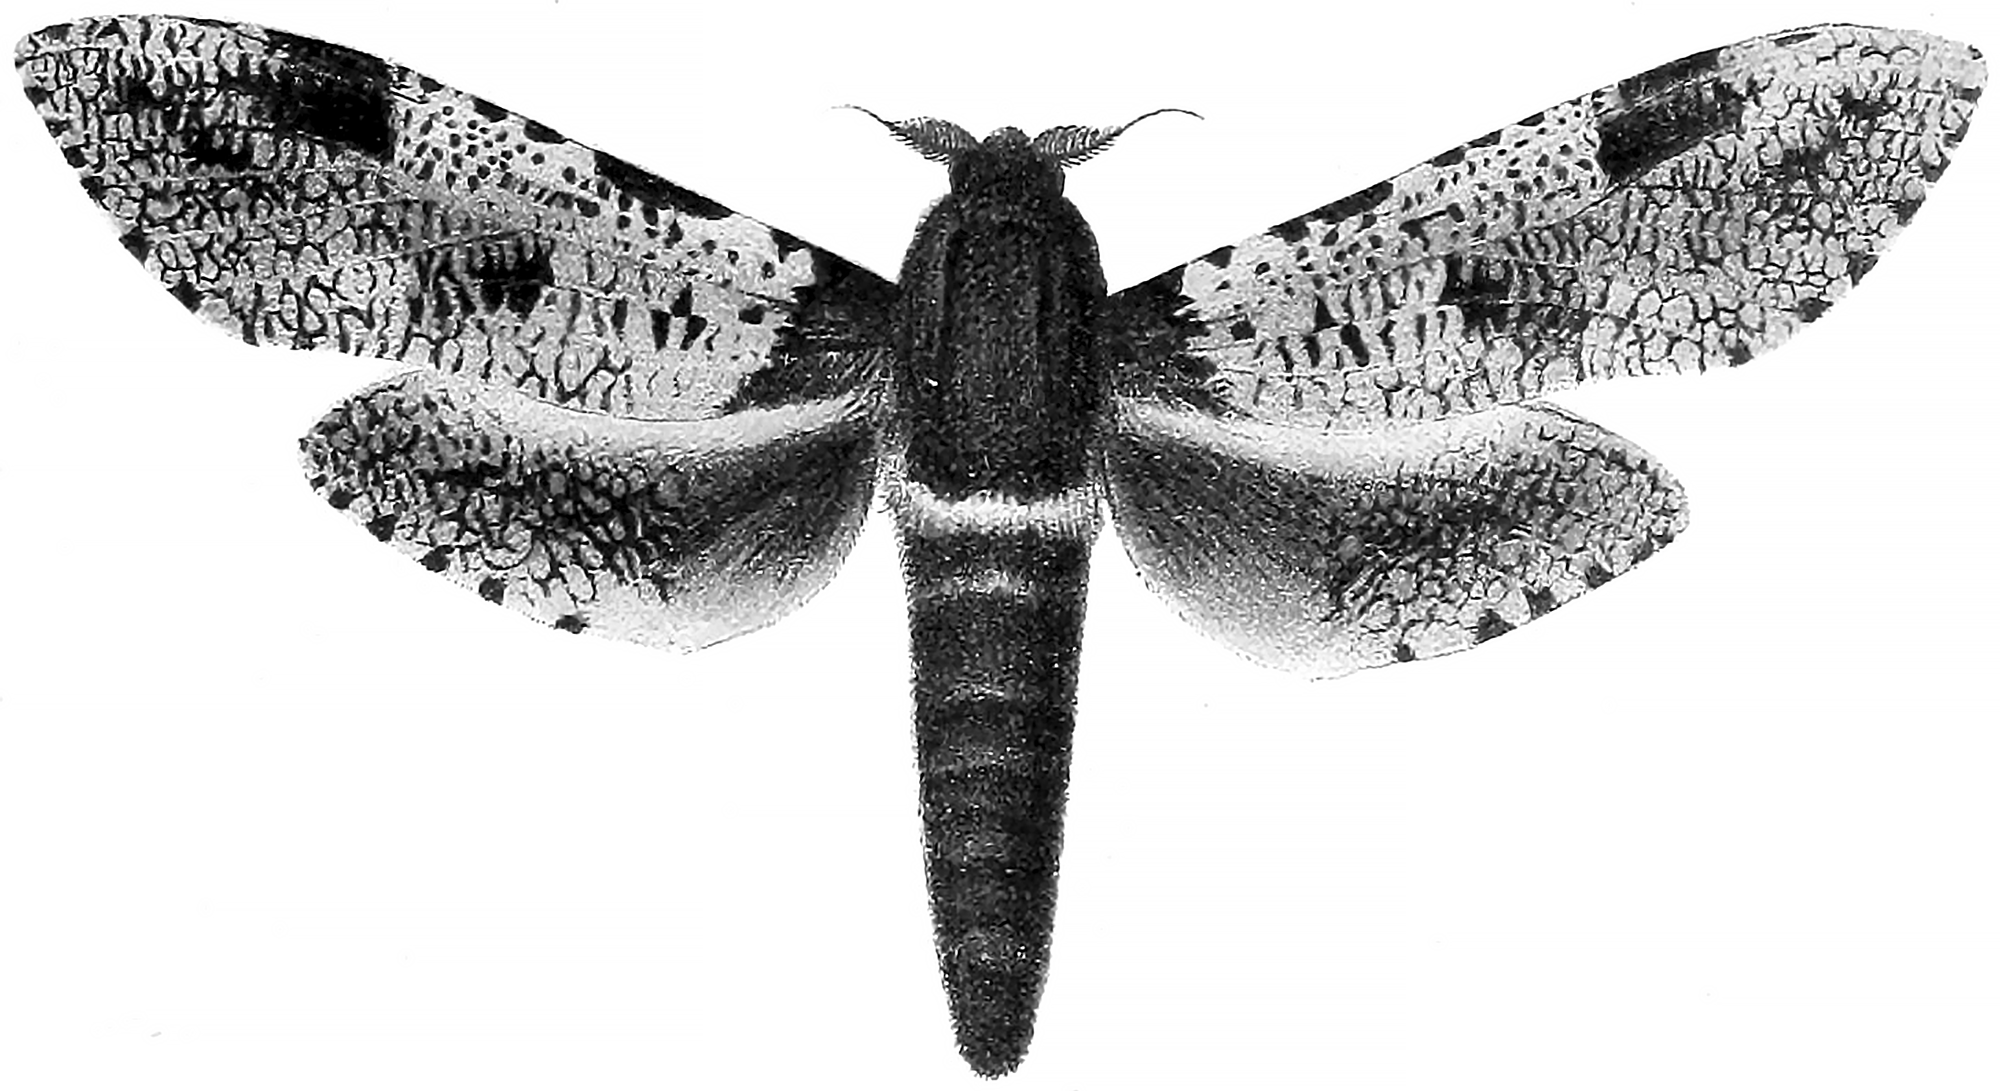
\includegraphics[width=\textwidth]{amphiesmenoptera/CossidaeHabitus}
        \caption{}
        \label{fig:cossid2}
    \end{subfigure}
    \caption{Cossidae. \textbf{(a)} Wings \citep[Fig. 343]{comstock1918wings}; \textbf{(b)} habitus \citep[modified from][plate 97, fig. b]{bhlitem38567}}\label{fig:cossids}
\end{figure}

\subsubsection{Tortricidae (leafroller and fruitworm moths)}\index{Tortricidae}
\noindent{}\textit{Diagnostic characters:} Small to medium-sized moths (wingspan 10--33 mm); labial palps usually project forward (figure \ref{fig:tortricid2}), maxillary palps small; portions of scales on head often flattened; apical margin of fore wings usually distinctive, broad (figure \ref{fig:tortricid1}); fore wings with complex color pattern relative to hind wings.\vspace{3mm}

\noindent{}\textit{Natural history:} Diverse lineage, with \textgreater10,000 species, including many important pests. Larvae are diversely phytophagous, being leaf rollers, leaf tiers, fruit borers, gallers, \textit{etc}. Well over 10,000 species have been described.

\begin{figure}[ht!]
    \centering
    \begin{subfigure}[ht!]{0.35\textwidth}
        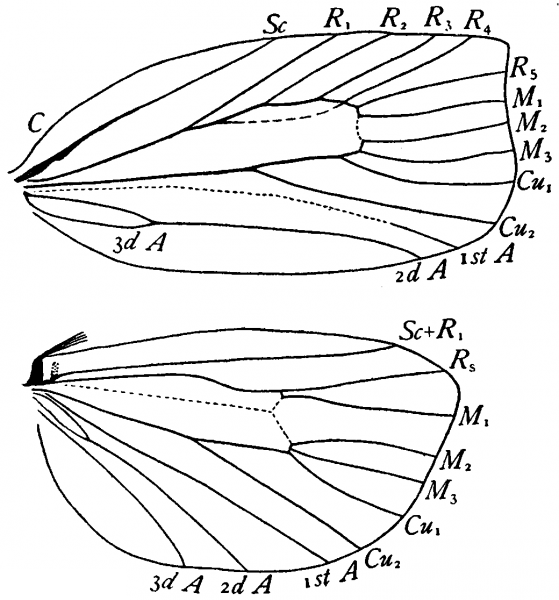
\includegraphics[width=\textwidth]{amphiesmenoptera/TortricidWings}
        \caption{}
        \label{fig:tortricid1}
    \end{subfigure}
    \qquad
    \begin{subfigure}[ht!]{0.55\textwidth}
        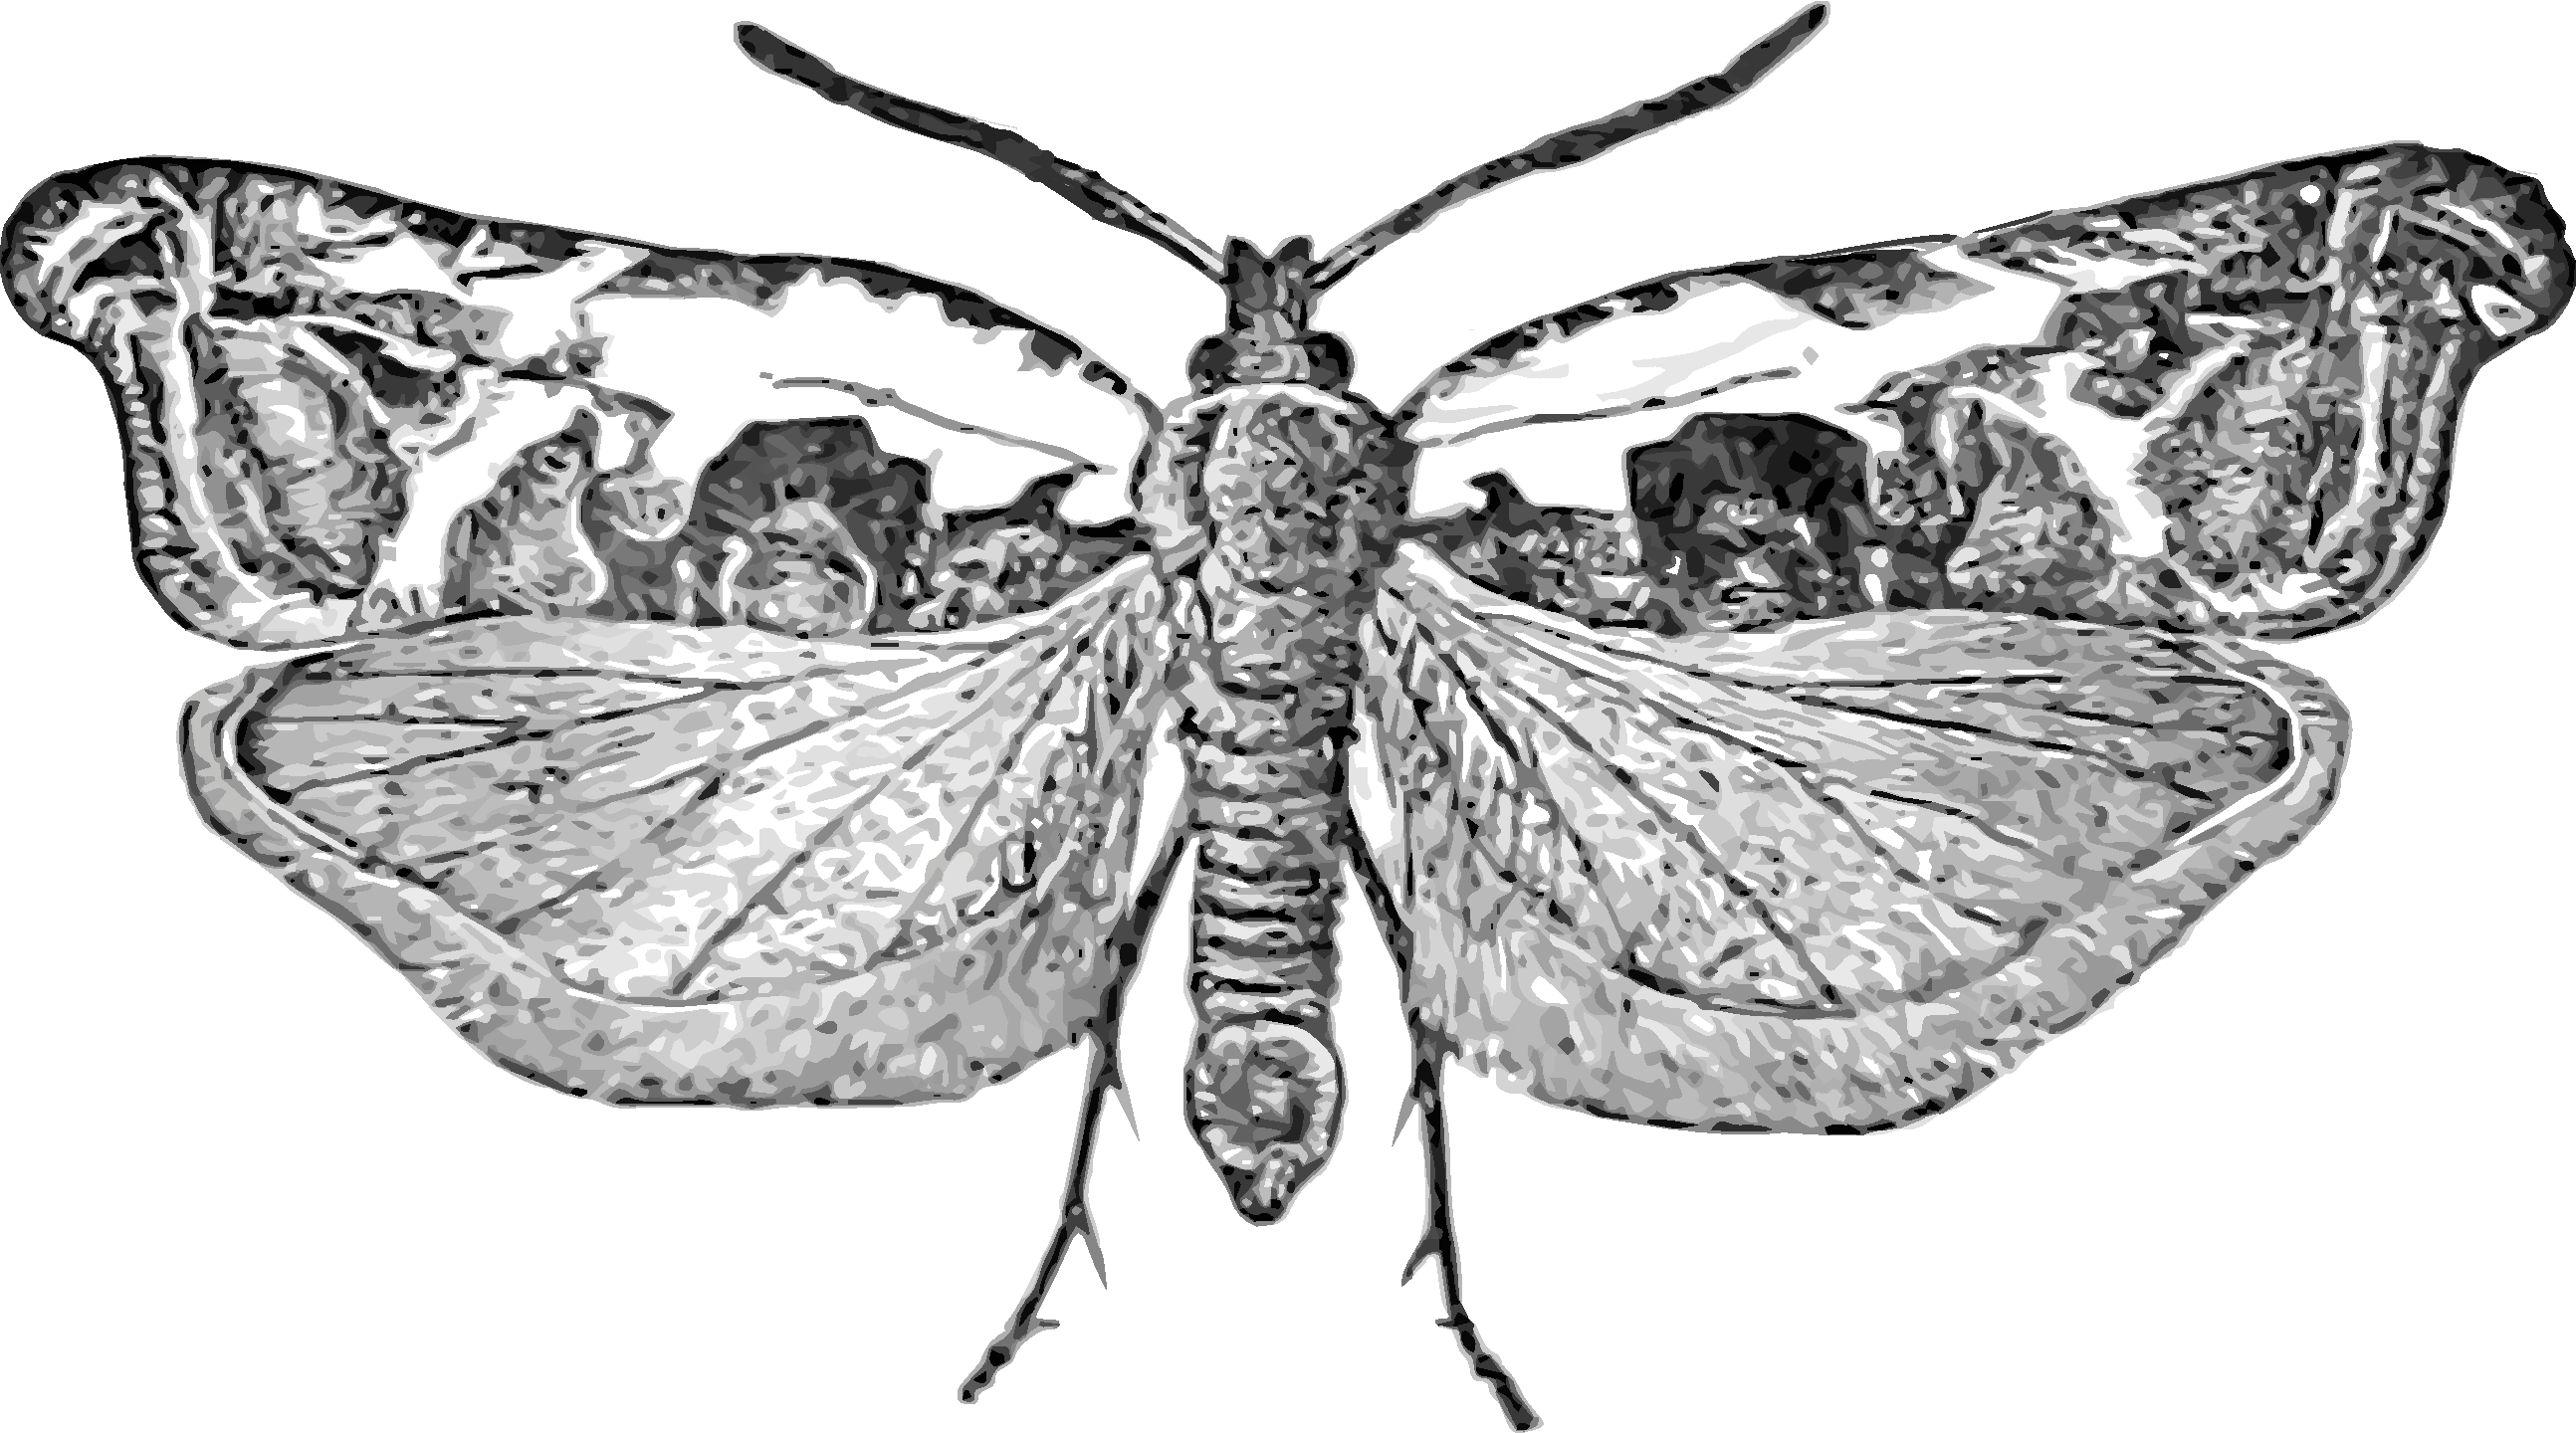
\includegraphics[width=\textwidth]{amphiesmenoptera/tortricidHab}
        \caption{}
        \label{fig:tortricid2}
    \end{subfigure}
    \caption{Tortricidae. \textbf{(a)} Wings \citep[Fig. 353]{comstock1918wings}; \textbf{(b)} habitus \citep[][Fig. 96]{saunders1883insects}}\label{fig:tortricids}
\end{figure}

\subsubsection{Limacodidae (slug caterpillar moths)}\index{Limacodidae}
\noindent{}\textit{Diagnostic characters:} Stout-bodied; usually brown and green or brown and silver (figure \ref{fig:limacodid2}); fore wing with 2 complete anal veins (figure \ref{fig:limacodid1}); Sc and R in hind wing separate at base, then briefly fused; hind wing with 3 anal veins.\vspace{3mm}

\noindent{}\textit{Natural history:} Larvae usually have reduced legs and prolegs and locomote with the assistance of silk. They are often defended by urticating setae. Cocoons are fashioned in a characteristic cup-shape. Adults often adopt bizarre postures when stationary on a surface. About 1,000 species have been described.

\begin{figure}[ht!]
    \centering
    \begin{subfigure}[ht!]{0.3\textwidth}
        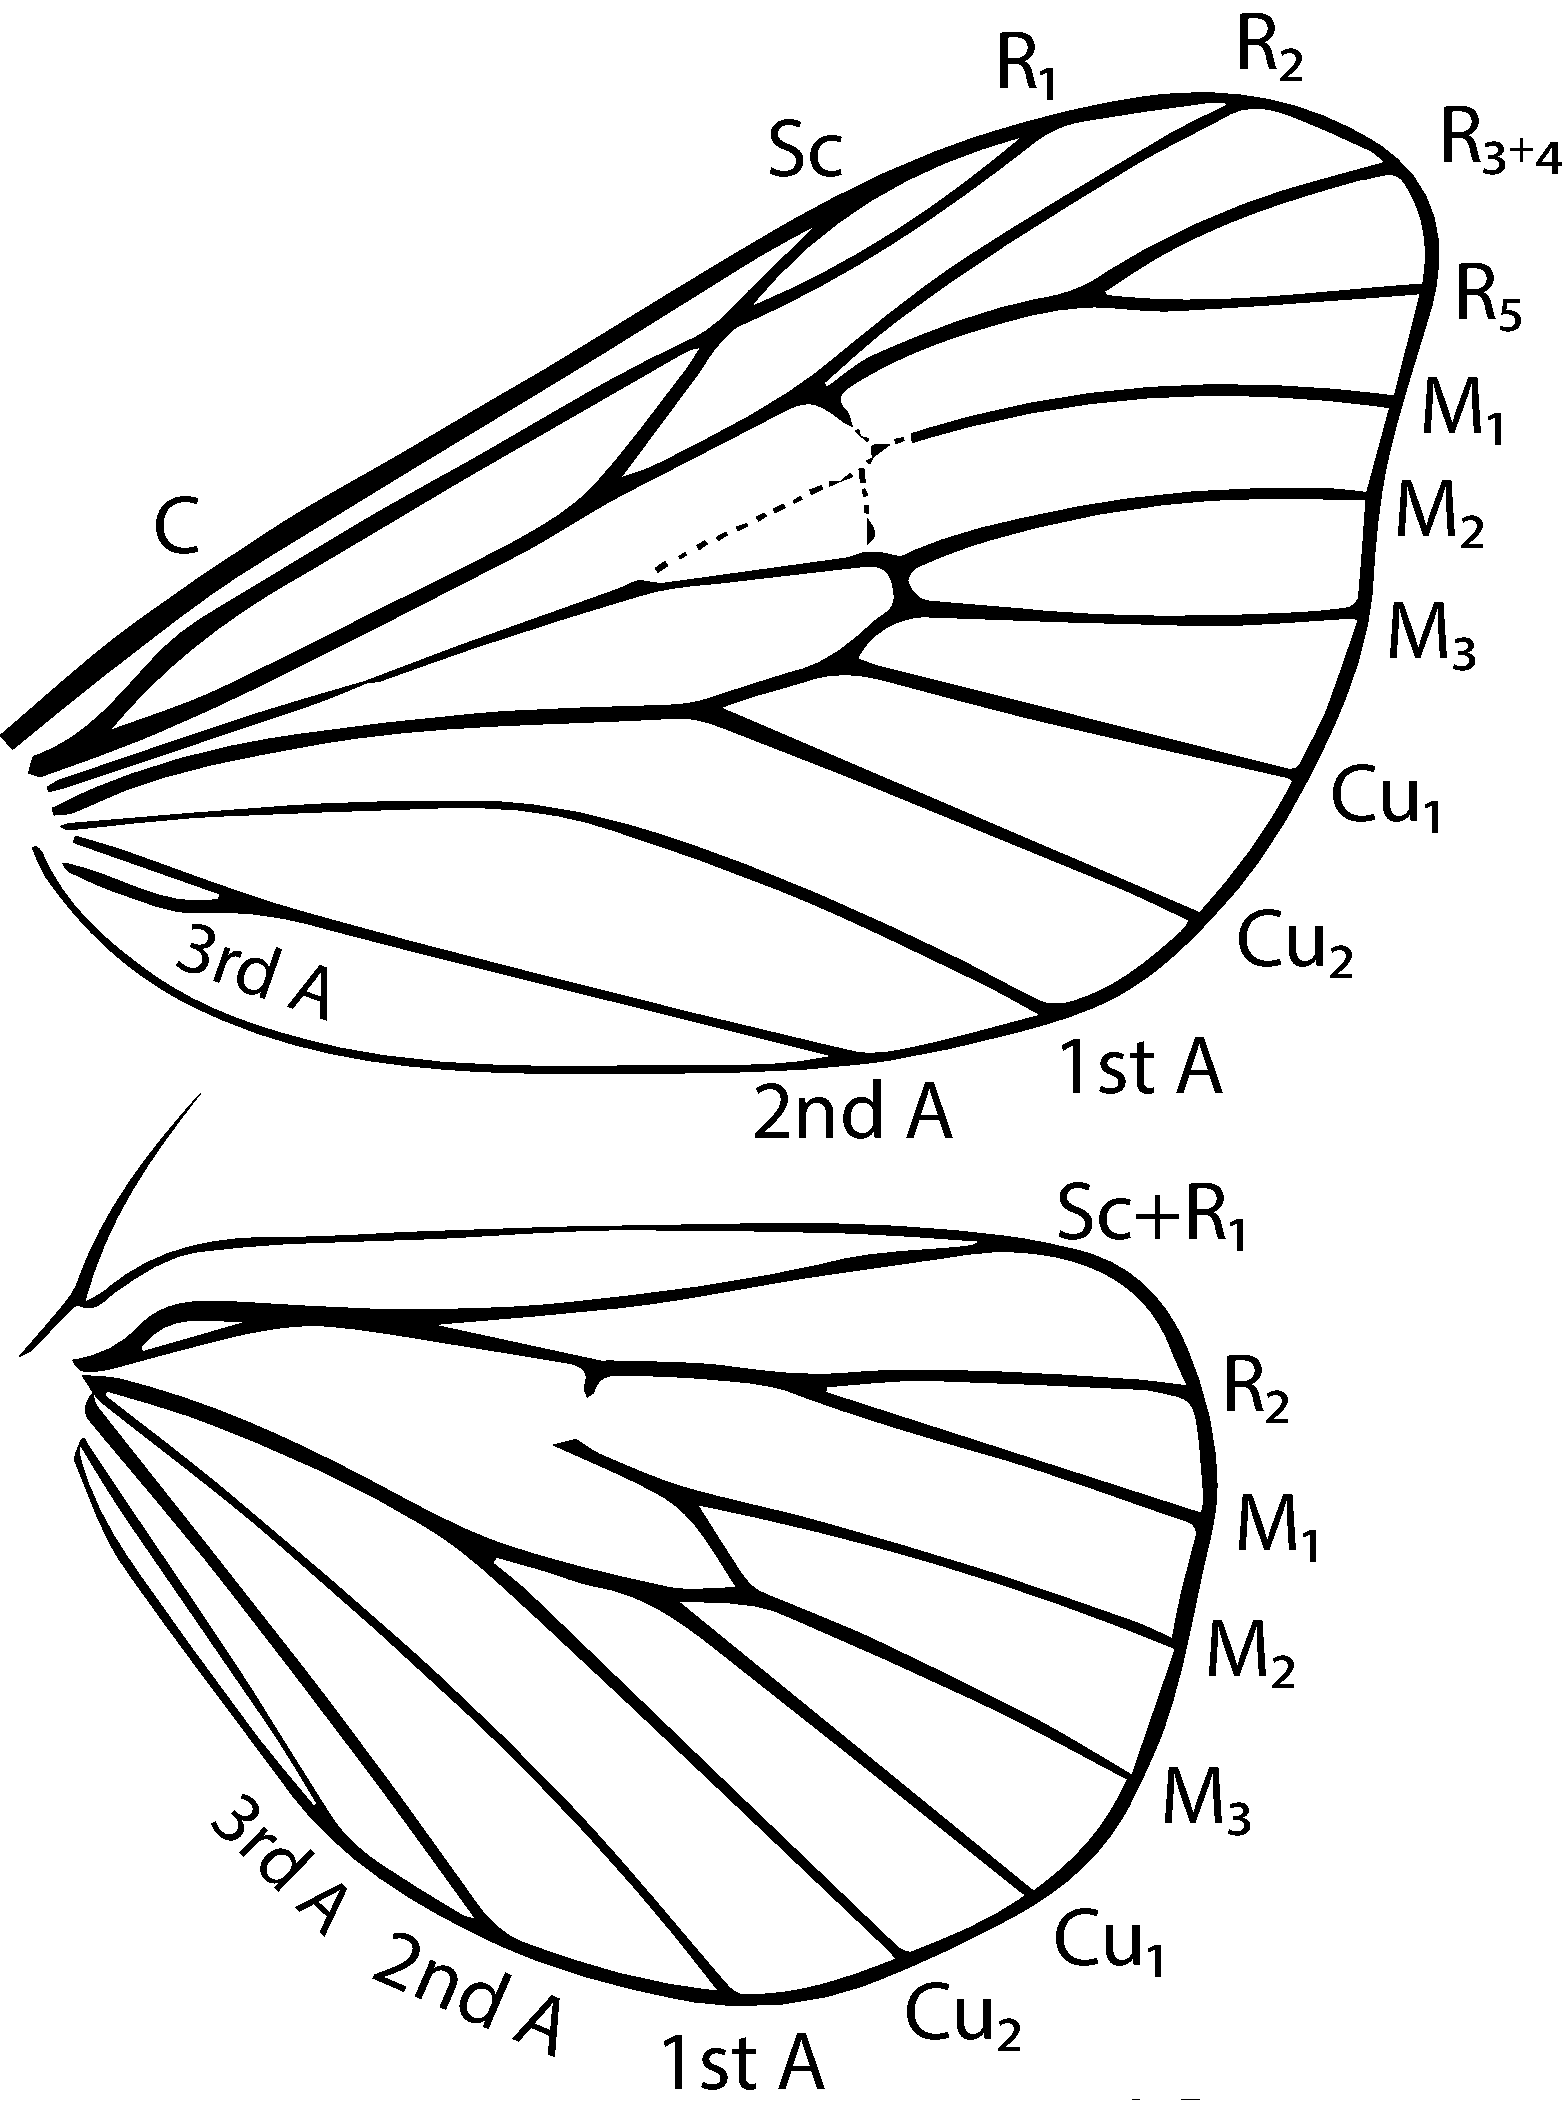
\includegraphics[width=\textwidth]{amphiesmenoptera/LimacodidWings}
        \caption{}
        \label{fig:limacodid1}
    \end{subfigure}
    \hfill 
    \begin{subfigure}[ht!]{0.55\textwidth}
        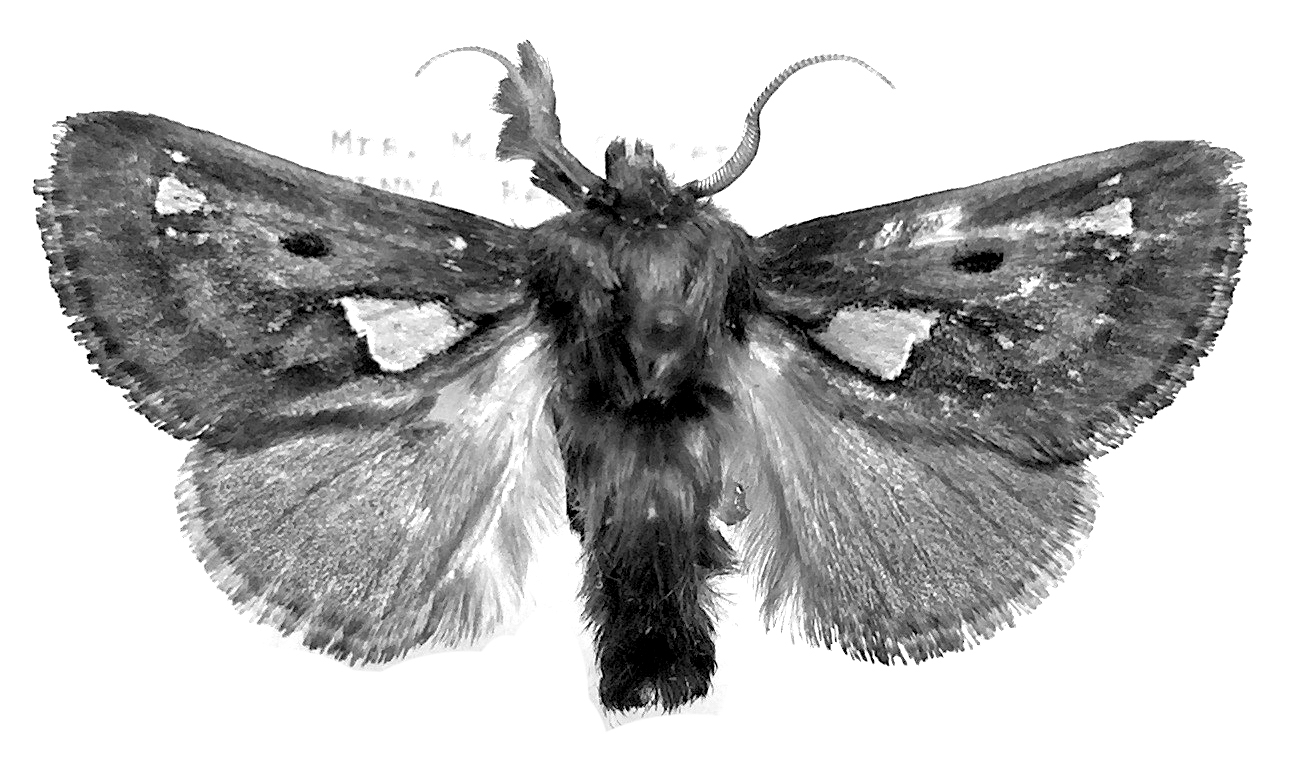
\includegraphics[width=\textwidth]{amphiesmenoptera/limacodid}
        \caption{}
        \label{fig:limacodid2}
    \end{subfigure}
    \caption{Limacodidae. \textbf{(a)} Wings \citep[Fig. 349]{comstock1918wings}; \textbf{(b)} habitus, photo (CC BY 2.0) by Andy Deans \url{https://flic.kr/p/FHd34h}}\label{fig:limacodids}
\end{figure}

\subsubsection{Pyraloidea (snout moths and relatives)}\index{Pyraloidea}
\noindent{}\textit{Diagnostic characters:} Fore wing usually elongate-triangular, hind wing more rounded and often broader (figure \ref{fig:pyraloids}); palps often large and projecting forward (figure \ref{fig:pyraloids}); proboscis scaly; tympana present on abdomen; Sc + R1 and Rs in hind wing fused beyond discal cell then separating (this character can be hard to see); hind wing with 3 anal veins.\vspace{3mm}

\noindent{}\textit{Natural history:} Large superfamily, with \textgreater{}15,000 described species and myriad life history strategies, including leaf miners, leaf rollers, borers, predators, coprophages, and aquatic species.\vspace{3mm}

\begin{theo}
{}We've seen a few taxa now that exhibit large palps. Given that these are liquid-feeders, what do you think are the function(s) of these structures?
\end{theo}

\begin{figure}[ht!]
    \centering
    \begin{subfigure}[ht!]{0.38\textwidth}
        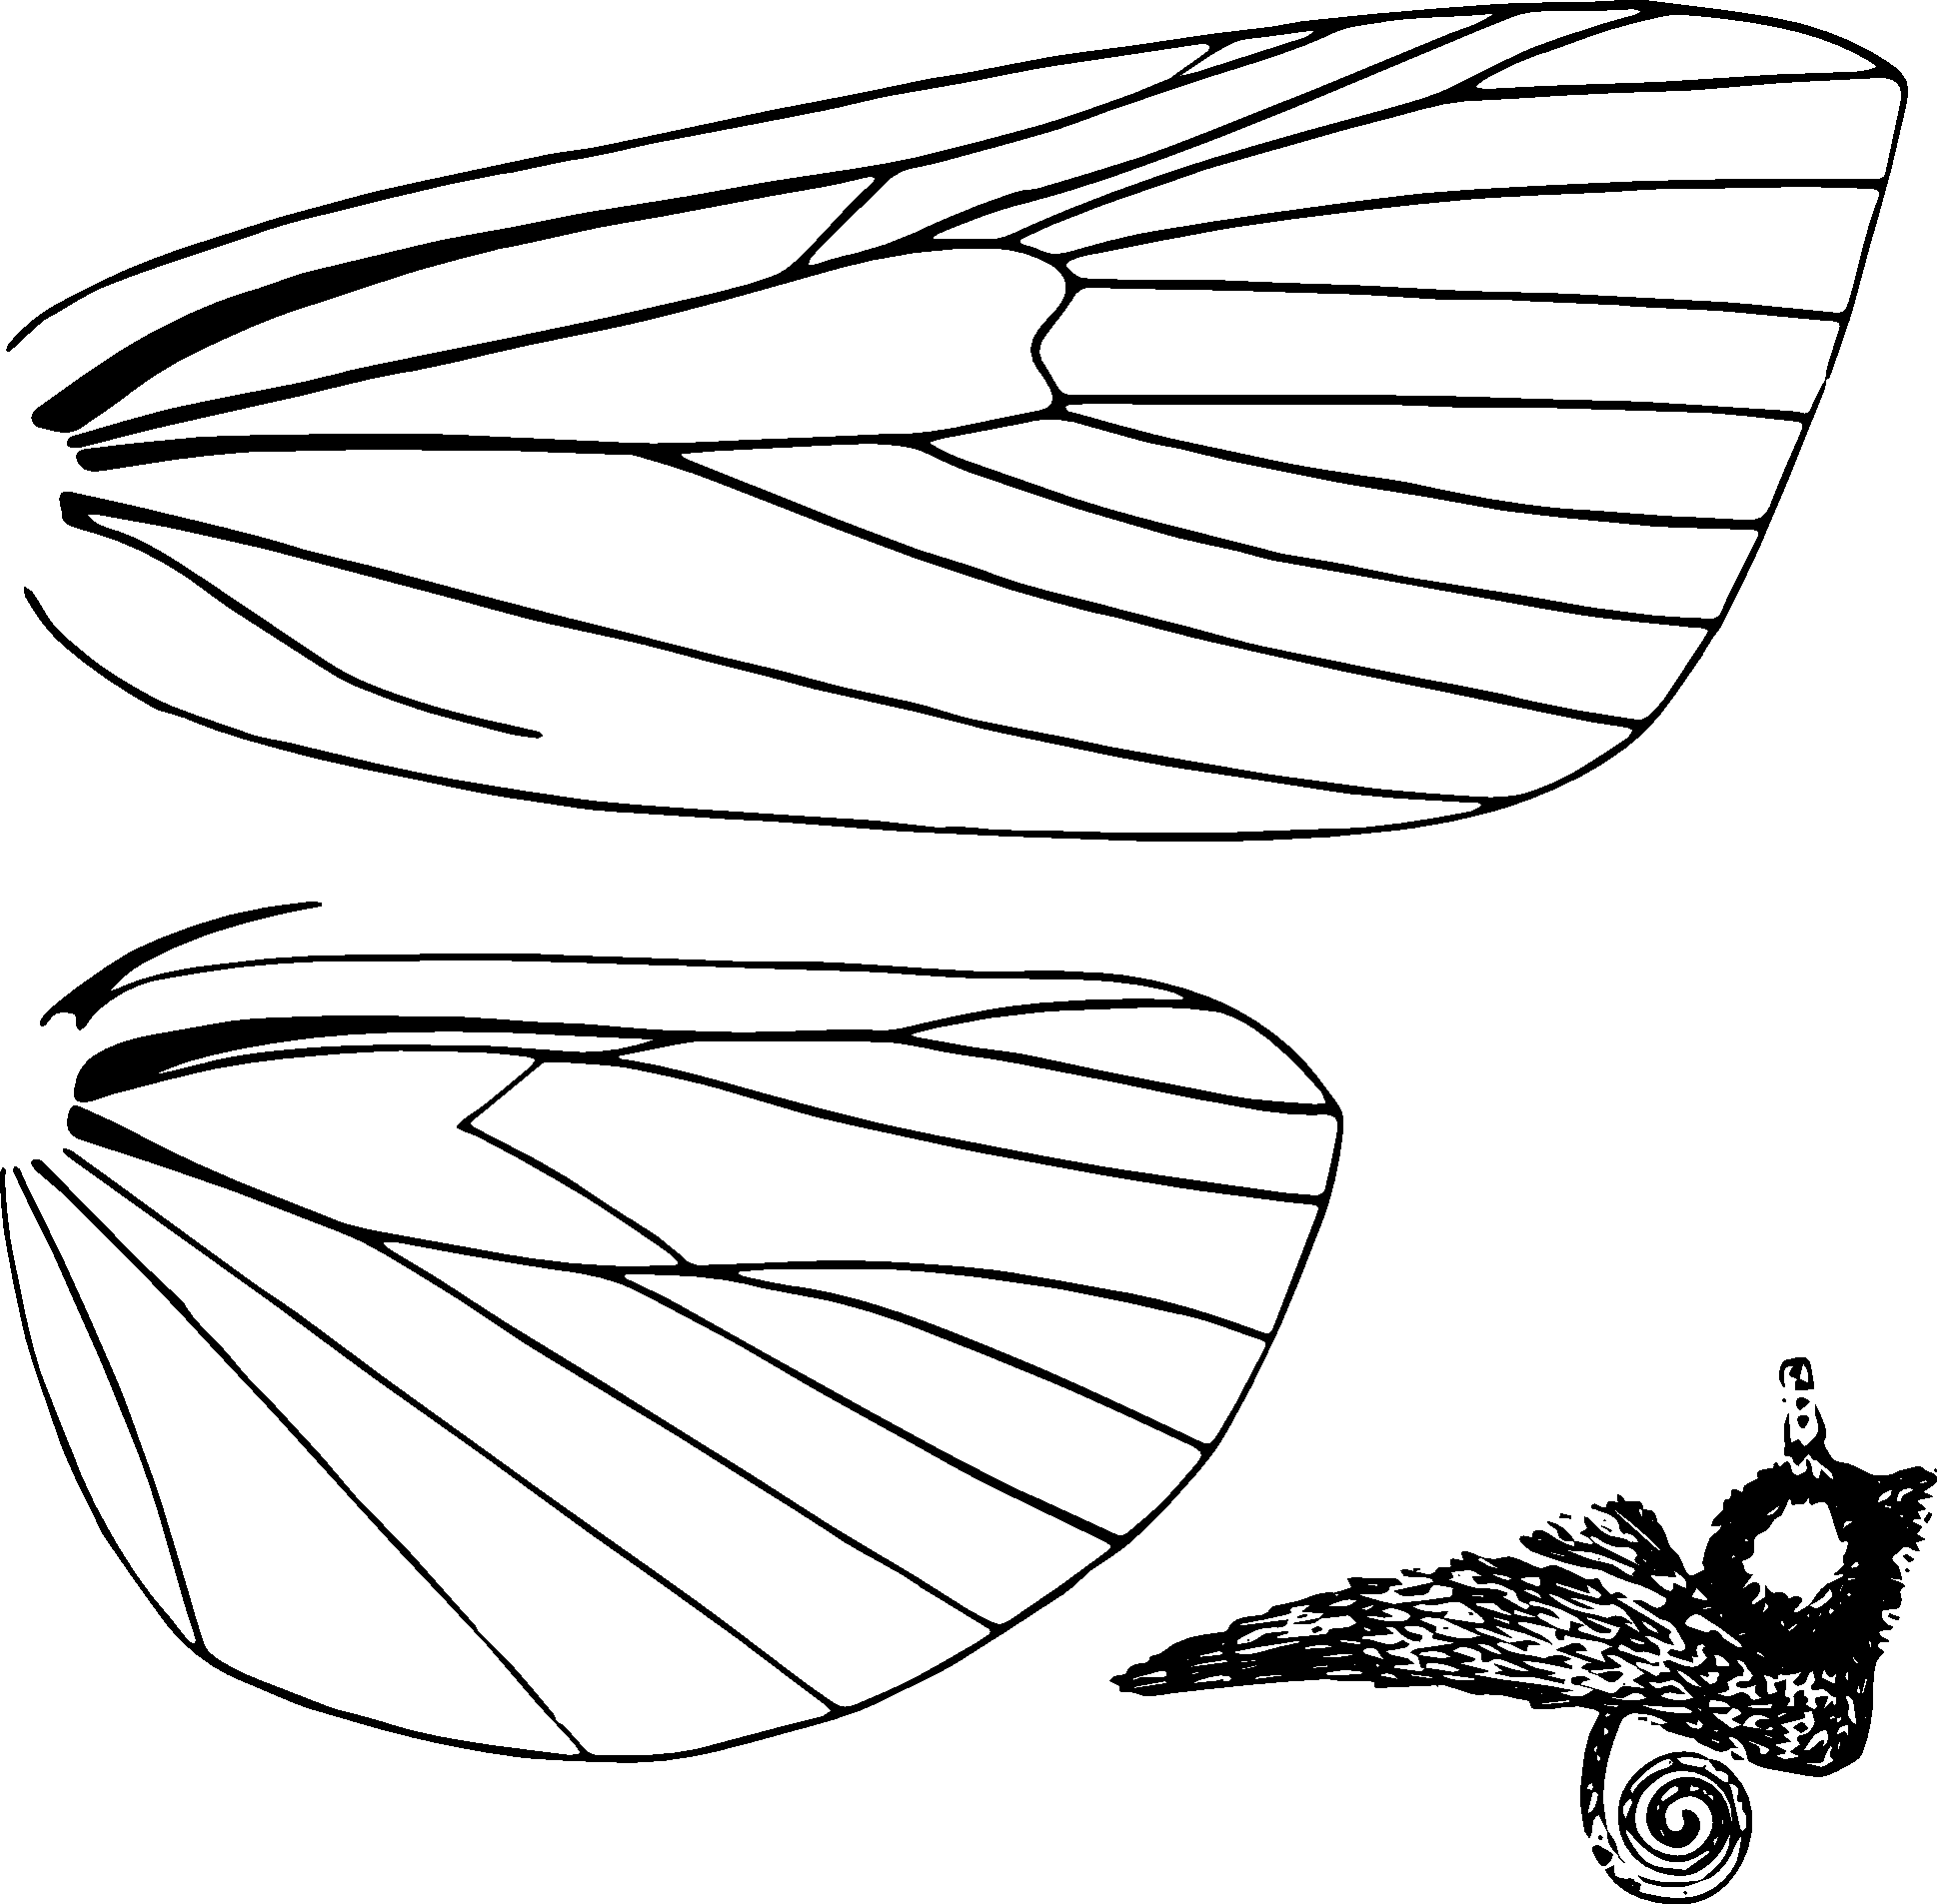
\includegraphics[width=\textwidth]{amphiesmenoptera/PyralidWings}
        \caption{}
        \label{fig:pyraloid1}
    \end{subfigure}
    \hfill 
    \begin{subfigure}[ht!]{0.55\textwidth}
        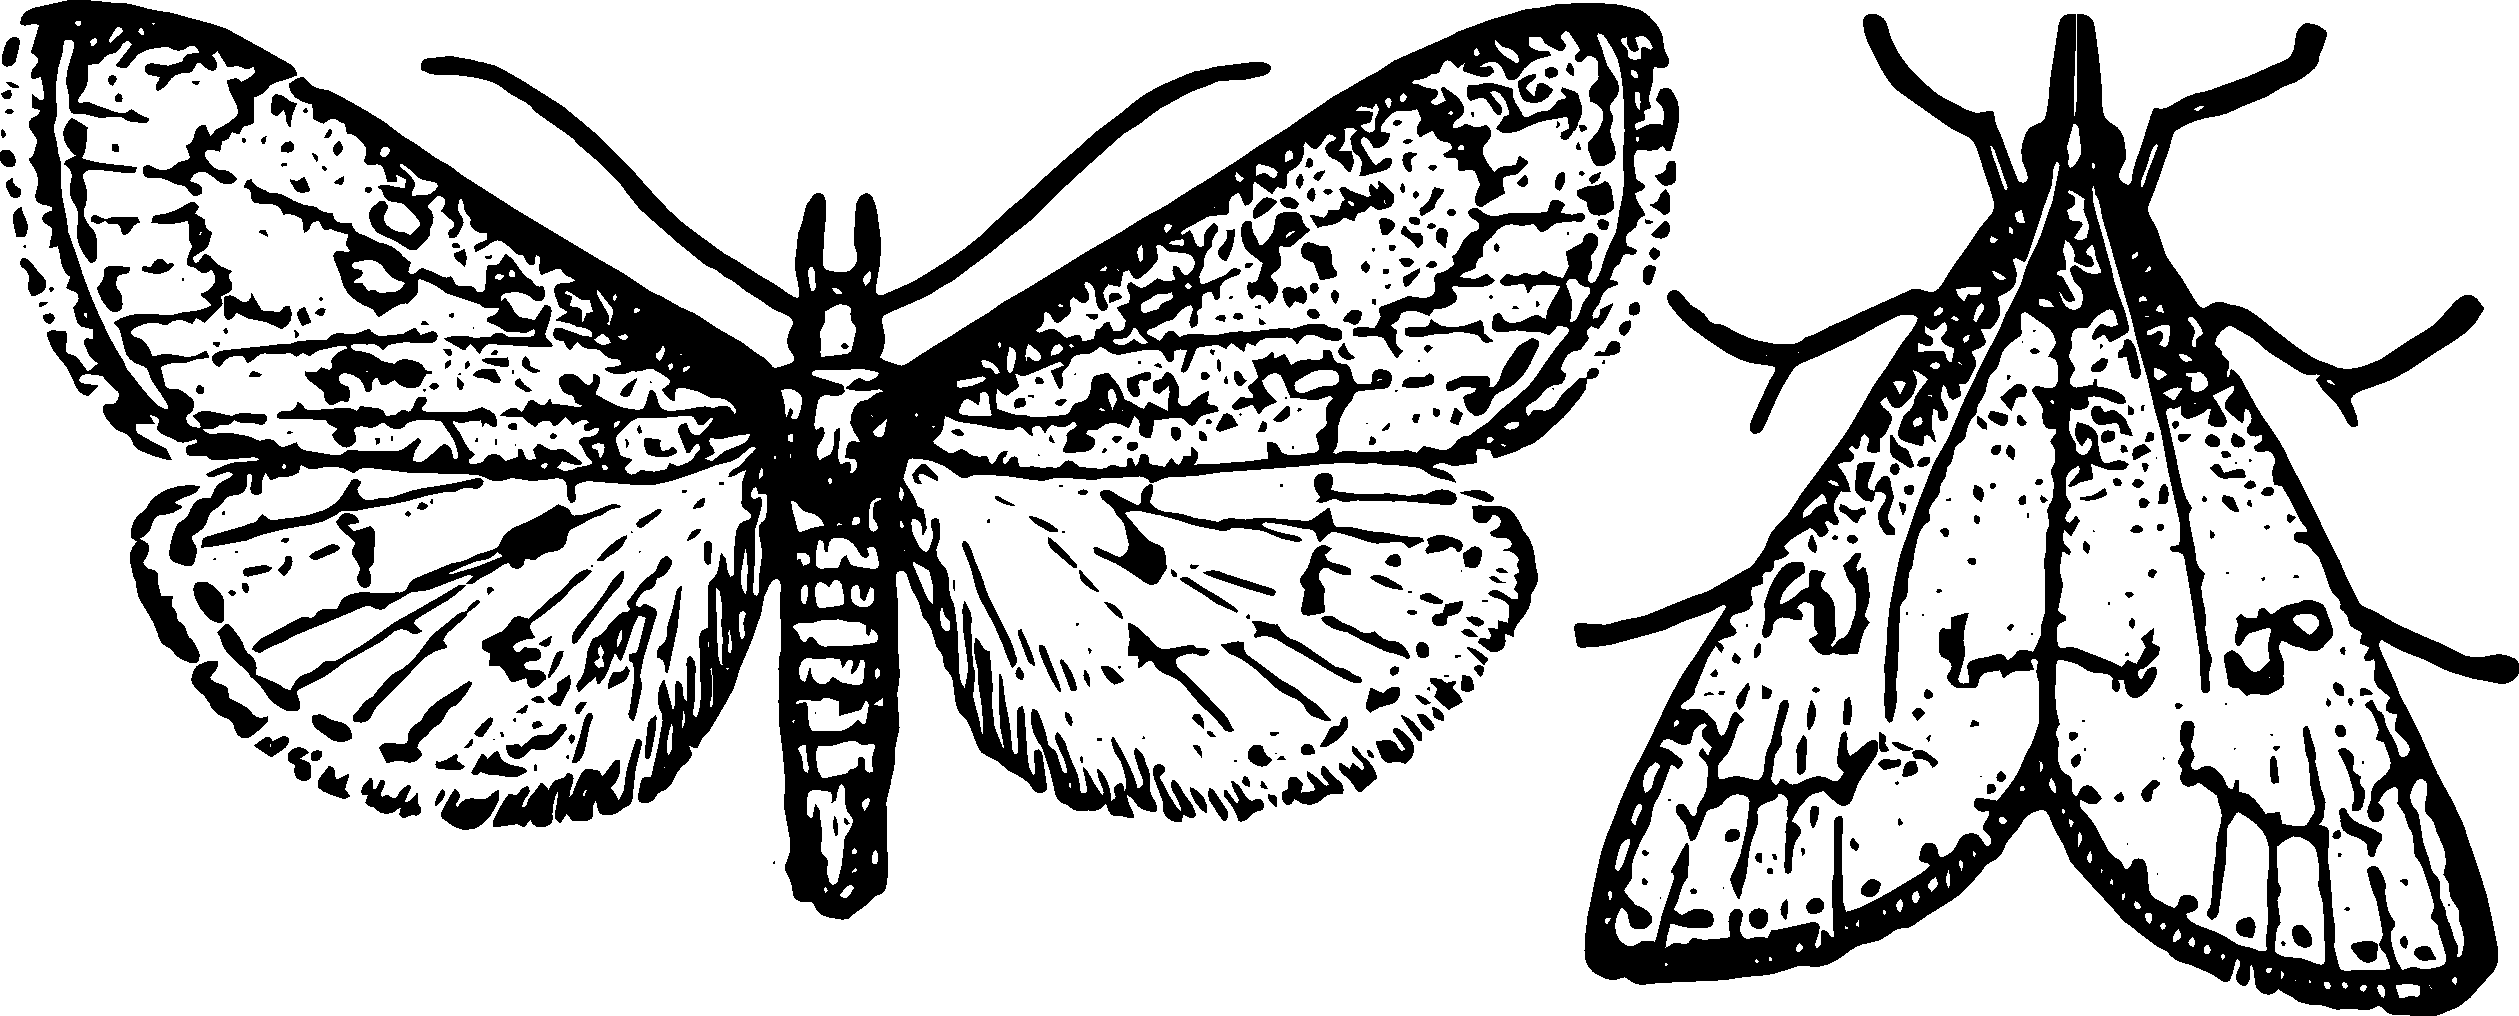
\includegraphics[width=\textwidth]{amphiesmenoptera/pyralids}
        \caption{}
        \label{fig:pyraloid2}
    \end{subfigure}
    \caption{Pyraloidea. \textbf{(a)} Wings \citep[][Plate C]{bhl73500}; \textbf{(b)} dorsal habitus \citep[][Fig. 296]{bhlitem92183}}\label{fig:pyraloids}
\end{figure}

\subsubsection{Geometridae (inchworms, spanworms, loopers, etc.)}\index{Geometridae}
\noindent{}\textit{Diagnostic characters:} Somewhat butterfly-like in shape, with broad wings; usually cryptically colored; geometric patterns on the fore wings often continue onto the hind wing (figure \ref{fig:geometrid2}); antennae thread-like or pectinate, not clubbed; proboscis bare; frenulum present, Sc in hind wing with an abrupt angle basally (arrow in figure \ref{fig:geometrid1}); tympana located at the base of the abdomen.\vspace{3mm}

\noindent{}\textit{Natural history:} Larvae often referred to as ``inchworms'', due to arched habitus and measured locomotion. More than 35,000 described species, including some in Hawai'i that are predators.\vspace{3mm}

\begin{figure}[ht!]
    \centering
    \begin{subfigure}[ht!]{0.26\textwidth}
        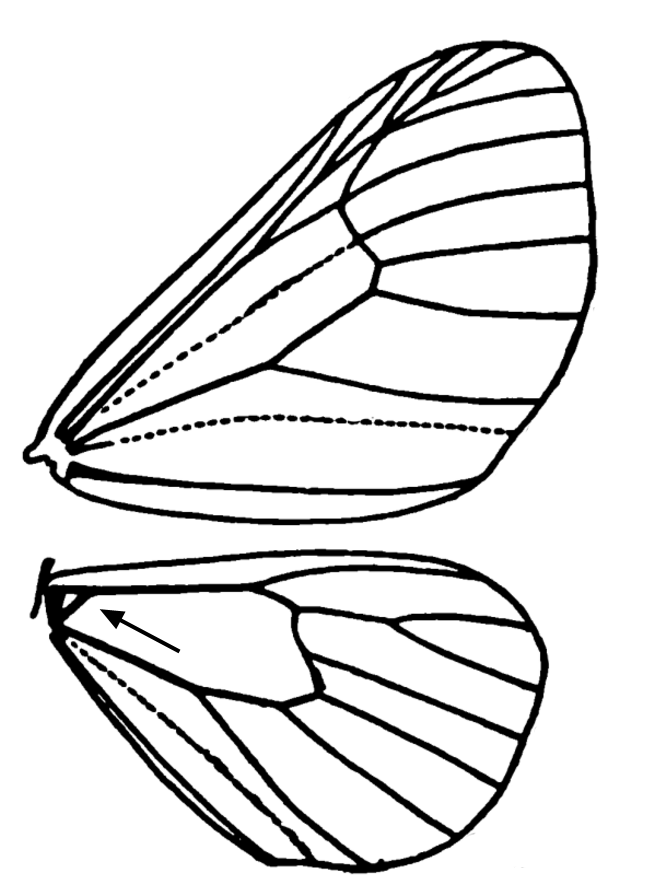
\includegraphics[width=\textwidth]{amphiesmenoptera/GeometridWings}
        \caption{}
        \label{fig:geometrid1}
    \end{subfigure}
    \hfill
    \begin{subfigure}[ht!]{0.54\textwidth}
        \includegraphics[width=\textwidth]{amphiesmenoptera/geometridHabitus}
        \caption{}
        \label{fig:geometrid2}
    \end{subfigure}
    \caption{Geometridae. \textbf{(a)} Wings \citep[][Fig. 20]{comstock1893evolution}; \textbf{(b)} habitus, redrawn from photo (CC0) by USDA Forest Service, Pacific Northwest Region \url{https://flic.kr/p/U4yVgL}}\label{fig:geometrids}
\end{figure}

%given the specimens you observed here in lab, what do you think is the sister to butterflies?

\FloatBarrier
\paragraph{Rhopalocera (butterflies)}\index{Rhopalocera} The next five families are all commonly referred to as butterflies (although Hesperiidae is sometimes excluded). They can be recognized by the following characters: antennae knobbed/hooked at tip; ocelli always absent; body usually small relative to wings, wings usually broad; hind wing with only 1 or 2 anal veins.

\subsubsection{Hesperiidae (skippers)}\index{Hesperiidae}
\noindent{}\textit{Diagnostic characters:} Antennae clubbed but also hooked at tip (figure \ref{fig:hesperiid1}); antennal insertions widely separated; R in fore wing 5-branched (figure \ref{fig:hesperiid1}); fairly stout-bodied compared to butterflies, with large, broad heads (figure \ref{fig:hesperiid2}).\vspace{3mm}

\noindent{}\textit{Natural history:} More than 3,500 species described worldwide. Larvae often live in shelters, \textit{e.g.} leaf rolls, they construct for themselves. Adults are diurnal and have a characteristic darting flight.

\begin{figure}[ht!]
    \centering
    \begin{subfigure}[ht!]{0.36\textwidth}
        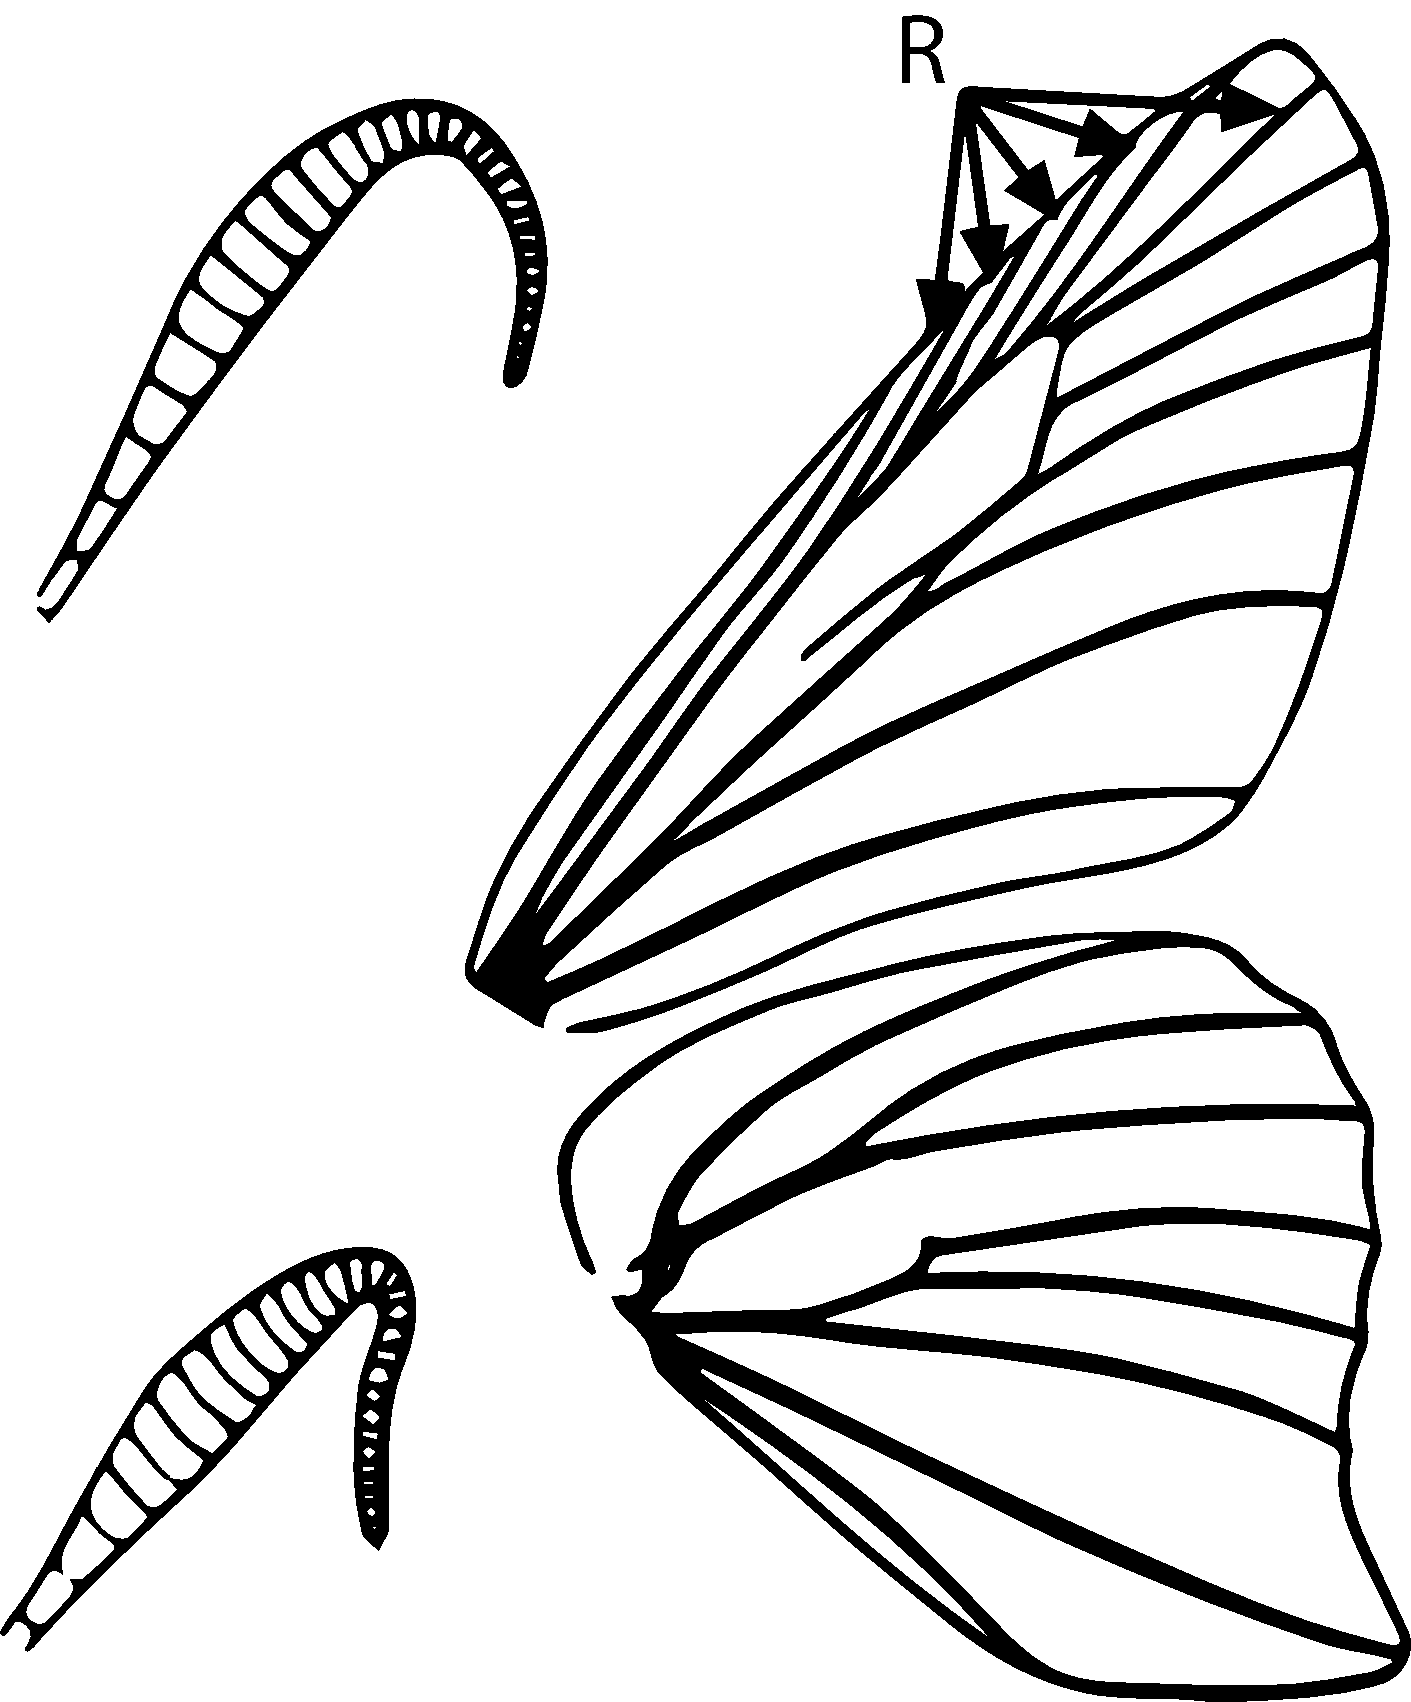
\includegraphics[width=\textwidth]{amphiesmenoptera/HesperiidWings}
        \caption{}
        \label{fig:hesperiid1}
    \end{subfigure}
    \hfill
    \begin{subfigure}[ht!]{0.55\textwidth}
        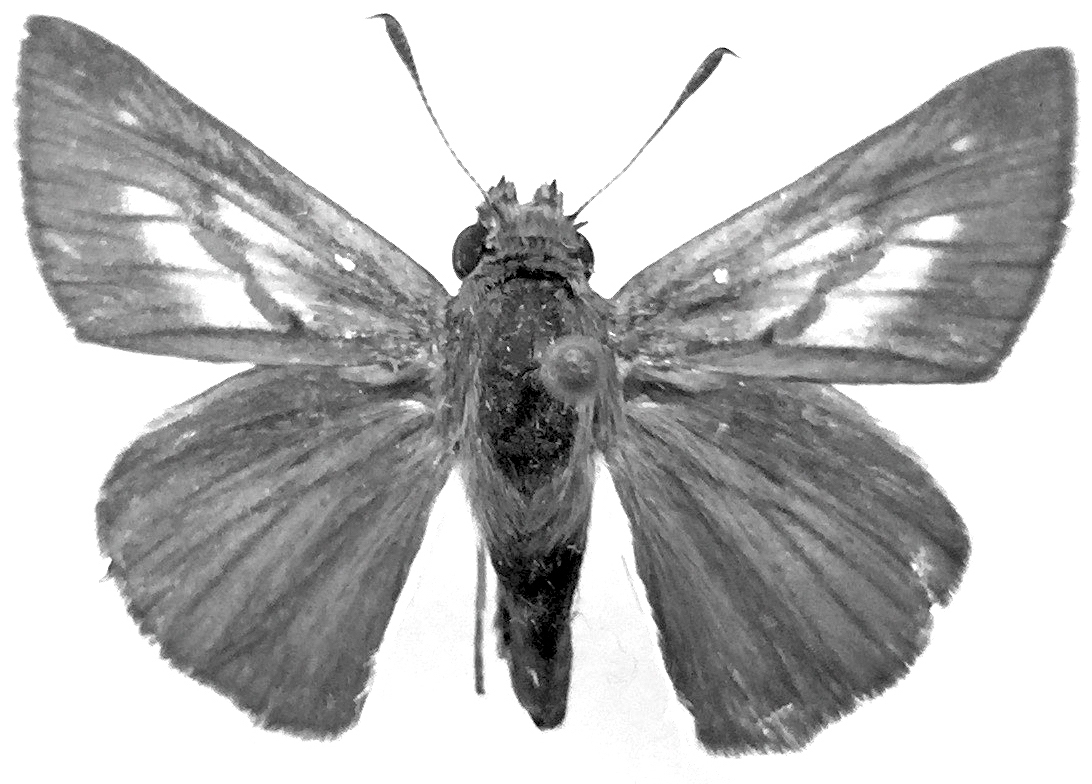
\includegraphics[width=\textwidth]{amphiesmenoptera/hesperiid}
        \caption{}
        \label{fig:hesperiid2}
    \end{subfigure}
    \caption{Hesperiidae. \textbf{(a)} Wings (right) and apical flagellomeres (left) \citep[][Fig. 5]{bhl37915}; \textbf{(b)} habitus, photo (CC BY 2.0) by Andy Deans \url{https://flic.kr/p/G2taKT}}\label{fig:hesperiids}
\end{figure}

\subsubsection{Papilionidae (swallowtails)}\index{Papilionidae}
\noindent{}\textit{Diagnostic characters:} Fore wing with R 5-branched; hind wing with 1 anal vein and usually with tail-like projection (figure \ref{fig:papilionid1}); 4 branches off Cu at bottom of discal cell; fore legs not reduced; usually brightly colored (black, yellow and other colors) (figure \ref{fig:papilionid2}) and large.\vspace{3mm}

\noindent{}\textit{Natural history:} More than 550 species worldwide, including the largest butterflies (the birdwings (Troidini) of southeast Asia). Larvae, which often mimic snakes, have a forked, defensive evagination (osmeterium) that can be exserted from behind the head.\vspace{3mm}

\begin{figure}[ht!]
    \centering
    \begin{subfigure}[ht!]{0.28\textwidth}
        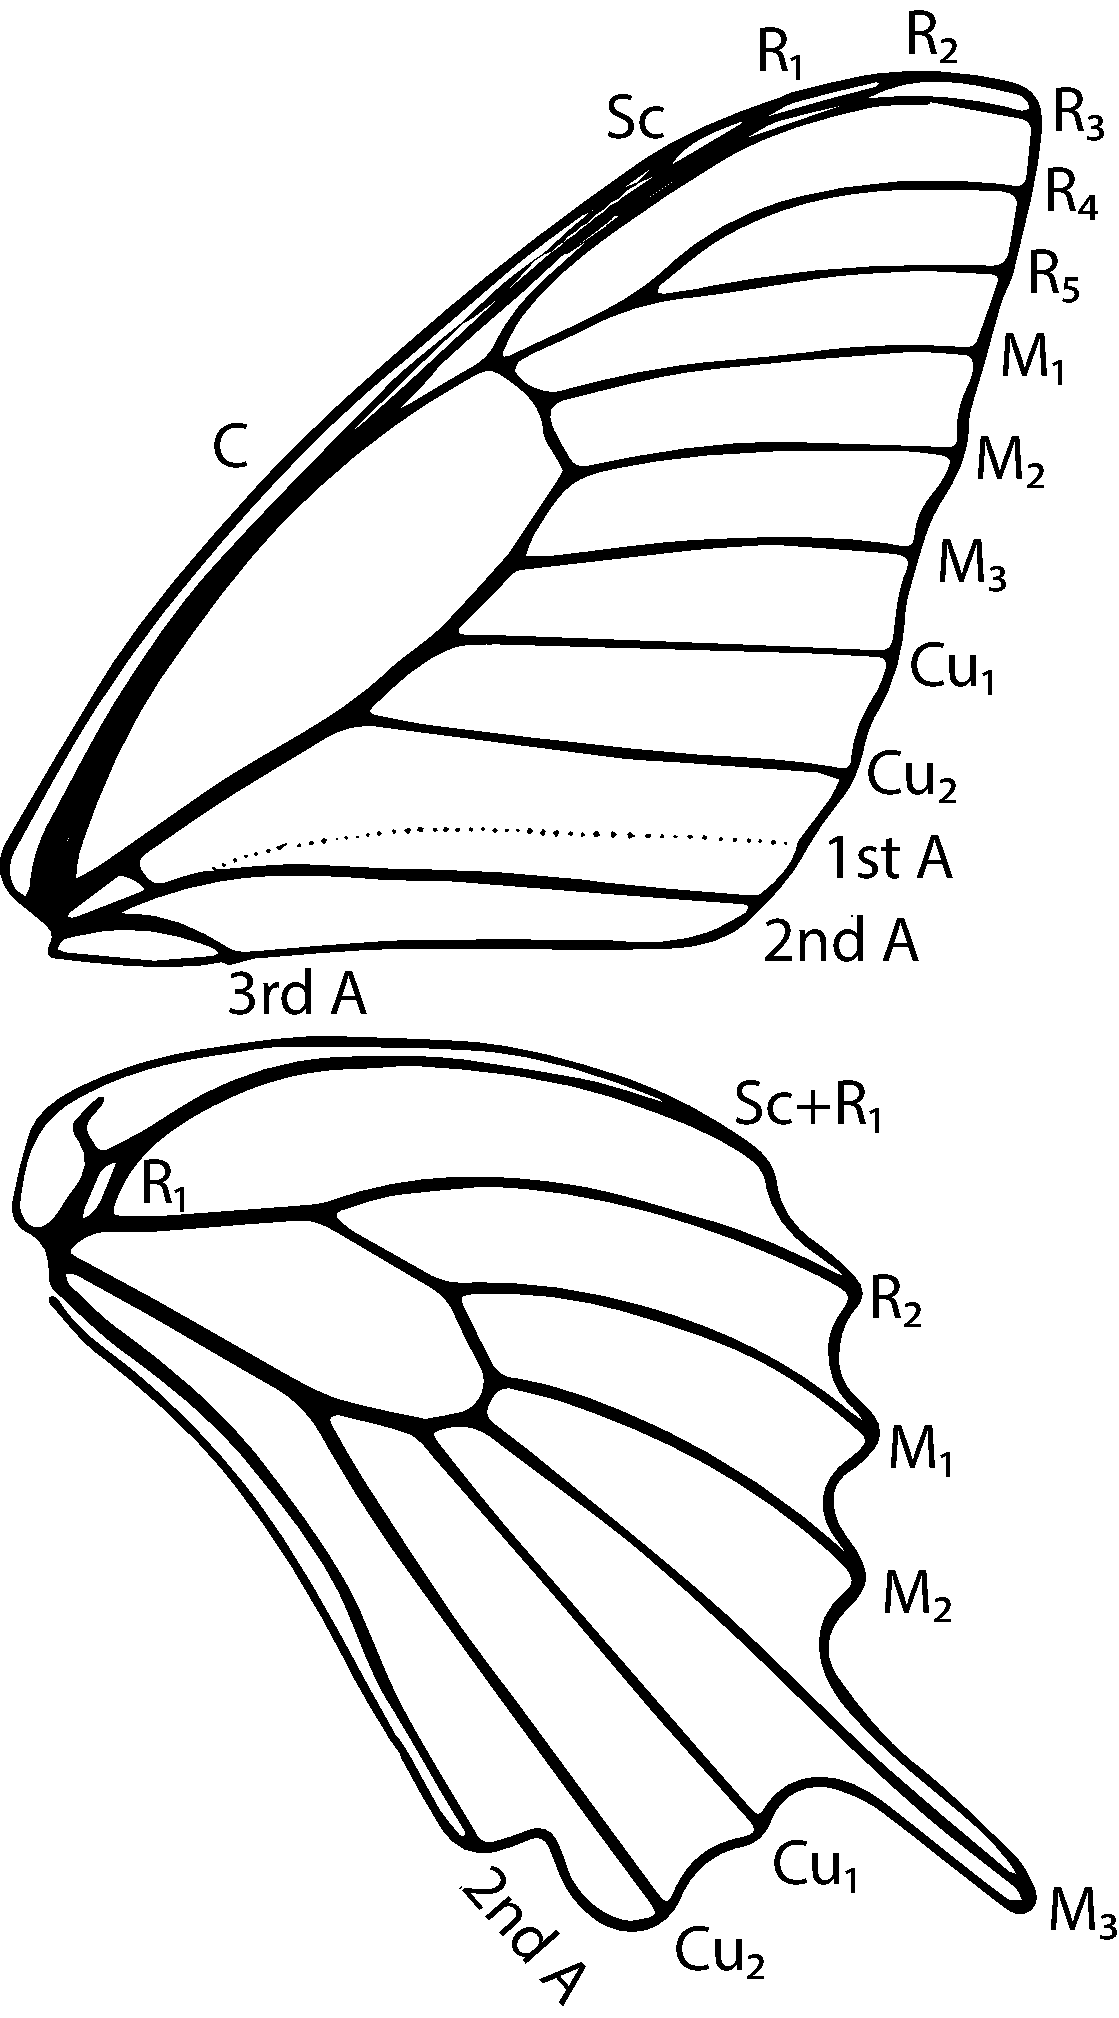
\includegraphics[width=\textwidth]{amphiesmenoptera/PapilionidWings}
        \caption{}
        \label{fig:papilionid1}
    \end{subfigure}
    \hfill 
    \begin{subfigure}[ht!]{0.6\textwidth}
        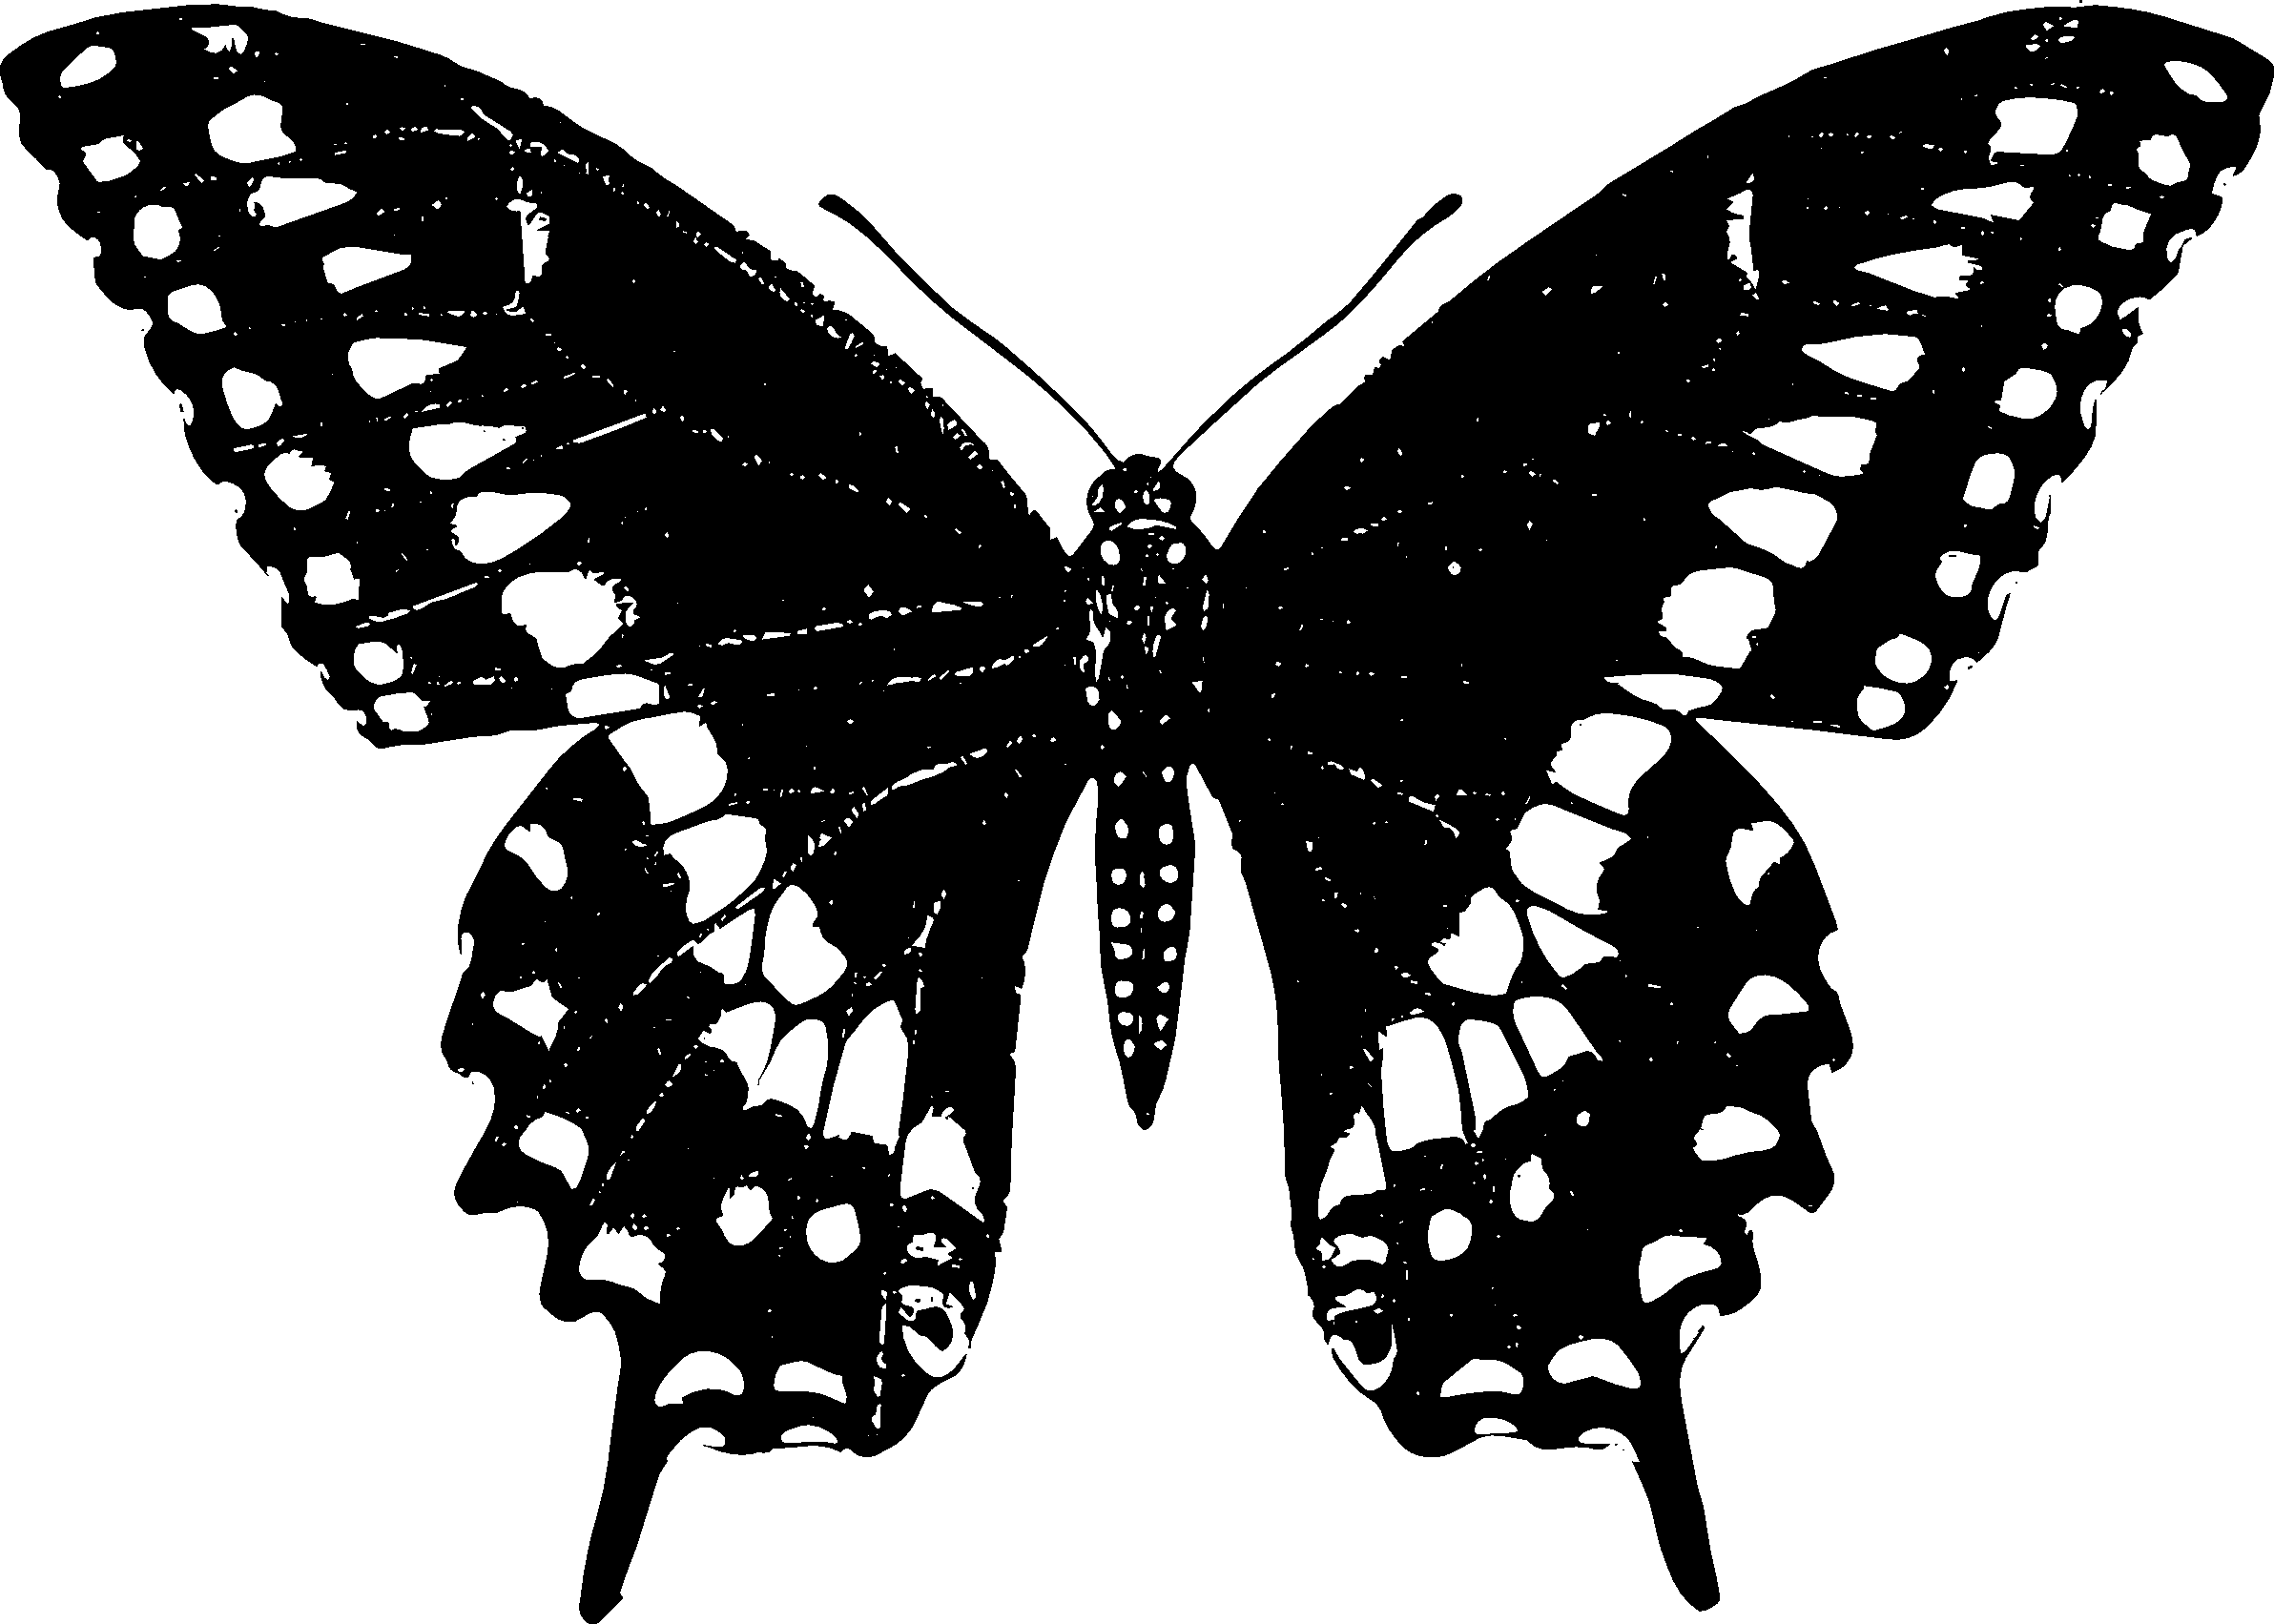
\includegraphics[width=\textwidth]{amphiesmenoptera/papilionid}
        \caption{}
        \label{fig:papilionid2}
    \end{subfigure}
    \caption{Papilionidae. \textbf{(a)} Wings \citep[Fig. 350]{comstock1918wings}; \textbf{(b)} habitus \citep[modified from][Fig. 317]{bhlitem38199}}\label{fig:papilionids}
\end{figure}

\subsubsection{Nymphalidae (brush-footed butterflies)}\index{Nymphalidae}
\noindent{}\textit{Diagnostic characters:} Body size diverse; wings variable in color and shape; R 5-branched in fore wing (figure \ref{fig:nymphalid1}); discal cell in hind wing often open or weakly closed; fore legs greatly reduced, lacking tarsal claws (rarely normal sized).\vspace{3mm}

\noindent{}\textit{Natural history:} With more than 6,000 known species this is the largest family of butterflies; includes monarchs, satyrs, morphos, fritillaries, commas, and many other recognizable butterflies.

\begin{figure}[ht!]
    \centering
    \begin{subfigure}[ht!]{0.25\textwidth}
        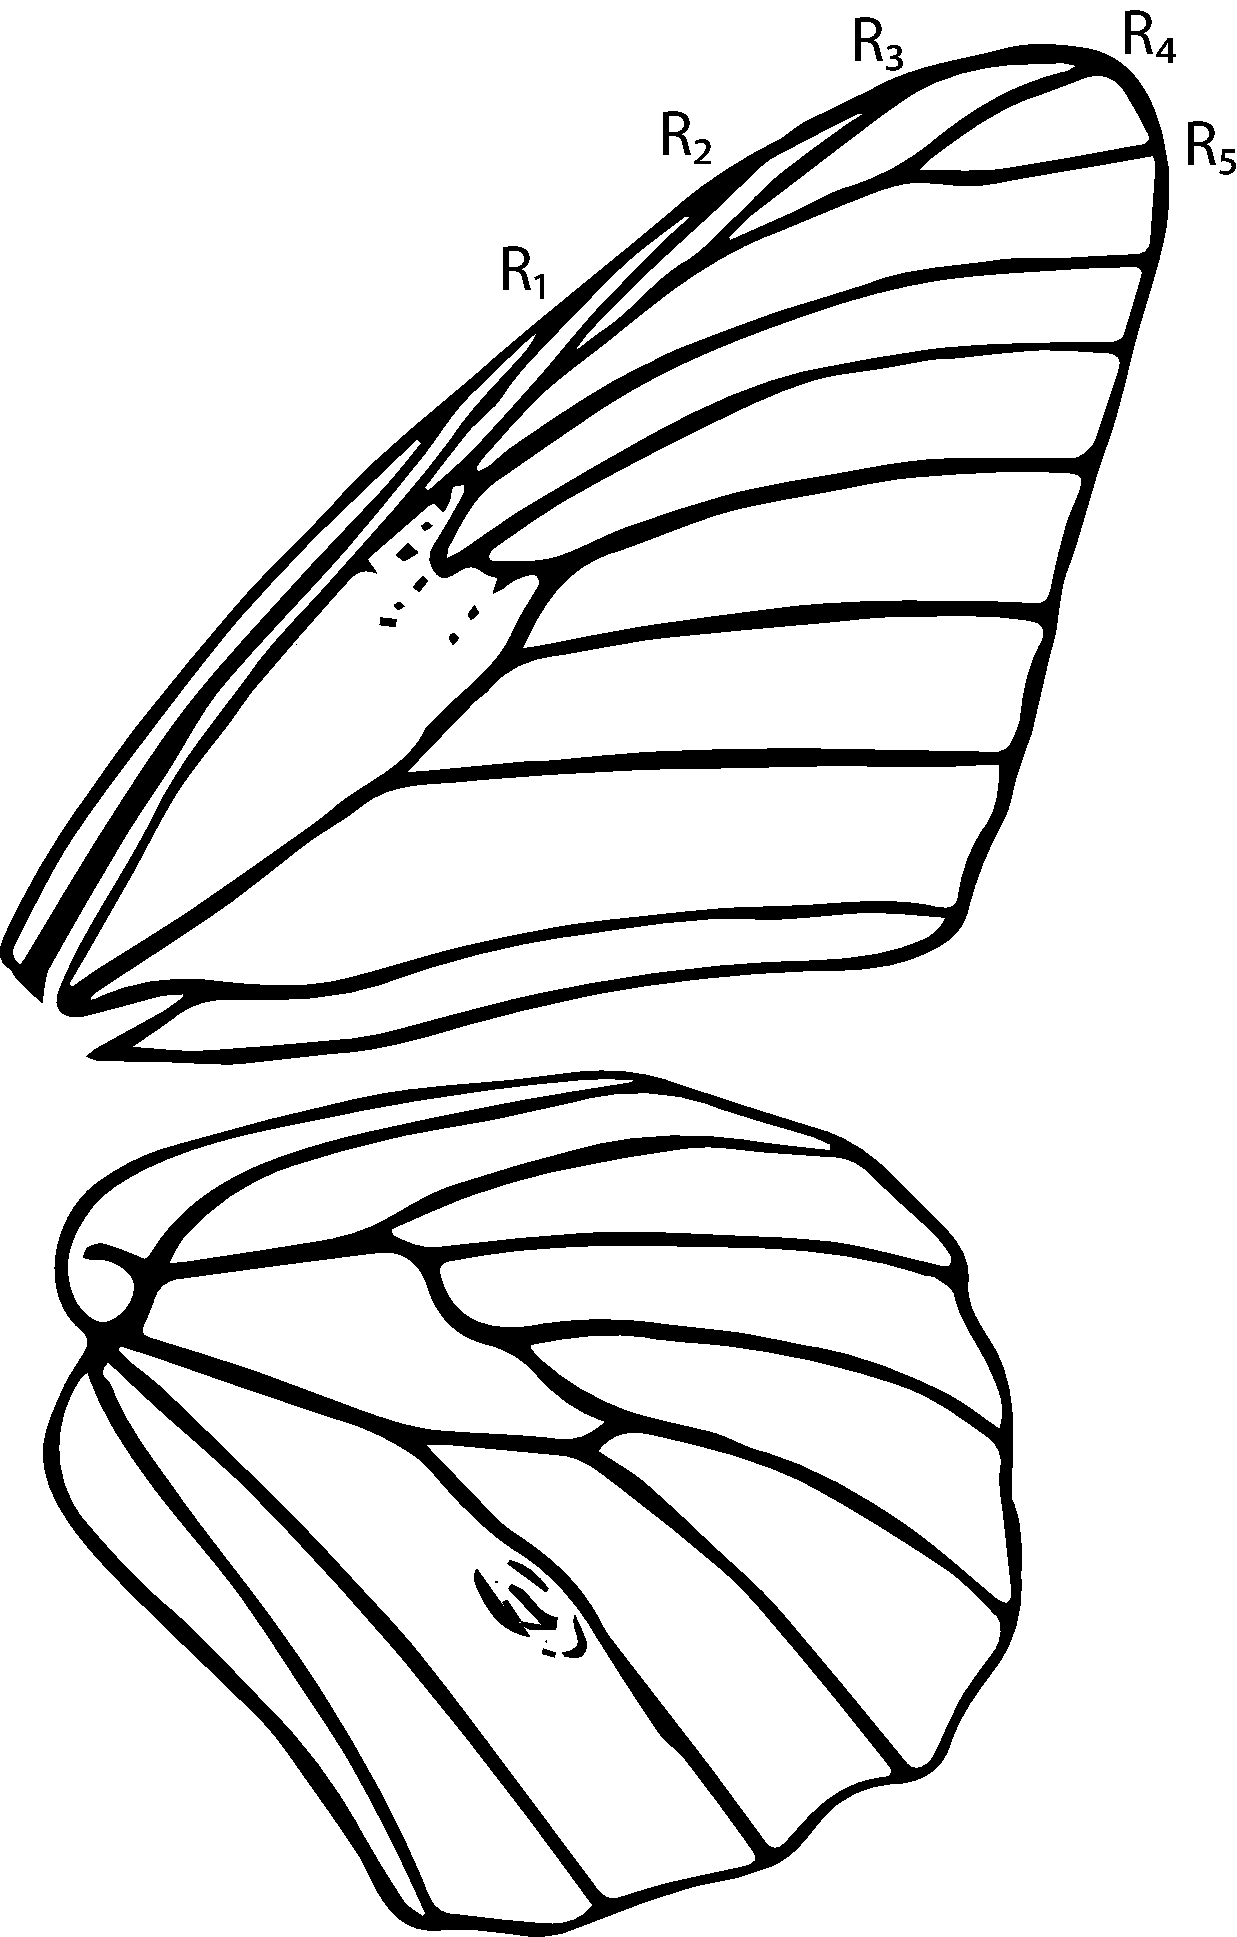
\includegraphics[width=\textwidth]{amphiesmenoptera/NymphalidWings}
        \caption{}
        \label{fig:nymphalid1}
    \end{subfigure}
    \hfill
    \begin{subfigure}[ht!]{0.30\textwidth}
        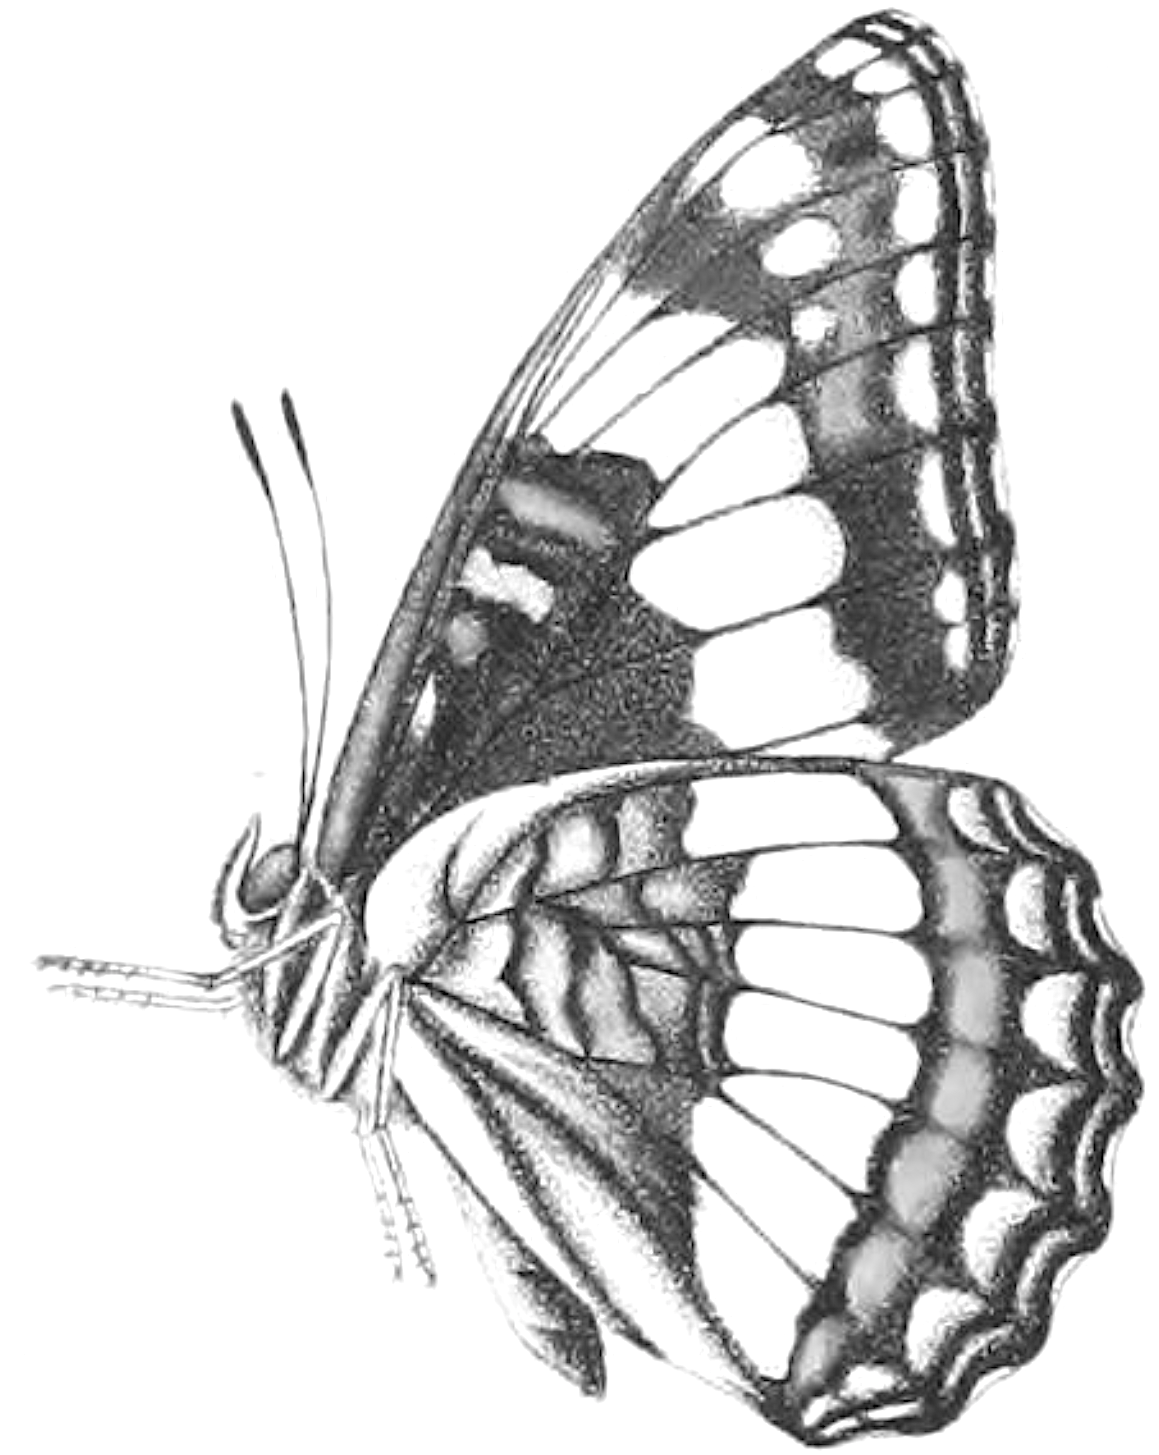
\includegraphics[width=\textwidth]{amphiesmenoptera/nymphalidLateral}
        \caption{}
        \label{fig:nymphalid2}
    \end{subfigure}
        \hfill
    \begin{subfigure}[ht!]{0.38\textwidth}
        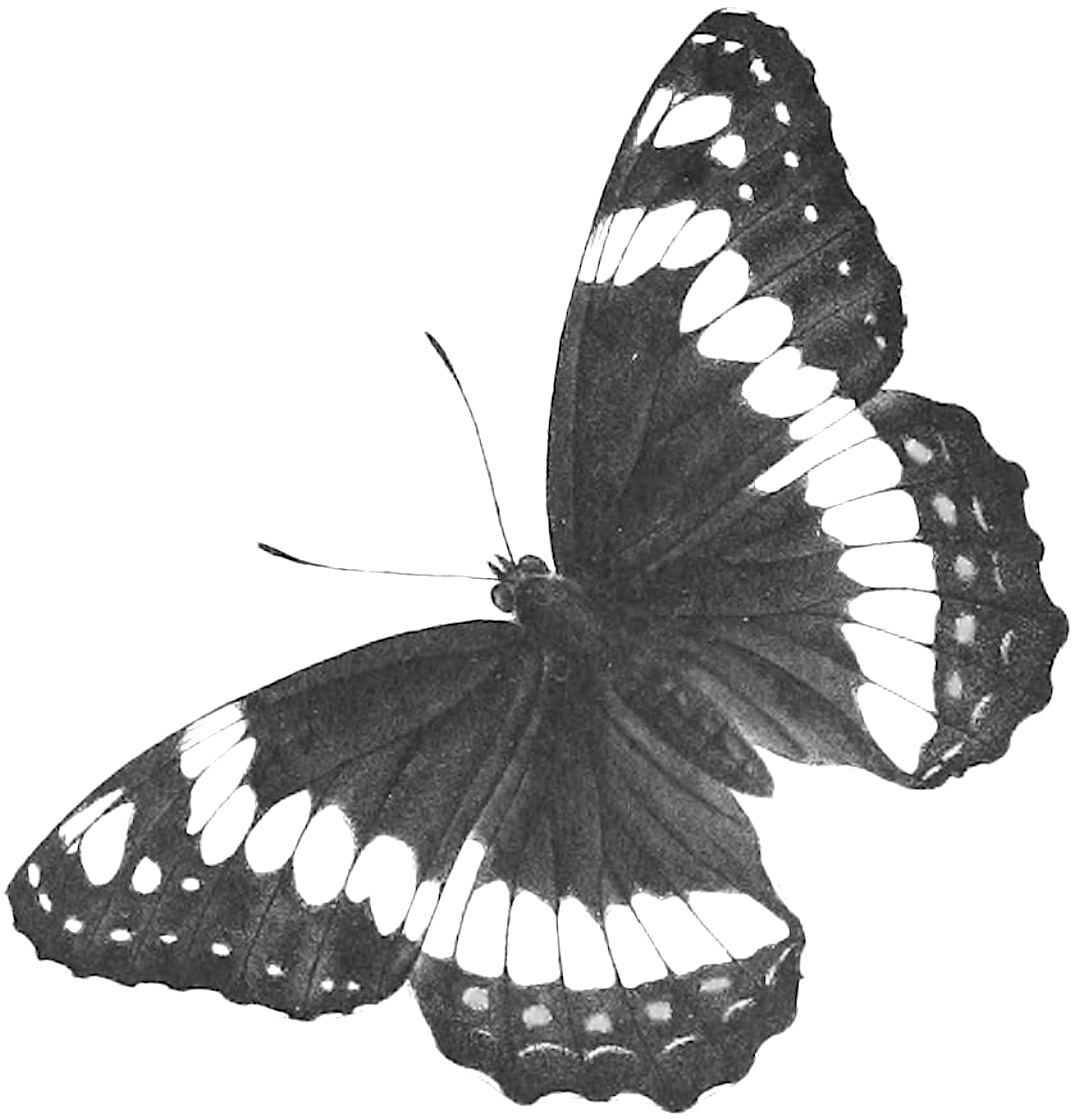
\includegraphics[width=\textwidth]{amphiesmenoptera/nymphalidDorsal}
        \caption{}
        \label{fig:nymphalid3}
    \end{subfigure}
    \caption{Nymphalidae. \textbf{(a)} Wings \citep[][Fig. 78]{bhl162310}; \textbf{(b)} lateral habitus \citep[Modified from Limenitis II in][]{bhlitem37427butt}; \textbf{(c)} dorsal habitus \citep[Modified from Limenitis II in][]{bhlitem37427butt}}\label{fig:nymphalids}
\end{figure}

\subsubsection{Pieridae (whites and sulfurs)}\index{Pieridae}
\noindent{}\textit{Diagnostic characters:} Medium sized (wingspan mostly 40--60 mm) and usually white, yellow, or orange, often marked with black (figure \ref{fig:pierid2}); fore wing R 3--5-branched; M1 of fore wing stalked with a branch of R near wing tip; hind wing with 2 anal veins and no tail (figure \ref{fig:pierid1}); front legs not or only slightly reduced; tarsal claws bifid.\vspace{3mm}

\noindent{}\textit{Natural history:} Approximately 1,100 species described worldwide. They feed on a diversity of plants, especially Brassicaceae and Fabaceae, and many species are migratory.\vspace{3mm}

\begin{figure}[ht!]
    \centering
    \begin{subfigure}[ht!]{0.25\textwidth}
        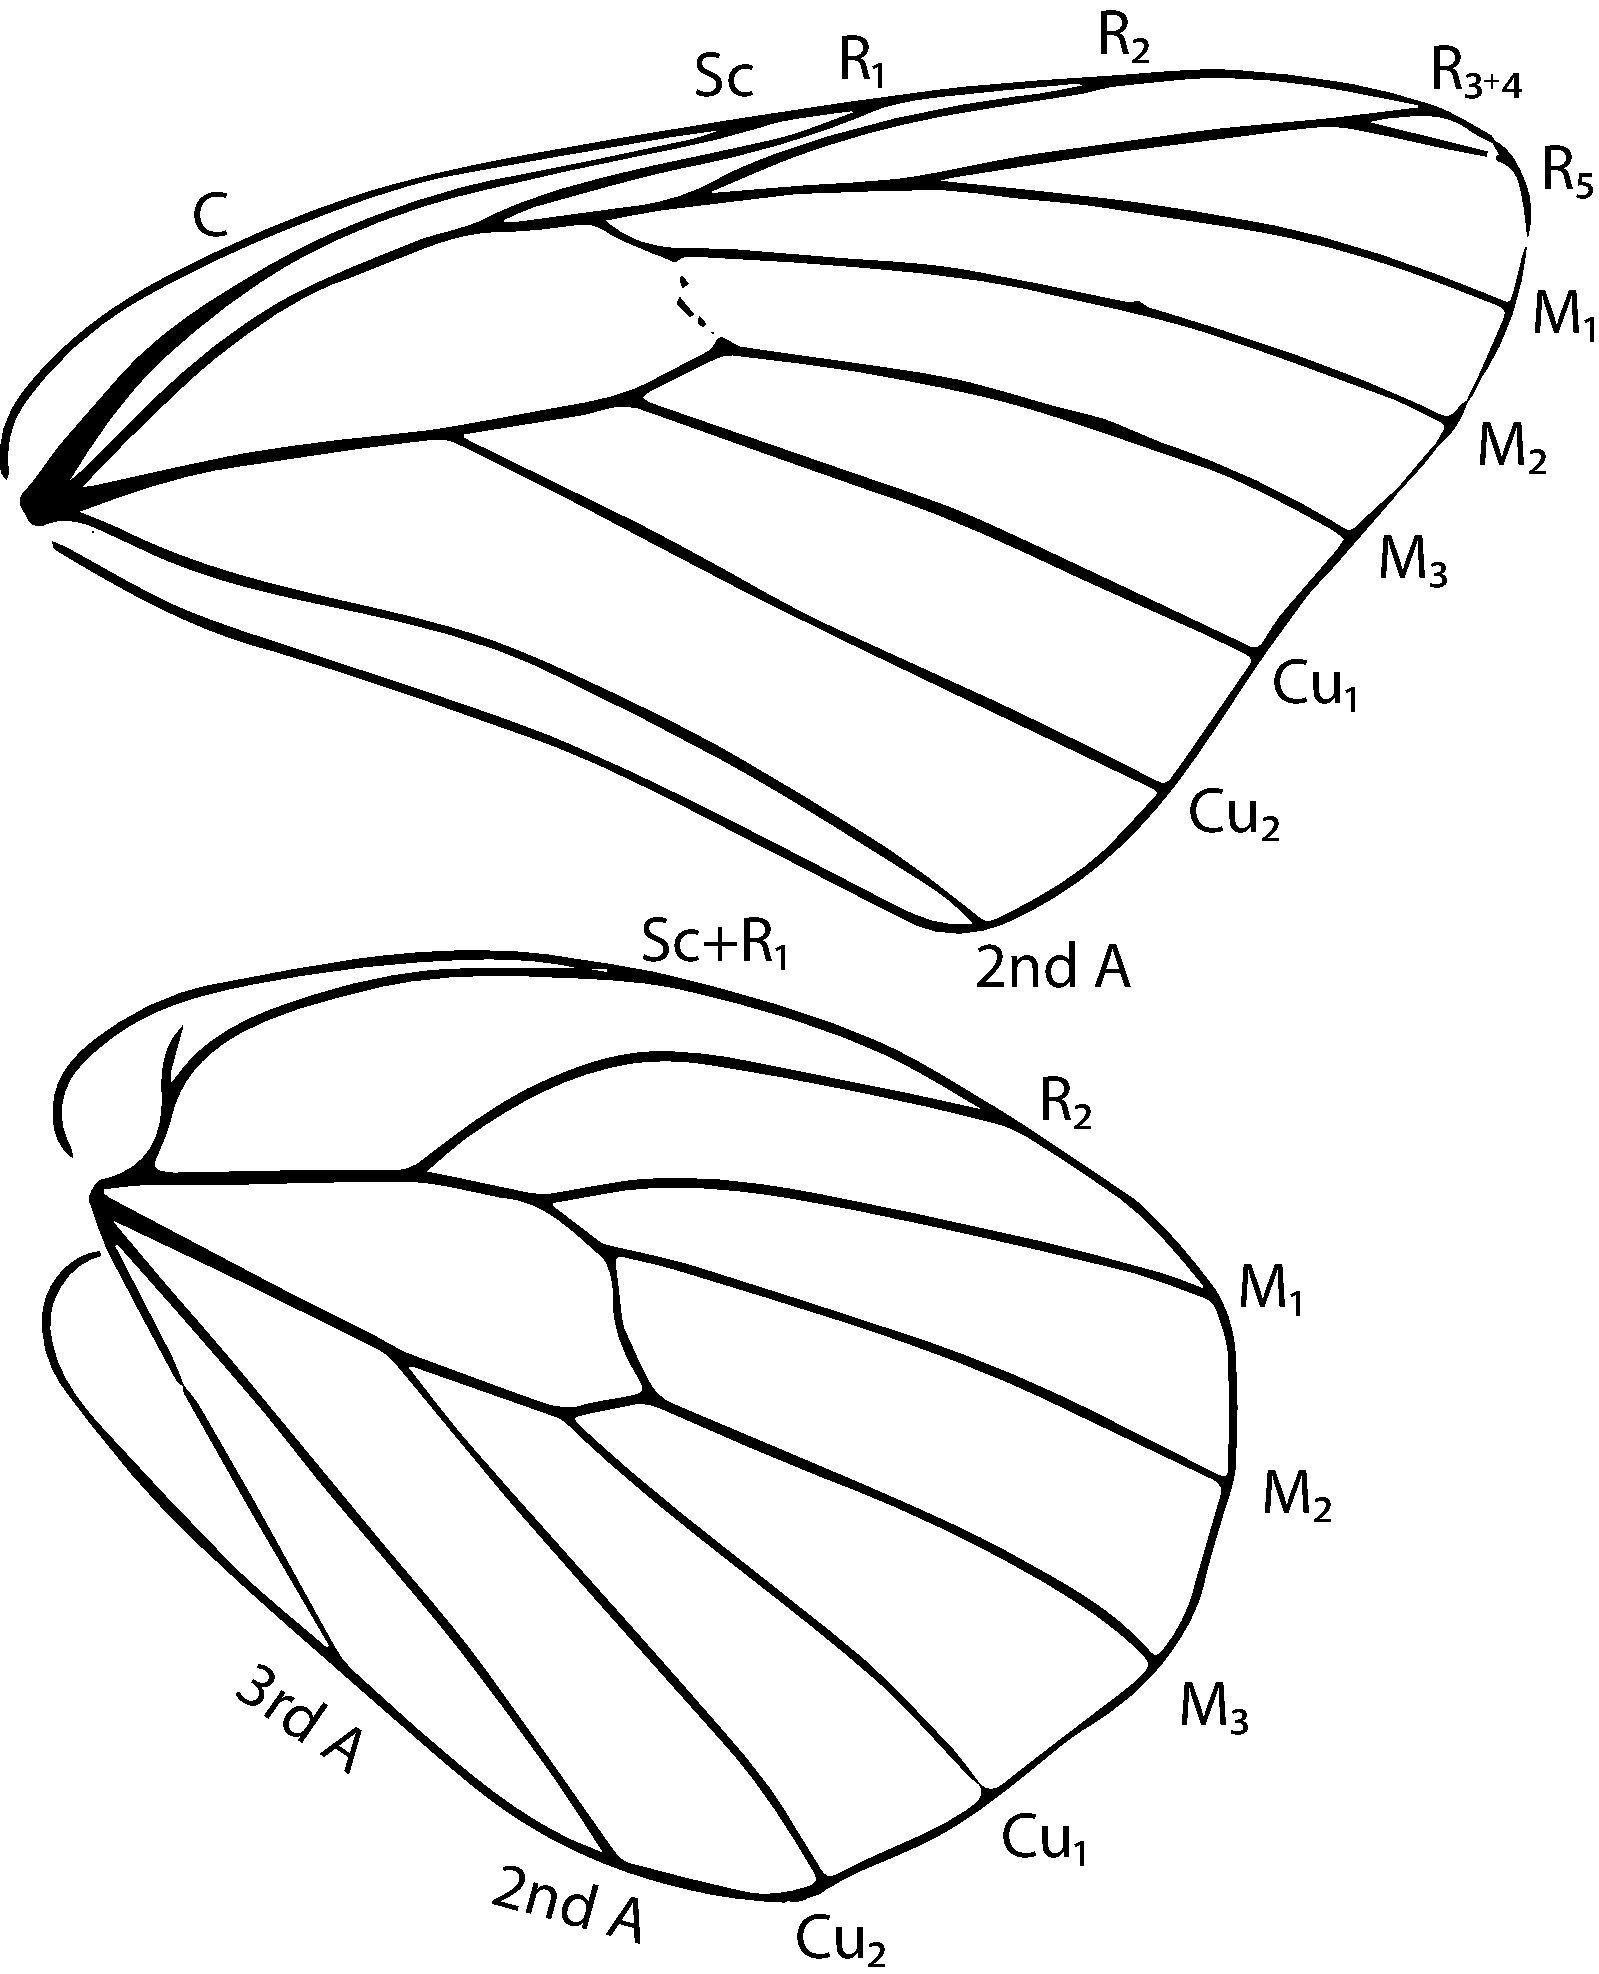
\includegraphics[width=\textwidth]{amphiesmenoptera/PieridWings}
        \caption{}
        \label{fig:pierid1}
    \end{subfigure}
    \hfill
    \begin{subfigure}[ht!]{0.5\textwidth}
        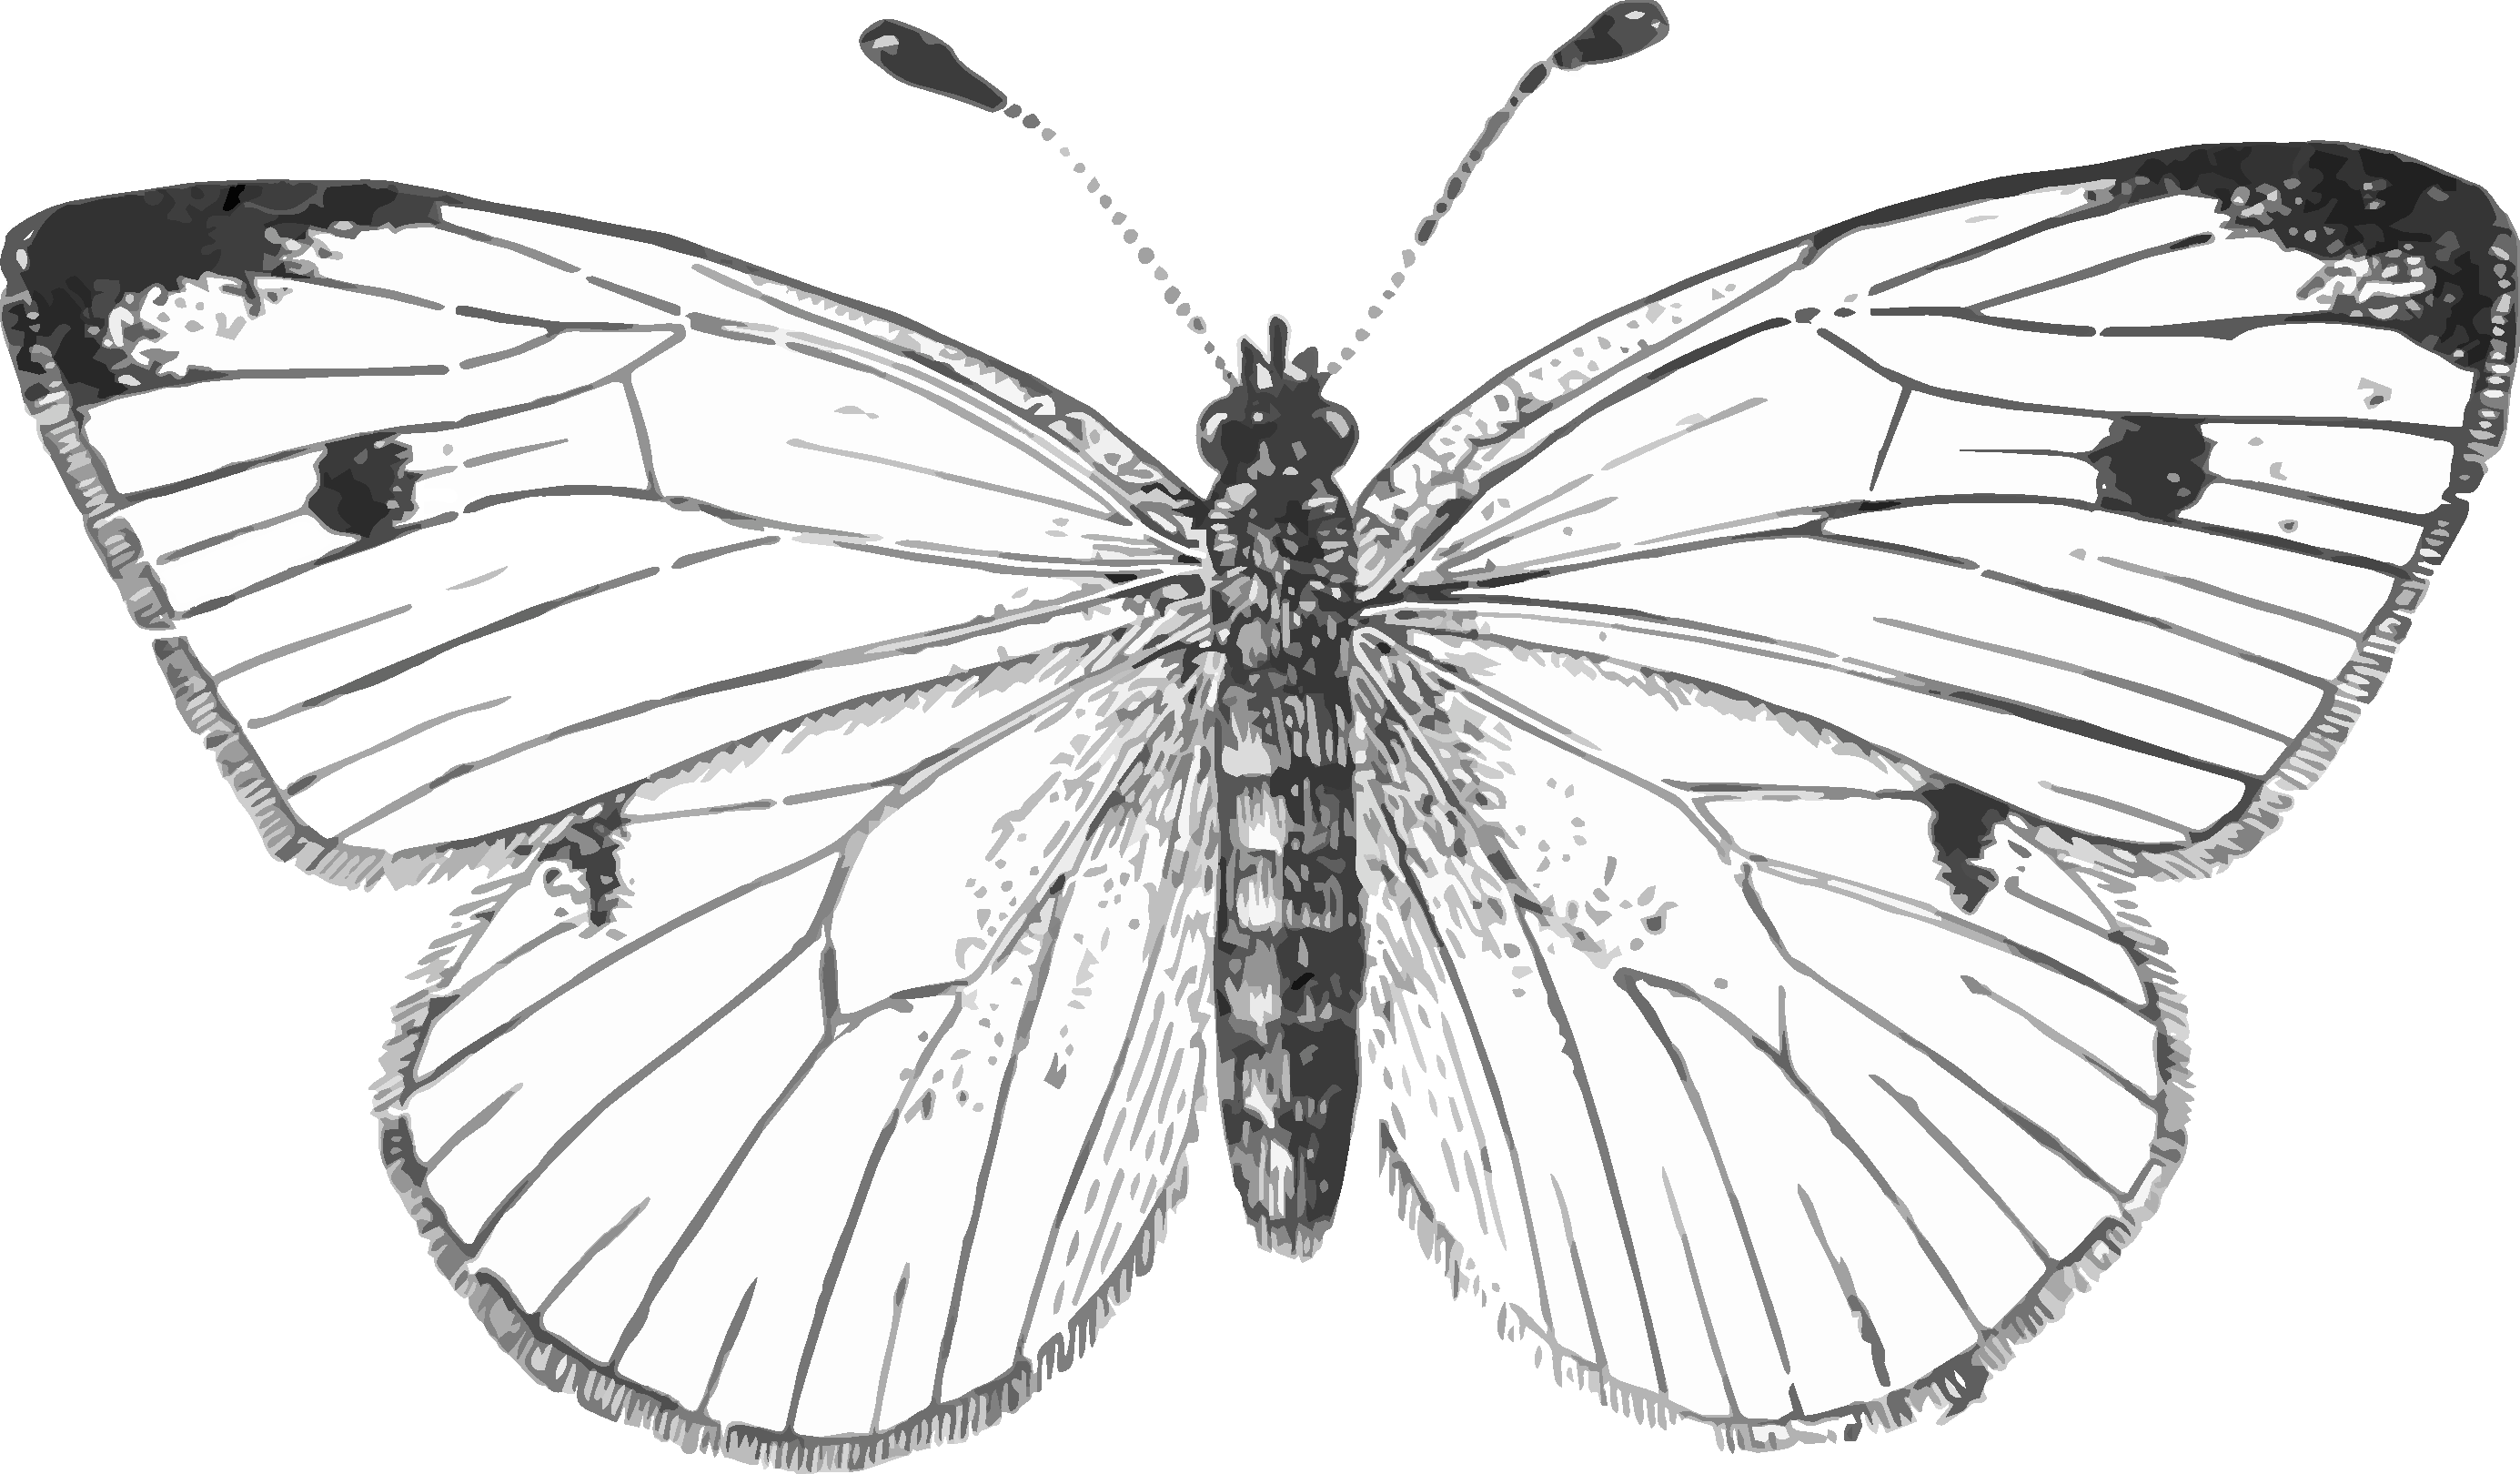
\includegraphics[width=\textwidth]{amphiesmenoptera/pieris}
        \caption{}
        \label{fig:pierid2}
    \end{subfigure}
    \caption{Pieridae. \textbf{(a)} Wings \citep[Fig. 342]{comstock1918wings}; \textbf{(b)} habitus \citep[Modified from Fig. 28 in][]{bhlitem37741}}\label{fig:pierids}
\end{figure}

\subsubsection{Lycaenidae (blues, coppers, hairstreaks)}\index{Lycaenidae}
\noindent{}\textit{Diagnostic characters:} Body small, delicate, and often brightly colored (but usually not white or yellow); antennae usually striped (figure \ref{fig:lycaenid2}); fore wing R 3--4-branched; fore wing M1 very rarely stalked with a branch of R near wing tip; hind wing with 2 anal veins (figure \ref{fig:lycaenid1}), occasionally with very tiny hair-like tail; male fore legs sometimes strongly reduced.\vspace{3mm}

\noindent{}\textit{Natural history:} Second largest group of butterflies, with \textgreater{}5,000 species that tend to be on the small side (wingspan \textless4 cm). Larvae are often closely associated with ants. \vspace{3mm}

\begin{figure}[ht!]
    \centering
    \begin{subfigure}[ht!]{0.27\textwidth}
        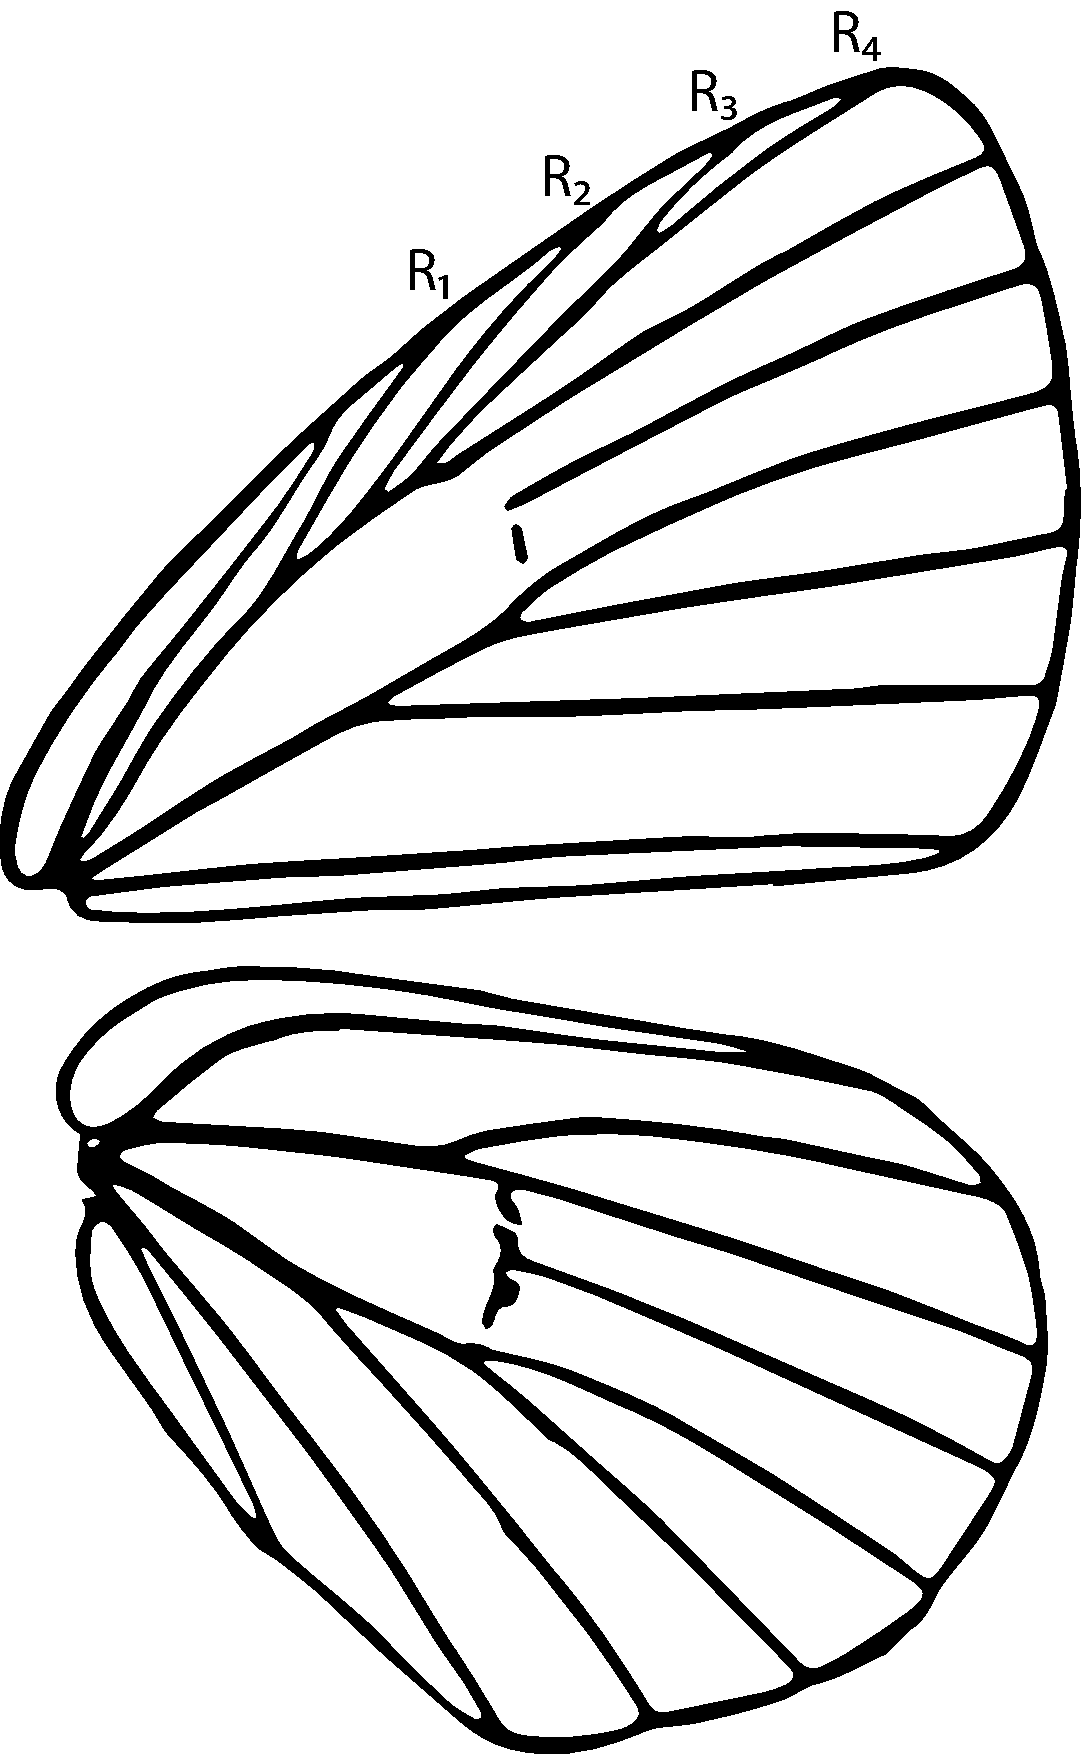
\includegraphics[width=\textwidth]{amphiesmenoptera/LycaenidWings}
        \caption{}
        \label{fig:lycaenid1}
    \end{subfigure}
    \hfill
    \begin{subfigure}[ht!]{0.53\textwidth}
        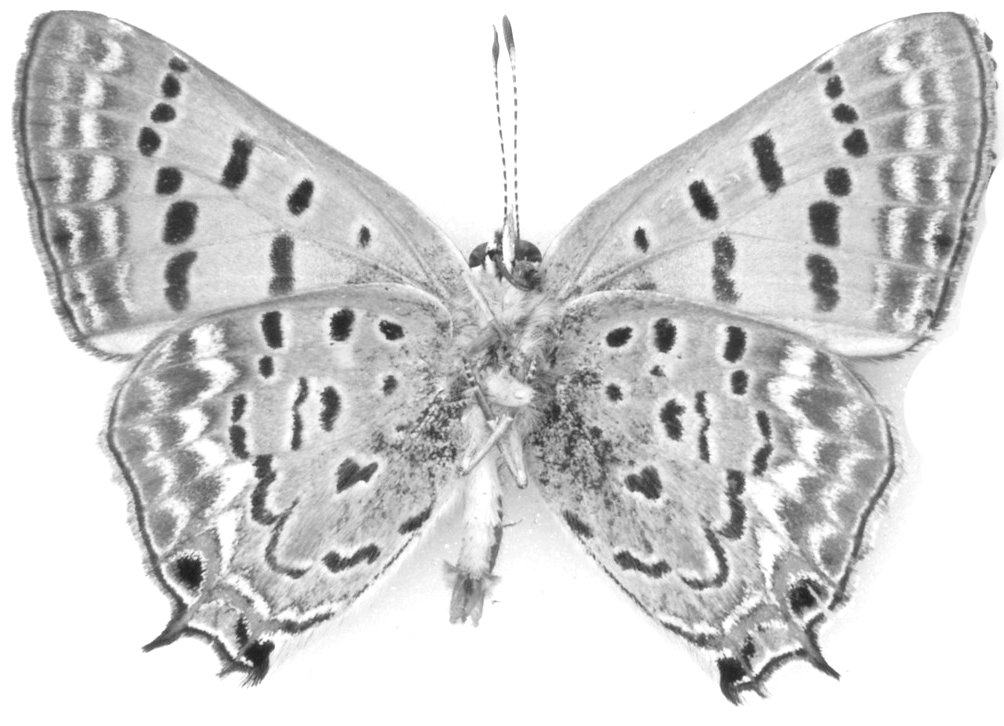
\includegraphics[width=\textwidth]{amphiesmenoptera/lycaenid}
        \caption{}
        \label{fig:lycaenid2}
    \end{subfigure}
    \caption{Lycaenidae. \textbf{(a)} Wings \citep[][Fig. 136]{bhl162310}; \textbf{(b)} ventral habitus Photo (CC0) by Robb Hannawacker \url{https://flic.kr/p/2kBe85b}}\label{fig:lycaenids}
\end{figure}

\FloatBarrier
\paragraph{Macrolepidoptera (excluding Rhopalocera)}\index{Macrolepidoptera} The remaining families are moths that tend to be relatively large and generally share these characters: hind wing with only 1 or 2 anal veins; fore wing with 1 anal vein reaching margin.\vspace{3mm}

\subsubsection{Sphingidae (hawk moths)}\index{Sphingidae}
\noindent{}\textit{Diagnostic characters:} Body robust; head, including eyes, large (figure \ref{fig:sphingid2}); antennae spindle-shaped; ocelli absent; proboscis long, prominent; fore wings narrow, usually much larger than hind wings; hind wing with crossvein midlength in discal cell (arrow in figure \ref{fig:sphingid1}); abdomen often pointed.\vspace{3mm}

\noindent{}\textit{Natural history:} Larvae usually have dorsal, horn-like evagination on their posterior end, sometimes reduced or even absent. Adults are strong fliers. There are more than 1,400 described species.\vspace{3mm}

\begin{figure}[ht!]
    \centering
    \begin{subfigure}[ht!]{0.35\textwidth}
        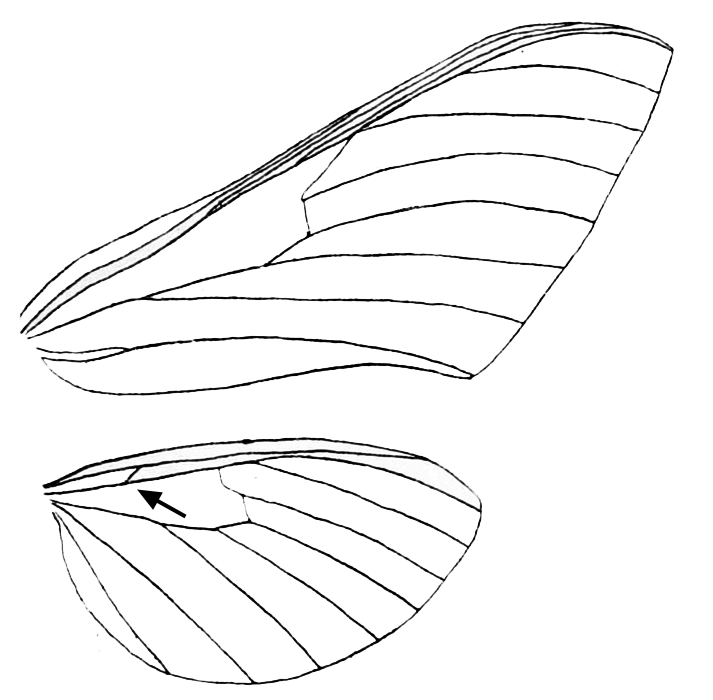
\includegraphics[width=\textwidth]{amphiesmenoptera/SphingidWings}
        \caption{}
        \label{fig:sphingid1}
    \end{subfigure}
    \hfill
    \begin{subfigure}[ht!]{0.6\textwidth}
        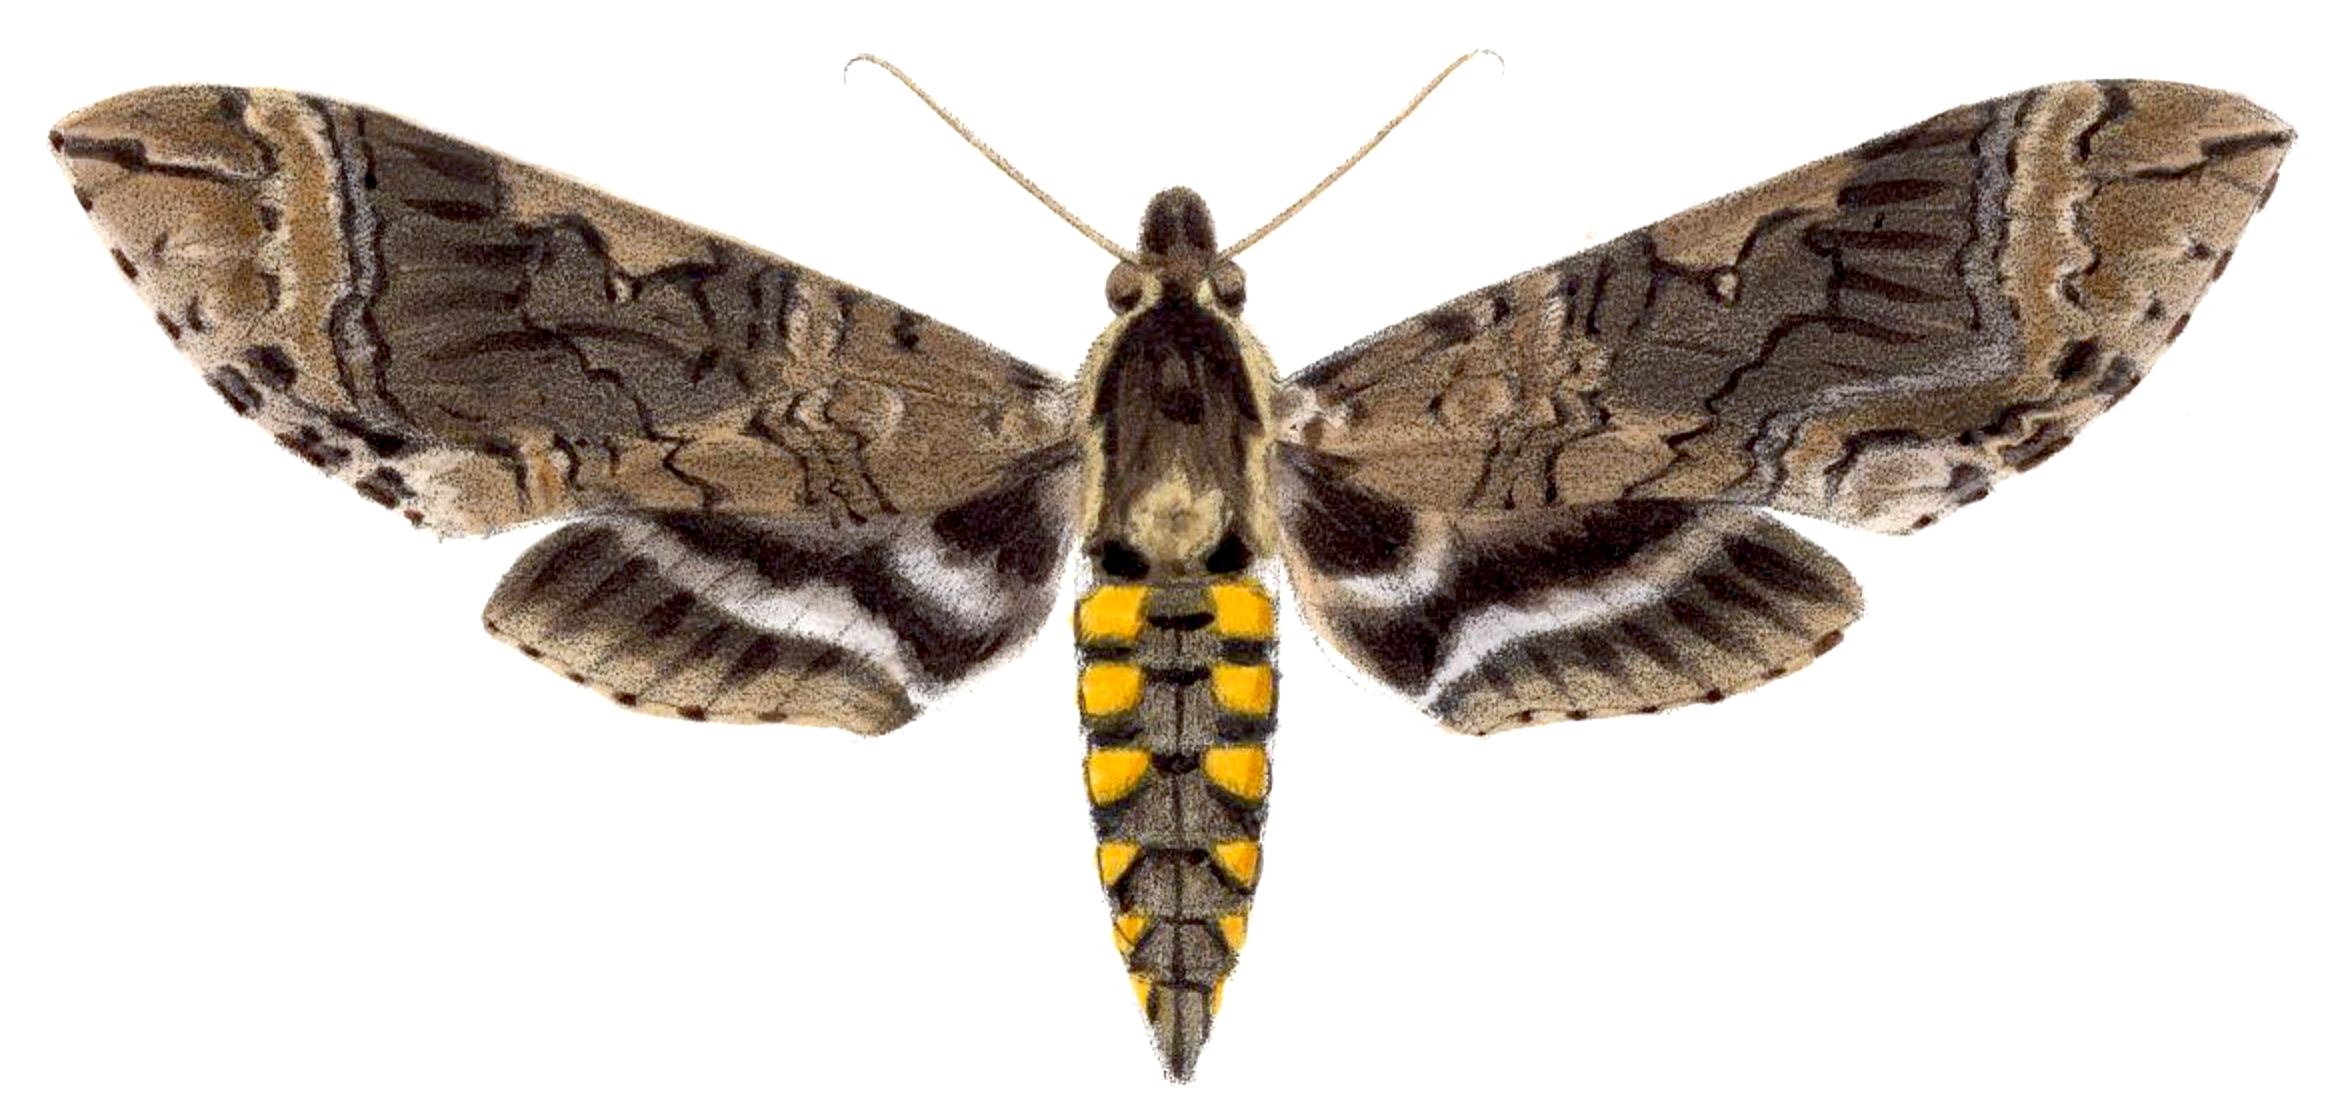
\includegraphics[width=\textwidth]{amphiesmenoptera/SphingidHabitus}
        \caption{}
        \label{fig:sphingid2}
    \end{subfigure}
    \caption{Sphingidae. \textbf{(a)} Wings \citep[][Plate XIII, Fig. 3]{bhl38041}; \textbf{(b)} habitus \citep[][Plate 67, Fig. 4]{druce1900biologia}}\label{fig:sphingids}
\end{figure}

\subsubsection{Saturniidae (giant silk moths)}\index{Saturniidae}
\noindent{}\textit{Diagnostic characters:} Antennae often bipectinate (figure \ref{fig:saturniid2}); proboscis reduced or absent; wings usually with translucent patches (``eye spots''; see figure \ref{fig:saturniid2}); fore wing M2 arising closer to M1 than M3 (figure \ref{fig:saturniid1}); no basal areole in hind wing; hind wing Sc and Rs not fused; frenulum absent (wing coupling amplexiform); frenulum absent; medium-sized to large (wingspan up to 15 cm), with broad wings and short, thick bodies.\vspace{3mm}

\noindent{}\textit{Natural history:} Caterpillars diversely phytophagous, generally among the largest lepidopteran larvae. Most species pupate inside a silken cocoon. There are more than 2,300 described species.

\begin{figure}[ht!]
    \centering
    \begin{subfigure}[ht!]{0.31\textwidth}
        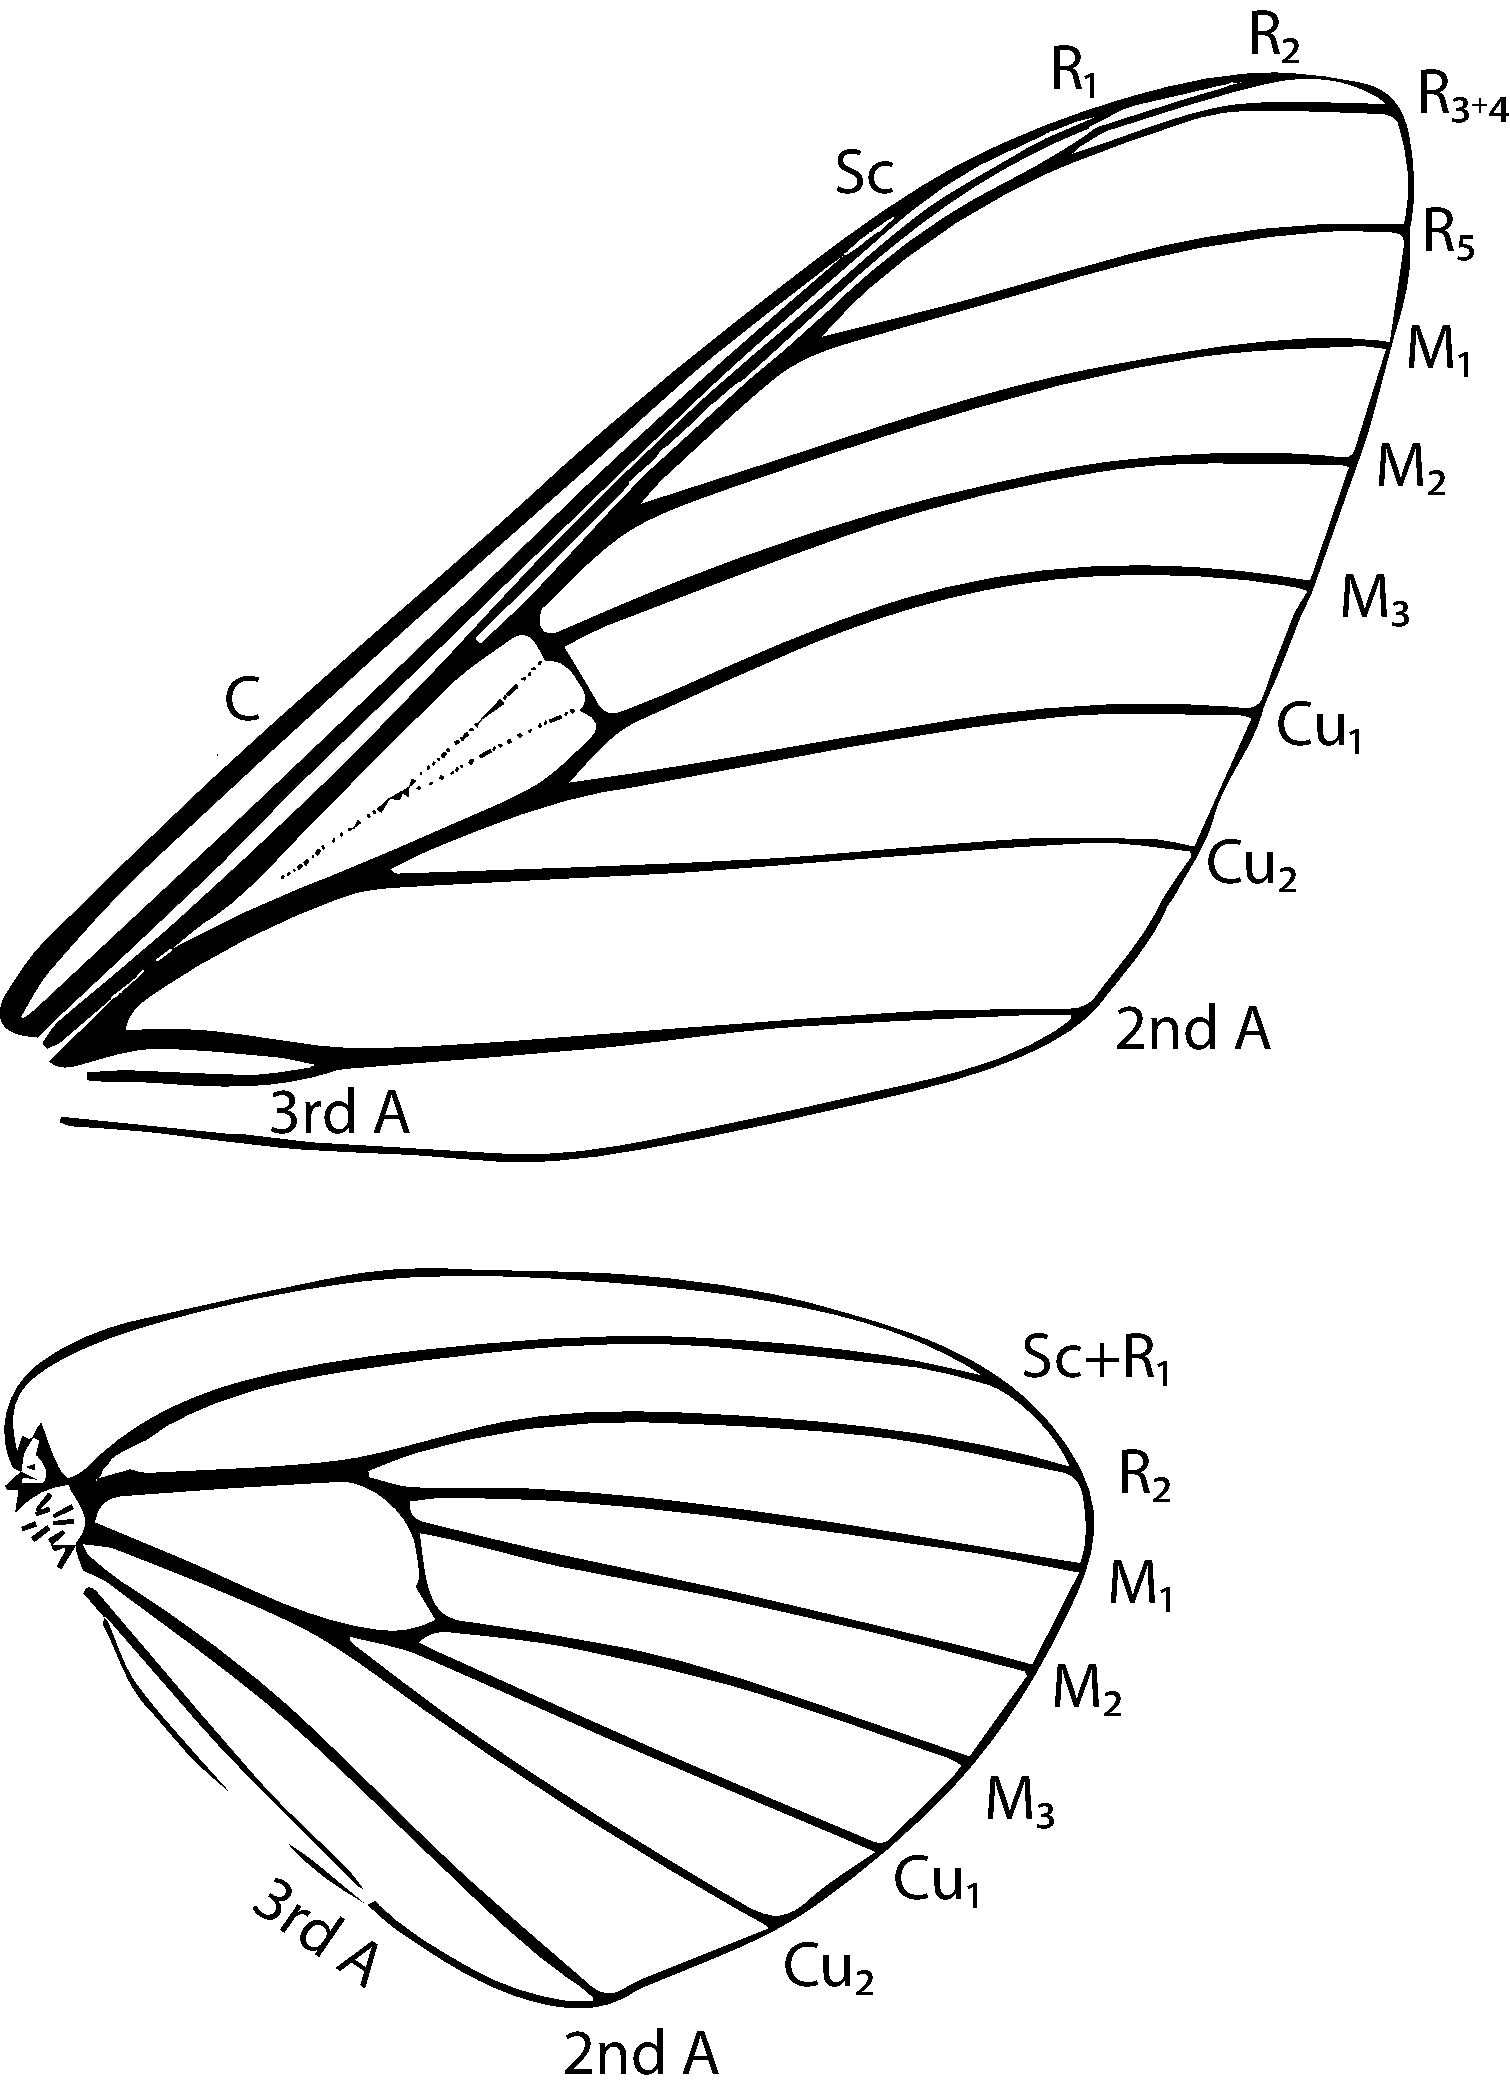
\includegraphics[width=\textwidth]{amphiesmenoptera/SaturniidWings}
        \caption{}
        \label{fig:saturniid1}
    \end{subfigure}
    \hfill
    \begin{subfigure}[ht!]{0.6\textwidth}
        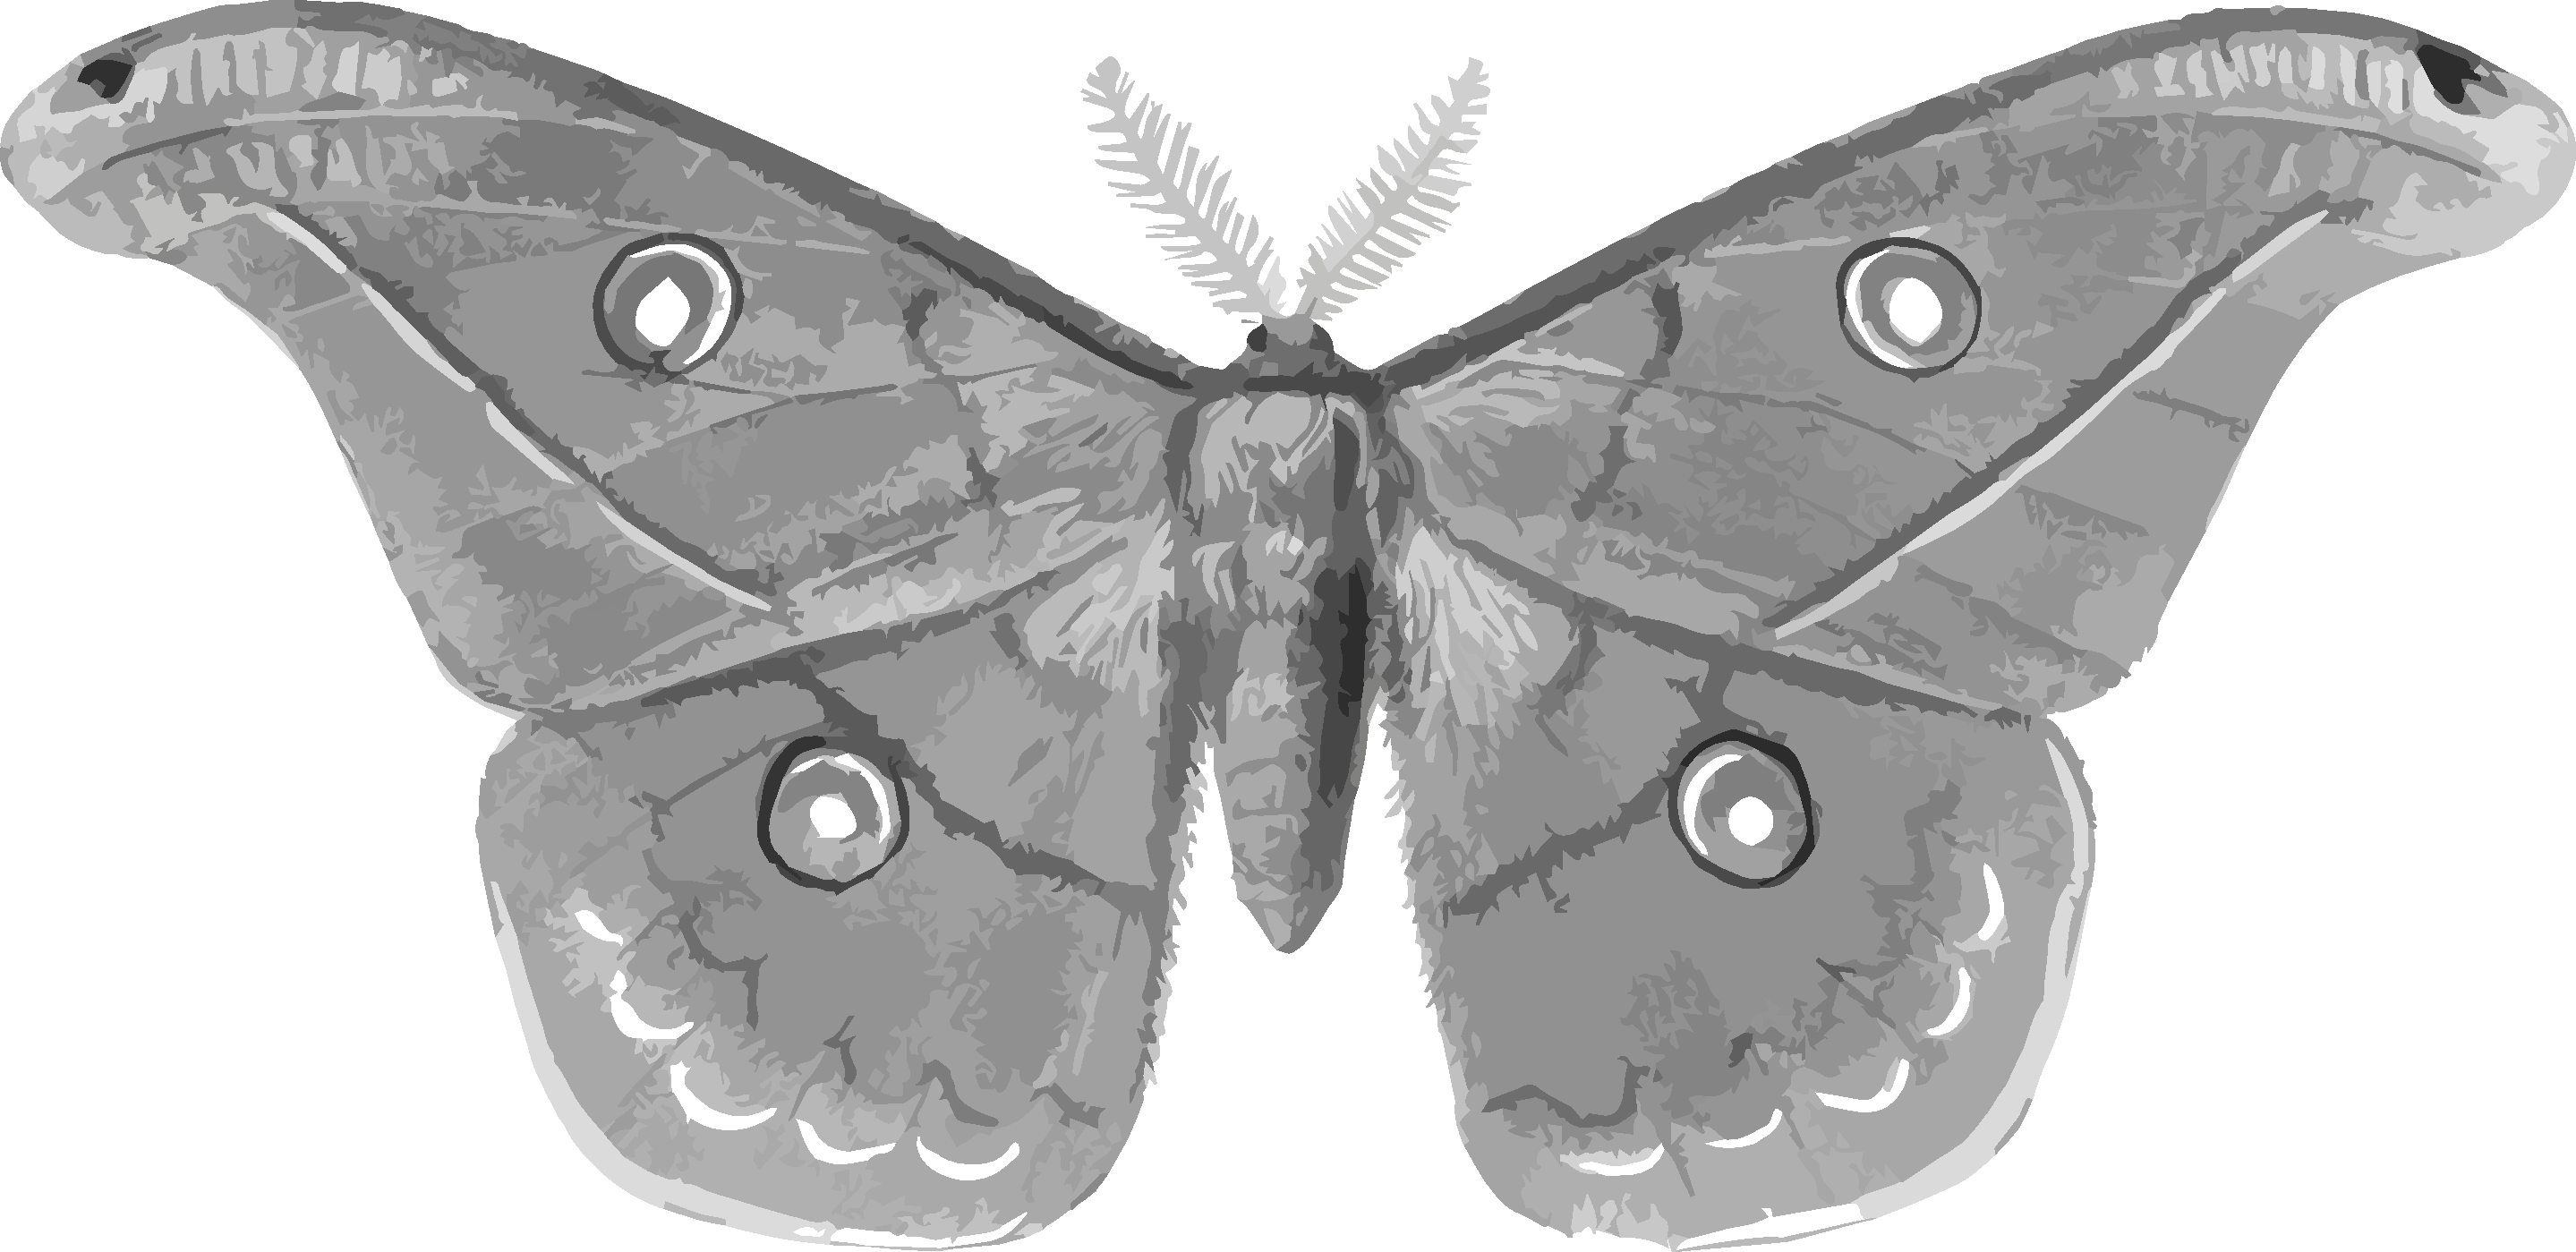
\includegraphics[width=\textwidth]{amphiesmenoptera/SaturniidHabitus}
        \caption{}
        \label{fig:saturniid2}
    \end{subfigure}
    \caption{Saturniidae. \textbf{(a)} Wings \citep[Fig. 345]{comstock1918wings}; \textbf{(b)} habitus \citep[][Plate 19, Fig. 1]{druce1900biologia}}\label{fig:saturniids}
\end{figure}

\subsubsection{Lasiocampidae (tent caterpillars, lappet moths, eggars)}\index{Lasiocampidae}
\noindent{}\textit{Diagnostic characters:} Antennae bipectinate; proboscis vestigial or absent; fore wing Cu2 arising near wing base; basal areole present in hind wing; frenulum absent, humeral area of hind wing greatly expanded (figure \ref{fig:lasiocampid1}); fore wing M2 arising closer to M3 than M1; relatively fat-bodied and hairy moths (figure \ref{fig:lasiocampid2}).\vspace{3mm}

\noindent{}\textit{Natural history:} Caterpillars diversely phytophagous but mostly on leaves of trees and shrubs. caterpillars setose, often with flattened evaginations (flaps or ``lappets'') near the prolegs. Some species live communally in tents during the larval stages. About 2,000 species have been described worldwide.

\begin{figure}[ht!]
    \centering
    \begin{subfigure}[ht!]{0.3\textwidth}
        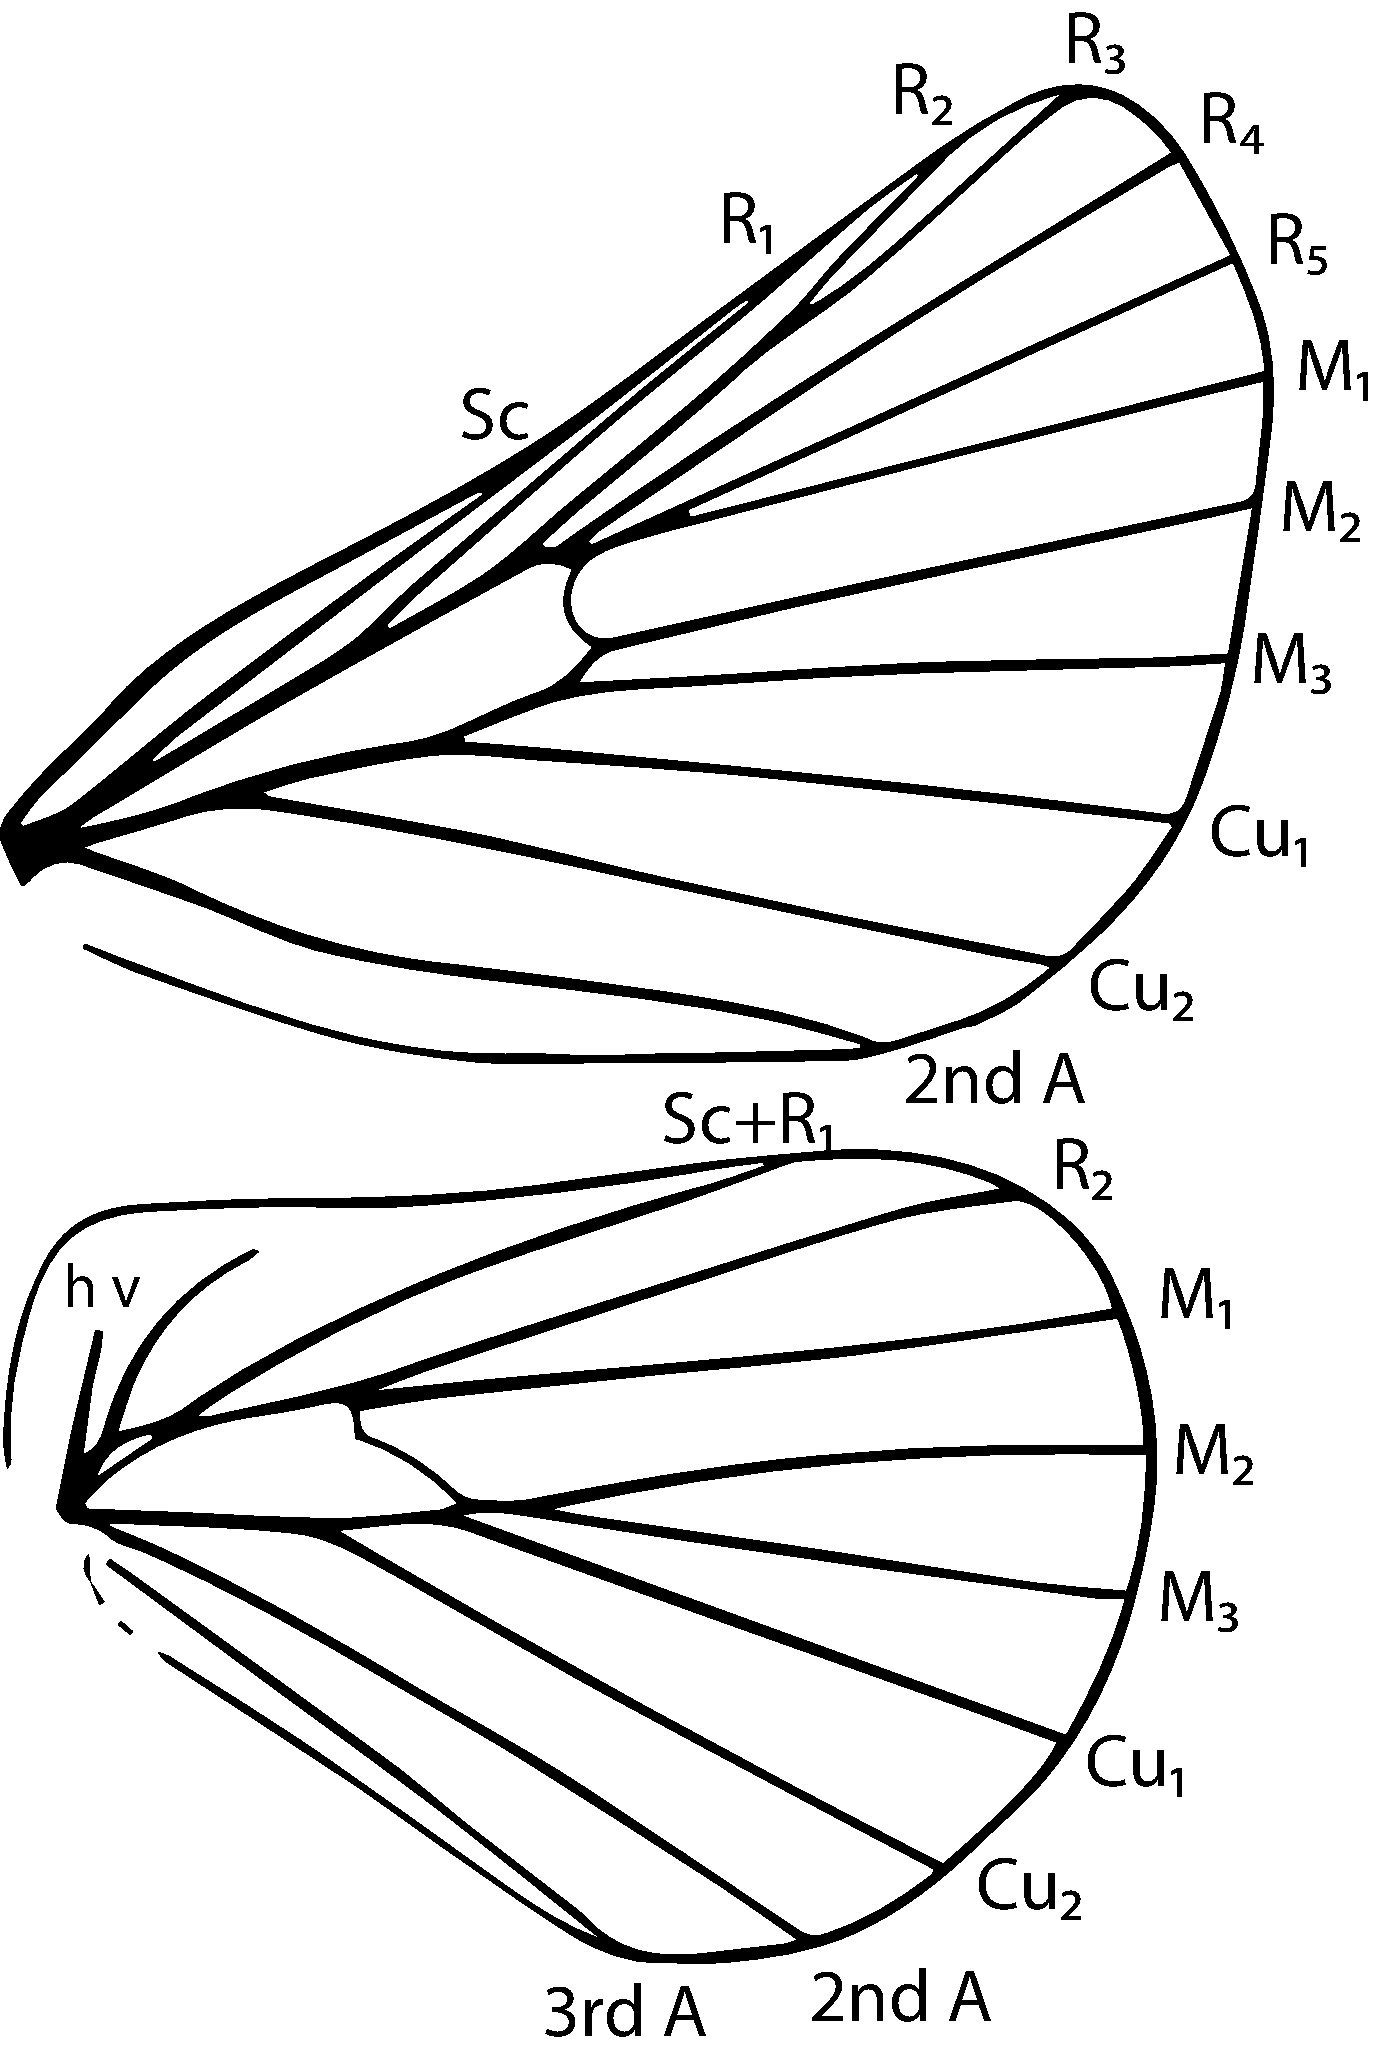
\includegraphics[width=\textwidth]{amphiesmenoptera/LasiocampidWings}
        \caption{}
        \label{fig:lasiocampid1}
    \end{subfigure}
    \hfill
    \begin{subfigure}[ht!]{0.5\textwidth}
        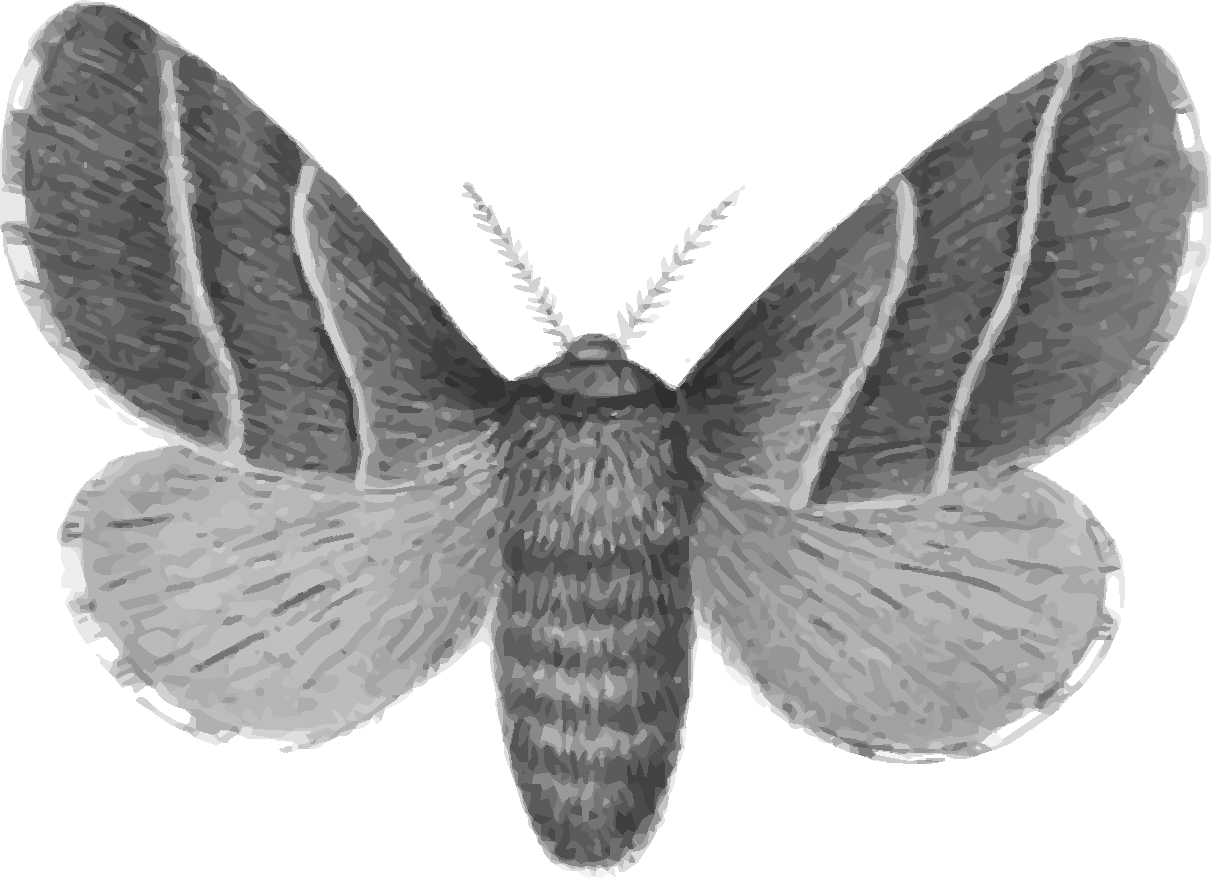
\includegraphics[width=\textwidth]{amphiesmenoptera/lasiocampidHabitus}
        \caption{}
        \label{fig:lasiocampid2}
    \end{subfigure}
    \caption{Lasiocampidae. \textbf{(a)} Wings \citep[Fig. 69]{comstock1918wings}; \textbf{(b)} habitus \citep[Plate 39, Fig. 9]{bhlitem92348}}\label{fig:lasiocampids}
\end{figure}

\subsubsection{Notodontidae (prominents)}\index{Notodontidae}%teach as Noctuoidea?
\noindent{}\textit{Diagnostic characters:} Antennae usually bipectinate; tympanum on metathorax pointing ventrally; tympanal hood absent; no basal areole in hind wing; Sc and Rs in hind wing parallel, not usually fused; fore wing M2 arising in midway between M1 and M3 (key character to separate from Noctuidae and Erebidae; see figure \ref{fig:notodontid1}); fore wing usually conspicuously longer than hind wing; body relatively stout, usually drab-colored (figure \ref{fig:notodontid2}).\vspace{3mm}

\noindent{}\textit{Natural history:} There are almost 4,000 species of prominents worldwide. Larvae typically feed on trees and have a distinctive habitus. Adults do not feed.\vspace{3mm}

\begin{figure}[ht!]
    \centering
    \begin{subfigure}[ht!]{0.32\textwidth}
        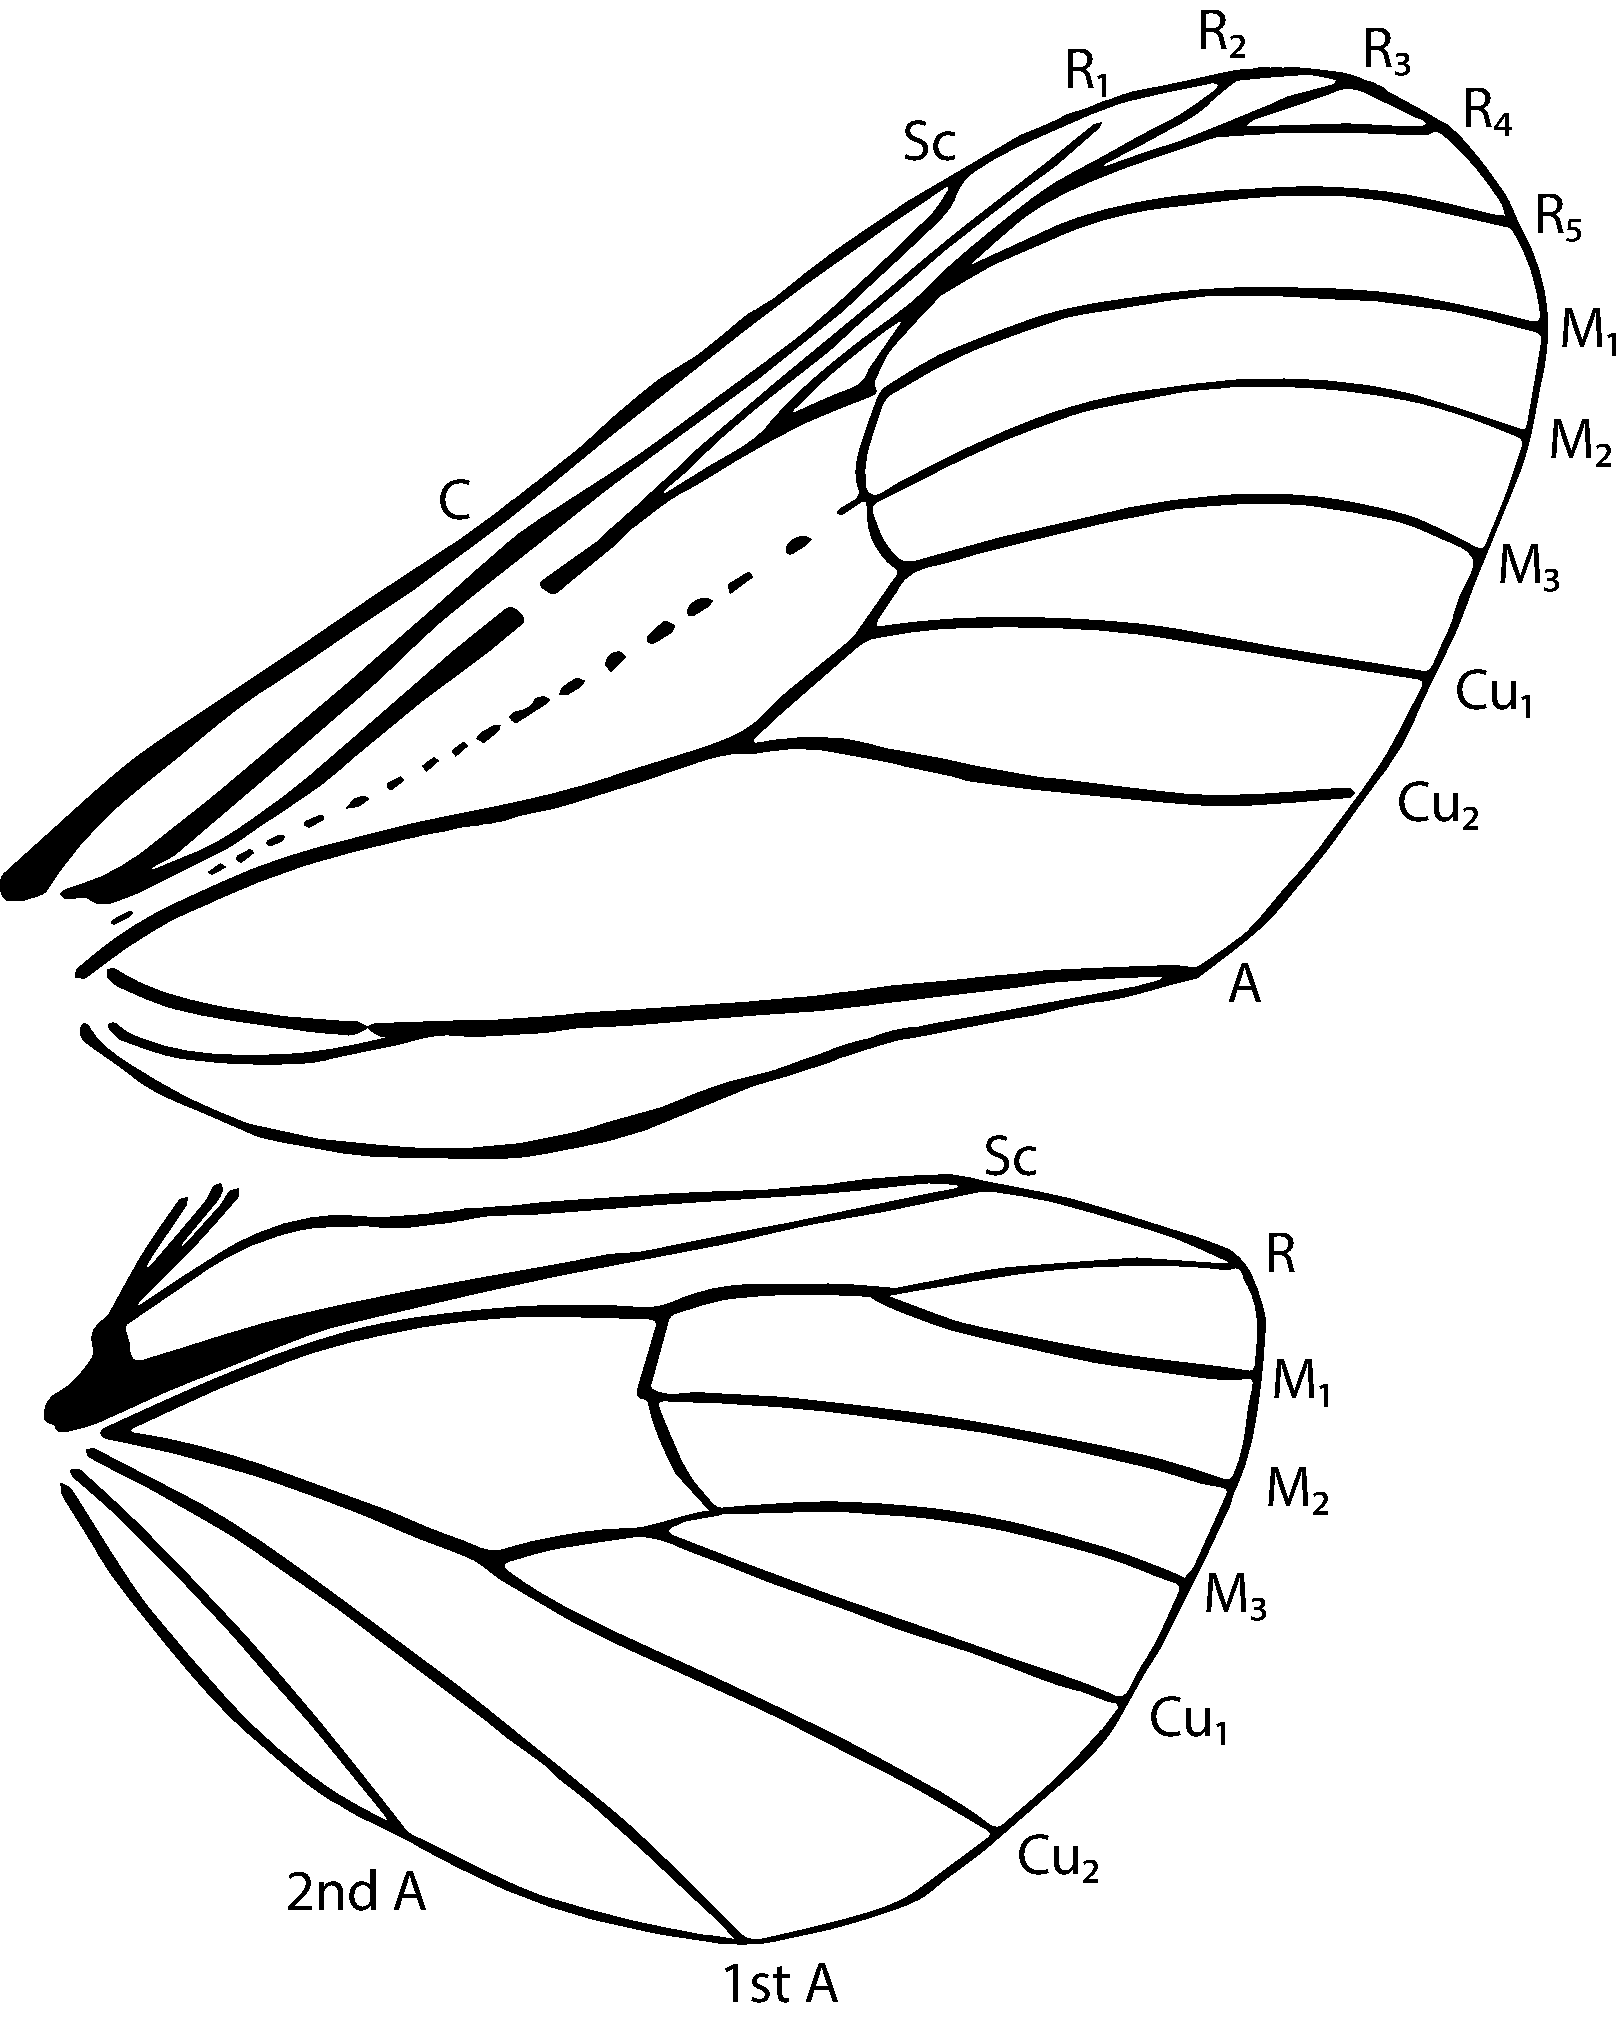
\includegraphics[width=\textwidth]{amphiesmenoptera/NotodontidWings}
        \caption{}
        \label{fig:notodontid1}
    \end{subfigure}
    \hfill 
    \begin{subfigure}[ht!]{0.5\textwidth}
        \includegraphics[width=\textwidth]{amphiesmenoptera/notodontidHabitus}
        \caption{}
        \label{fig:notodontid2}
    \end{subfigure}
    \caption{Notodontidae. \textbf{(a)} Wings \citep[][Fig. 443]{bhlitem16791elementary}; \textbf{(b)} habitus (redrawn from photo (CC BY-SA 3.0 unported) by Megan McCarty)} \label{fig:notodontids}
\end{figure}

\begin{theo}
{}How well is the ethanol on the wing trick working for you? Can you see the venation?
\end{theo} 

\subsubsection{Noctuidae (owlet moths)}\index{Noctuidae}
\noindent{}\textit{Diagnostic characters:} Antennae usually simple, occasionally bipectinate, sometimes swol-len apically; labial palps usually long, upturned; ocelli sometimes present, medium-sized to large; fore wings usually cryptic, sometimes with eye-like spots (figure \ref{fig:noctuid1}); hind wing cubital vein branches into 2 or 3 veins (hind wing trifine or bifine; see figure \ref{fig:noctuid1}); tympanum on metathorax pointing posteriorly or outwards; tympanal hood located posterior to spiracle; body color usually dominated by browns.\vspace{3mm}

\noindent{}\textit{Natural history:} Hugely diverse taxon, with tens of thousands of species; its taxonomic limits remain unsettled. Their natural history is difficult to generalize, but these moths are typically night-fliers. Larvae are diversely herbivorous and include many important pest species.

\begin{figure}[ht!]
    \centering
    \begin{subfigure}[ht!]{0.37\textwidth}
        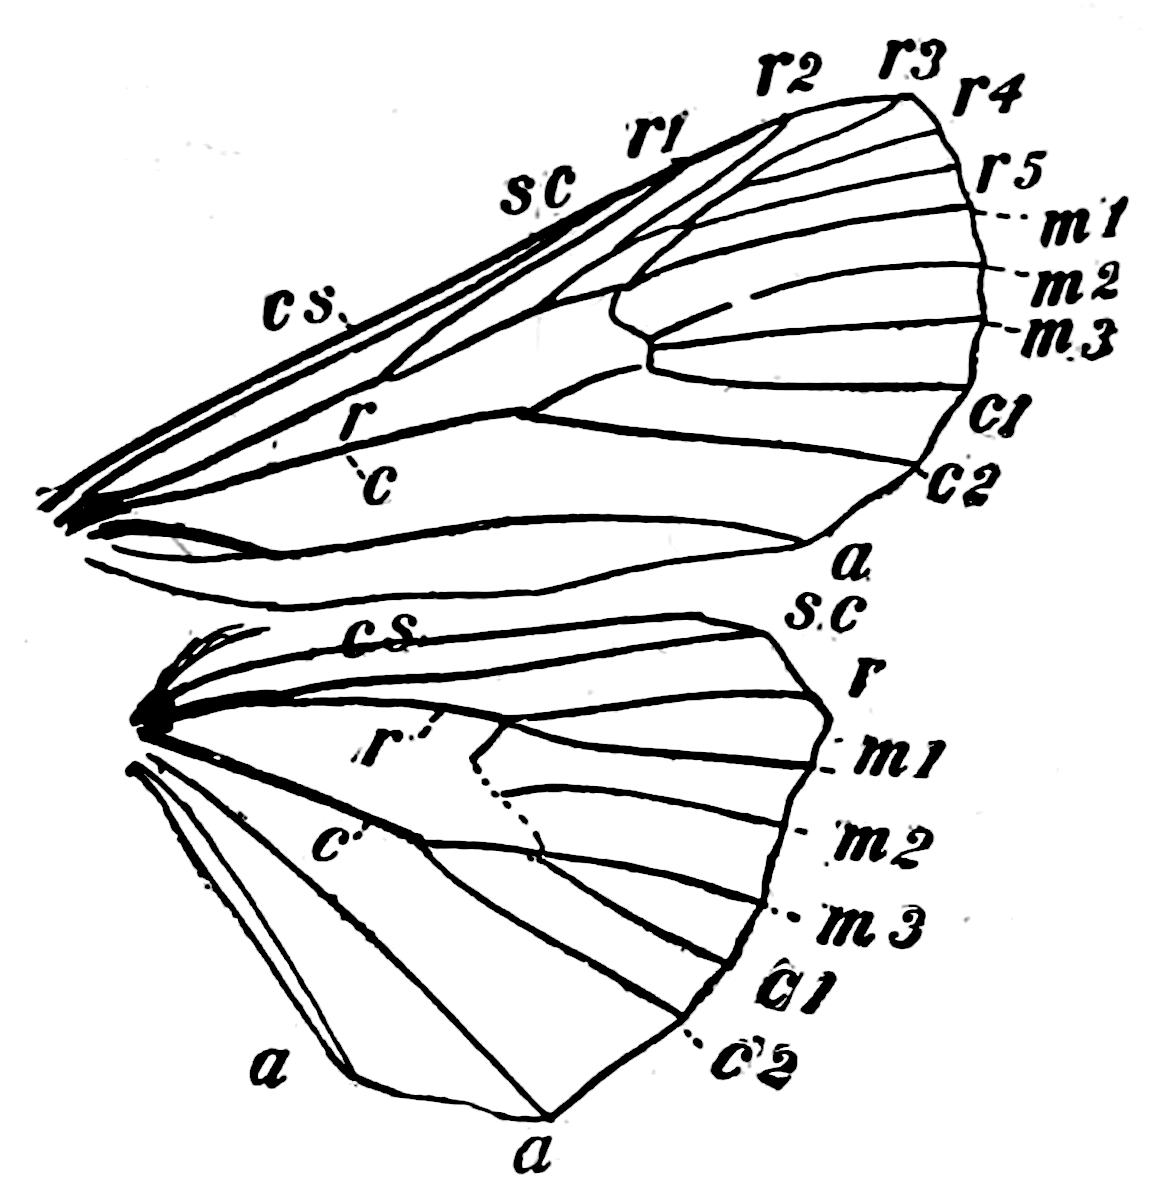
\includegraphics[width=\textwidth]{amphiesmenoptera/NoctuidWings}
        \caption{}
        \label{fig:noctuid1}
    \end{subfigure}
    \qquad
    \begin{subfigure}[ht!]{0.5\textwidth}
        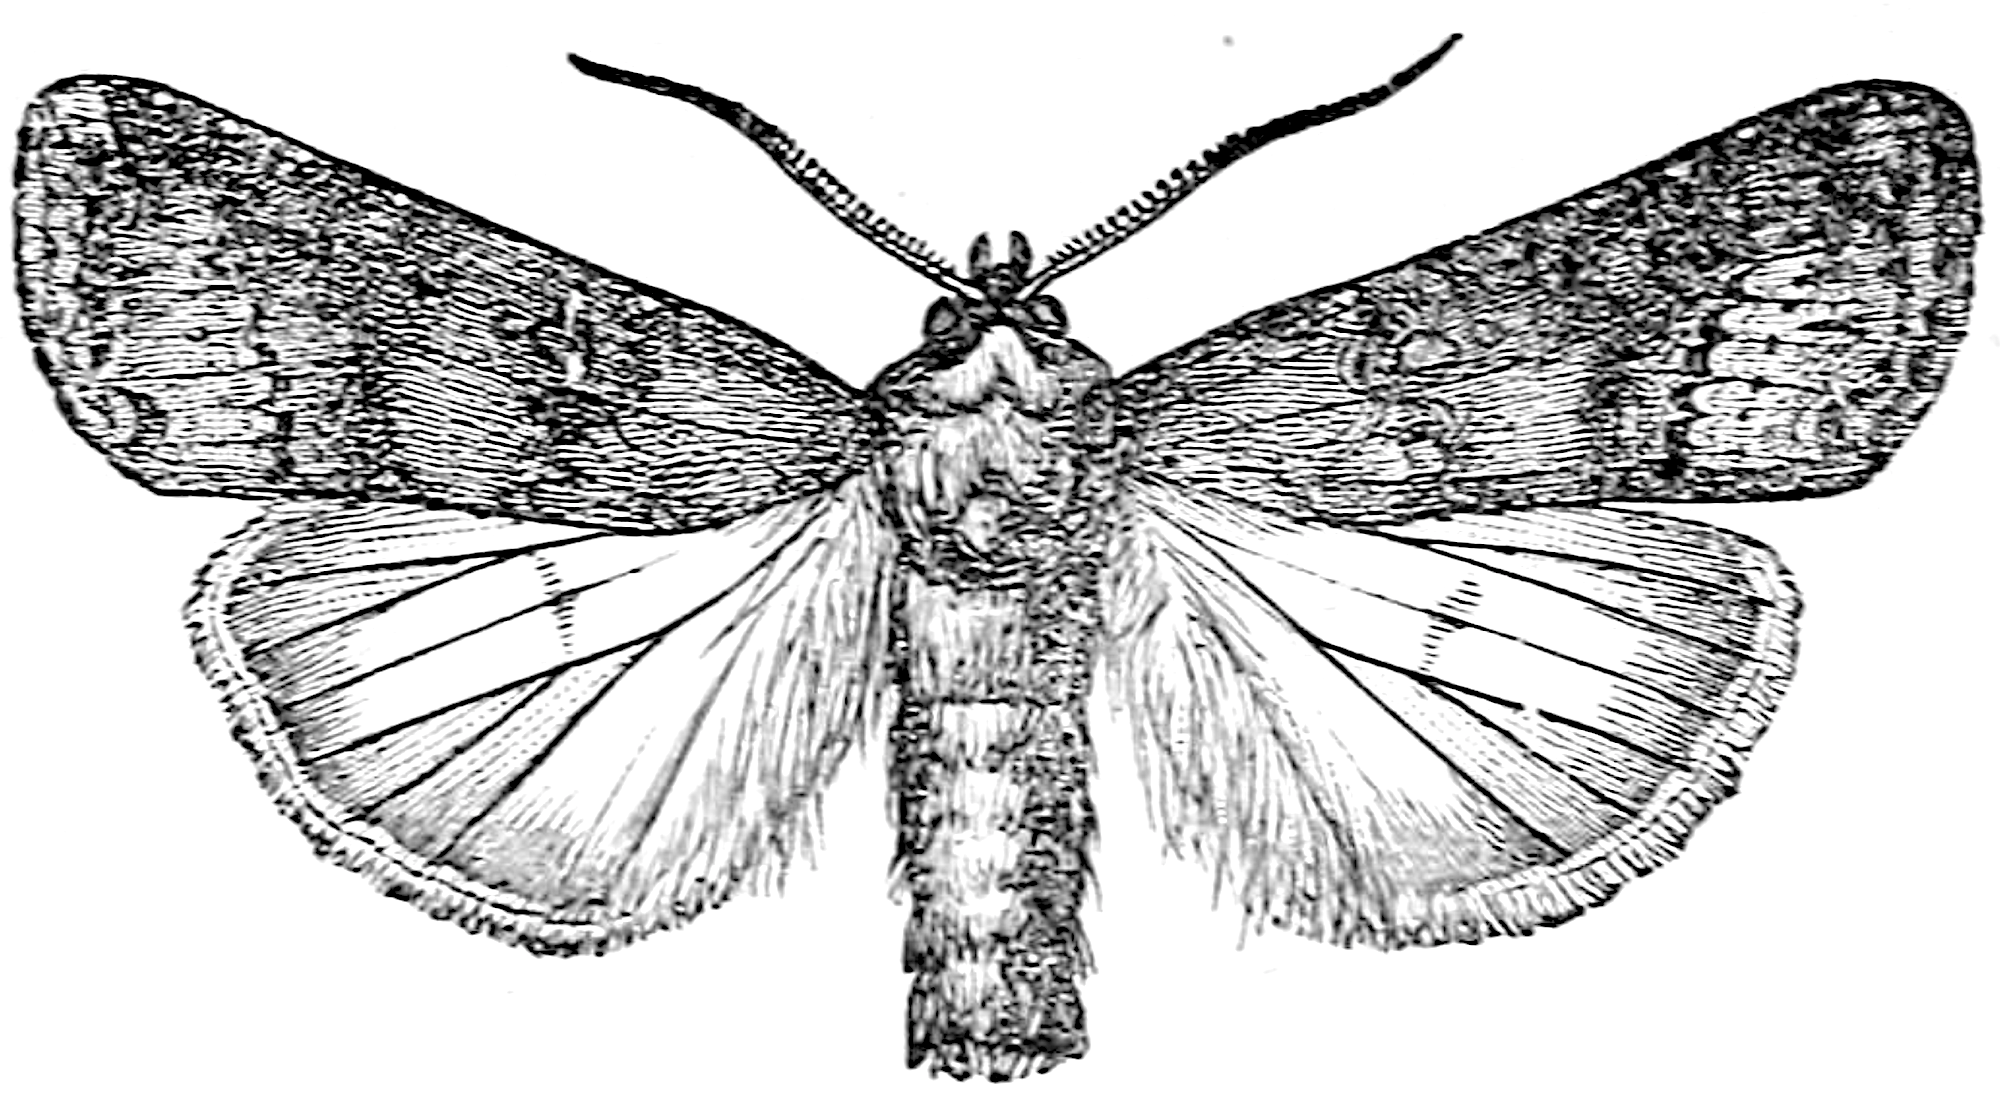
\includegraphics[width=\textwidth]{amphiesmenoptera/noctuidHab}
        \caption{}
        \label{fig:noctuid2}
    \end{subfigure}
    \caption{Noctuidae. \textbf{(a)} Wings \citep[][Fig. 445]{bhlitem16791elementary}; \textbf{(b)} habitus \citep[Modified from Fig. 14 in][]{bhlitem128144}}\label{fig:noctuids}
\end{figure}

\subsubsection{Erebidae (includes Lymantriidae, Arctiidae, and several lineages that used to be in Noctuidae)}\index{Erebidae}
\noindent{}\textit{Diagnostic characters:} Similar to Noctuidae but hind wing cubital vein branches into 4 veins: CU2, CU1, M3, M2 (\textit{i.e.}, hind wing quadrifine; see figure \ref{fig:erebid1}).\vspace{3mm}

\noindent{}\textit{Natural history:} Like Noctuidae, this is a hugely diverse taxon, with tens of thousands of species. Their natural history is difficult to generalize, but these moths are typically night-fliers. Larvae are diversely herbivorous and include many important pest species.\vspace{3mm}

\begin{figure}[ht!]
    \centering
    \begin{subfigure}[ht!]{0.36\textwidth}
        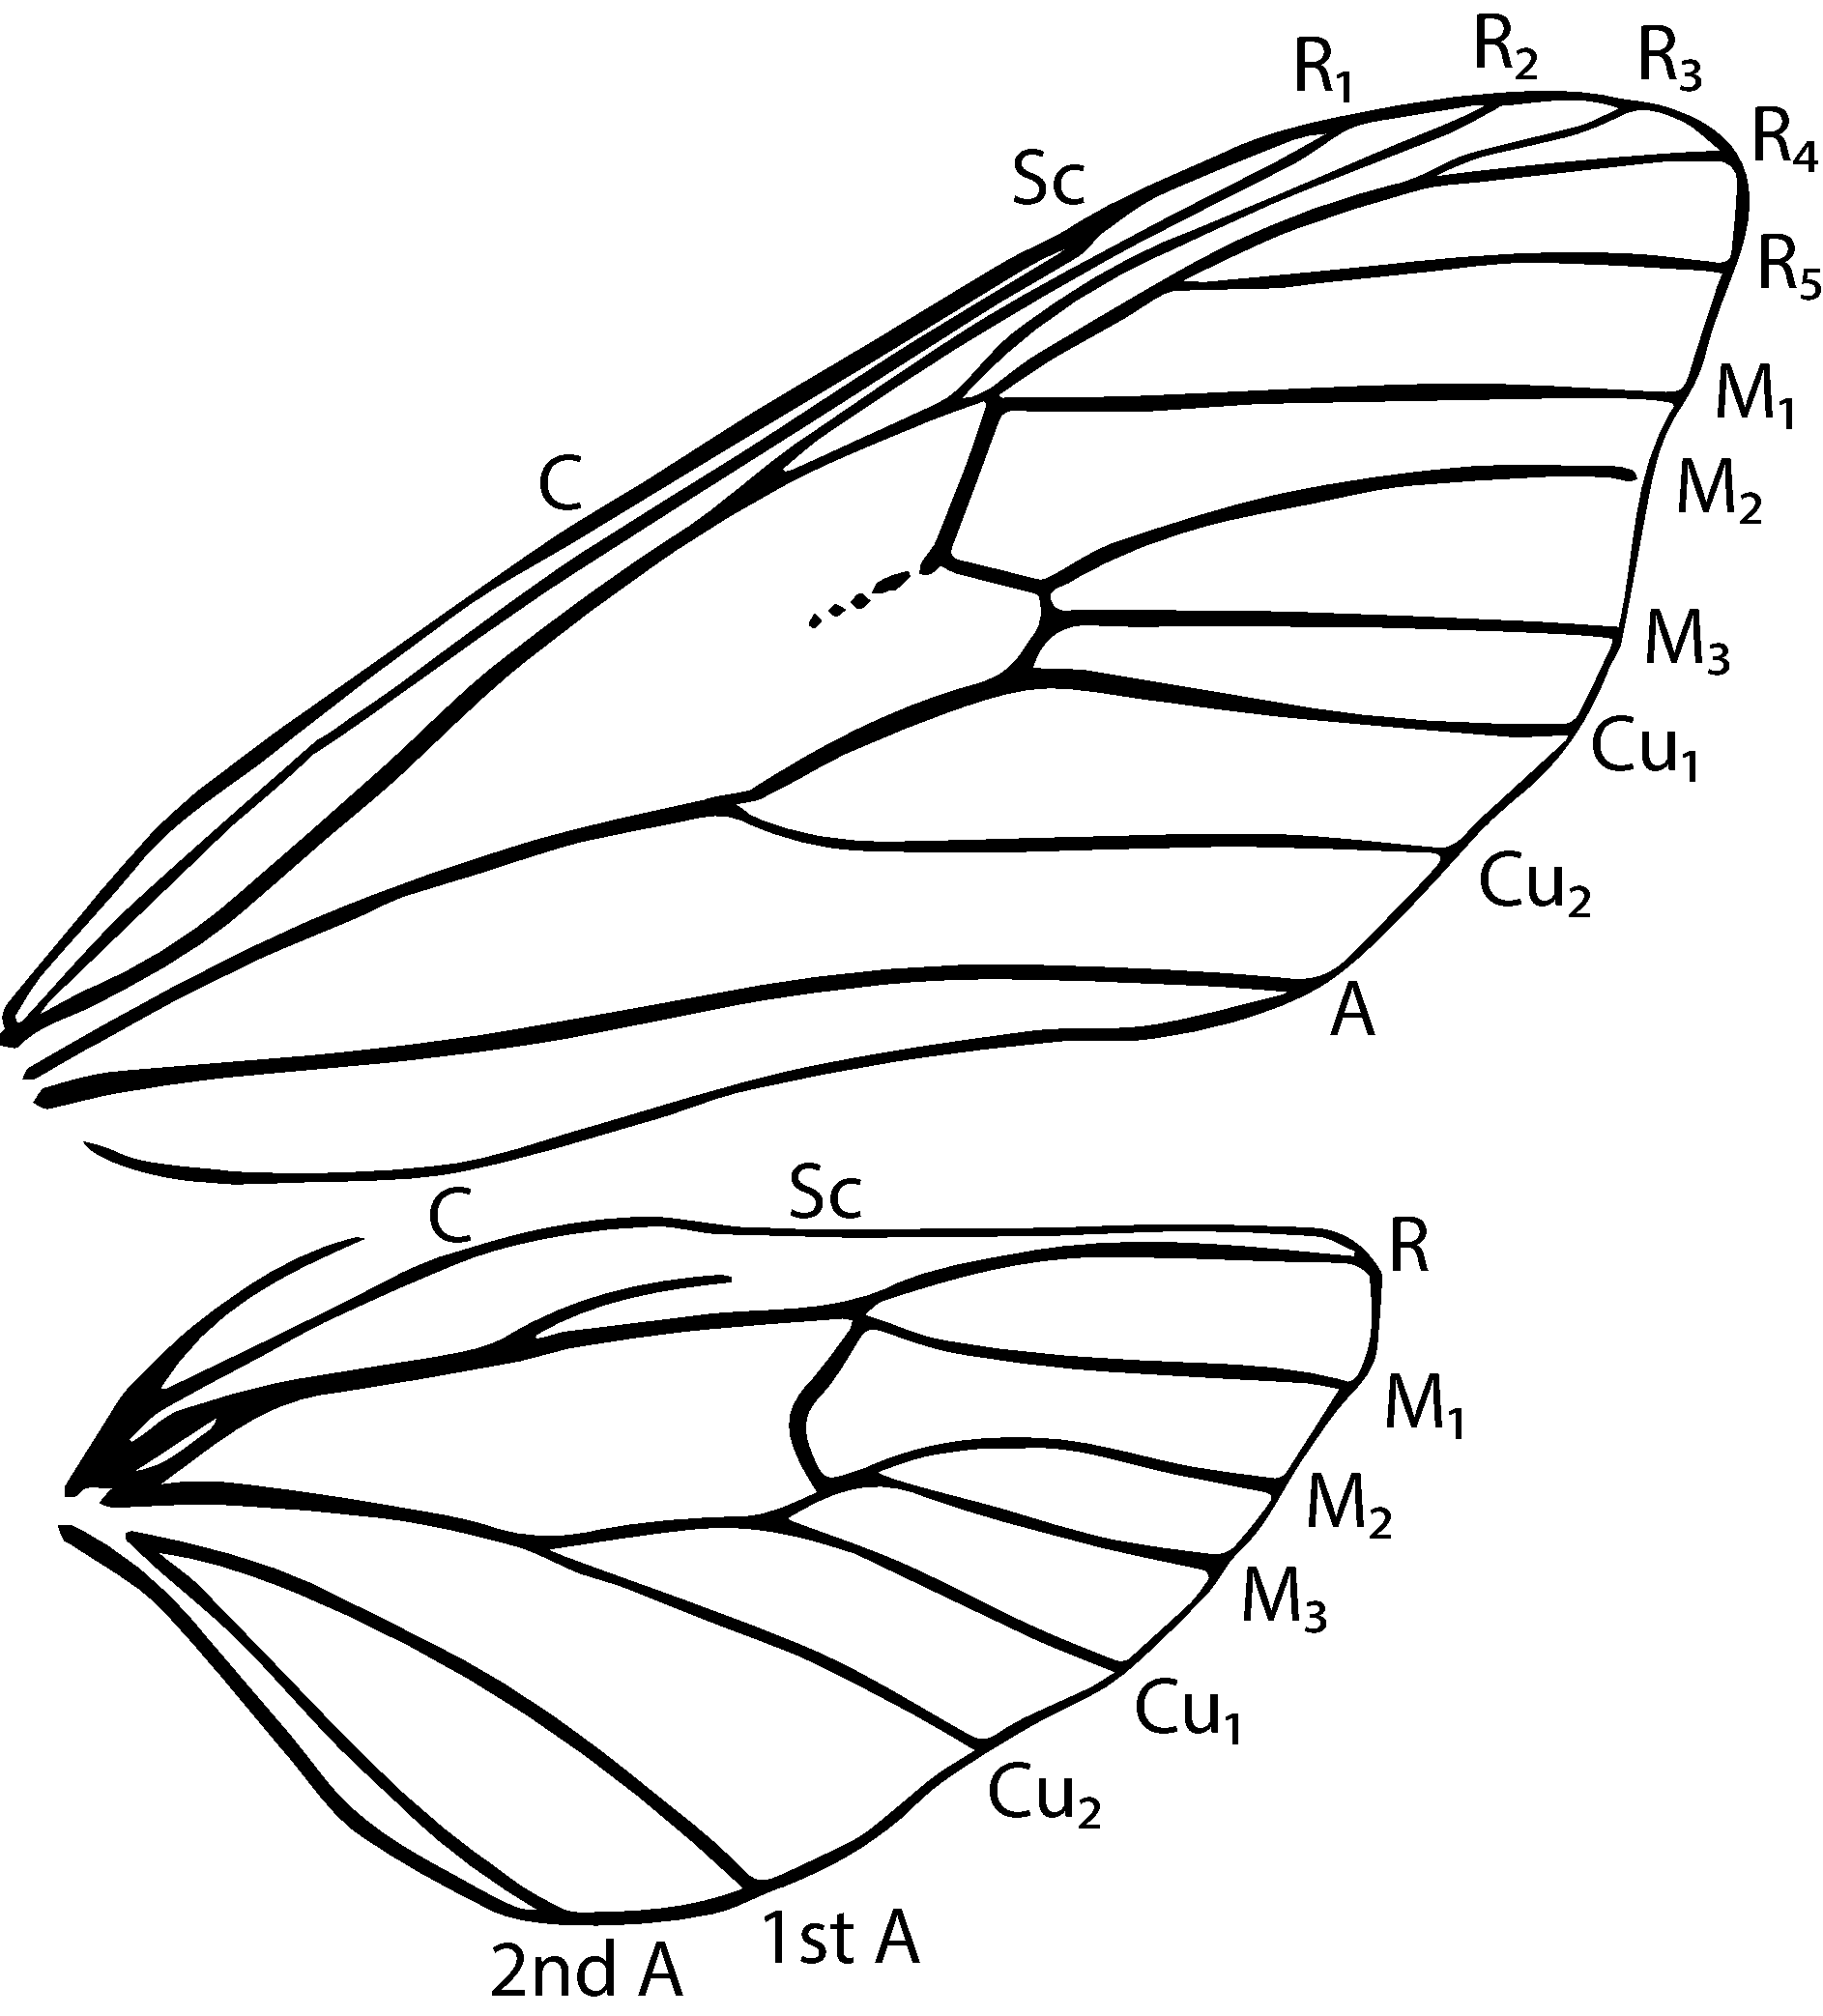
\includegraphics[width=\textwidth]{amphiesmenoptera/ErebidWings}
        \caption{}
        \label{fig:erebid1}
    \end{subfigure}
    \qquad
    \begin{subfigure}[ht!]{0.5\textwidth}
        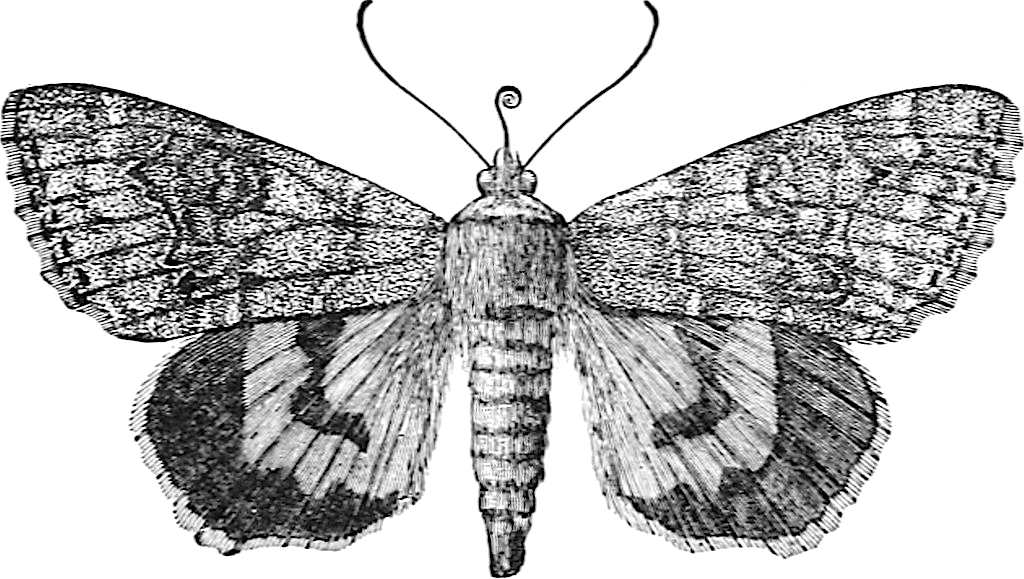
\includegraphics[width=\textwidth]{amphiesmenoptera/catocala}
        \caption{}
        \label{fig:erebid2}
    \end{subfigure}
    \caption{Erebidae. \textbf{(a)} Wings \citep[][Fig. 450]{bhlitem16791elementary}; \textbf{(b)} habitus \citep[Modified from Fig. 53 in][]{bhlitem118262}}\label{fig:erebids}
\end{figure}

\begin{theo}
{}Why are butterflies, which are diurnal, so conspicuous in their coloration, whereas most moths, which are nocturnal, are drab?
\end{theo}

\FloatBarrier
\section{Trichoptera}\label{Trichoptera}\index{Trichoptera}

\noindent{}\textbf{Trichoptera} comprises approximately 13,000 species, the vast majority of which are aquatic as larvae. Larvae exhibit diverse life history strategies and serve as important indicators of environmental health. For these reasons, we'll be examining larval specimens alongside adults. Larvae use silk extensively, often constructing static or portable shelters. Adult mouthparts are diagnostic for the order, being highly reduced (haustellum) but with long palpi.

\subsubsection{Hydroptilidae (micro-caddisflies)}\index{Hydroptilidae}
\noindent{}\textit{Diagnostic characters:} antennae short; mesoscutum without warts; fore tibia with 1 spur; body very small (usually less than 5 mm); usually mottled grayish or brownish and very hairy (figure \ref{fig:hydrop1}).\vspace{3mm}

\noindent{}\textit{Natural history:} These insects are among the smallest trichopterans, rarely measuring \textgreater5 mm as adults. Larvae are free-living until the final instar, which builds a silken structure referred to as a ``purse case'' (figure \ref{fig:hydroptilid2}). Larvae feed on filamentous algae and/or diatoms.

\begin{figure}[ht!]
    \centering
    \begin{subfigure}[ht!]{0.6\textwidth}
        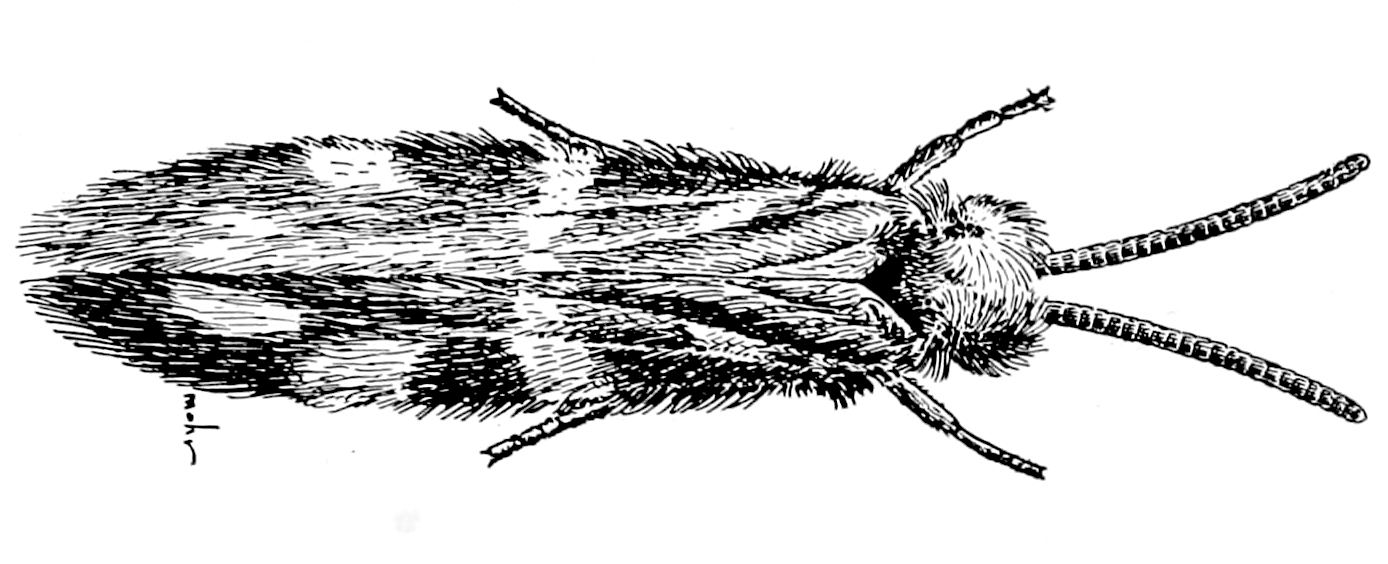
\includegraphics[width=\textwidth]{amphiesmenoptera/hydroptilidHabitus}
        \caption{}
        \label{fig:hydrop1}
    \end{subfigure}
    \hfill
    \begin{subfigure}[ht!]{0.28\textwidth}
        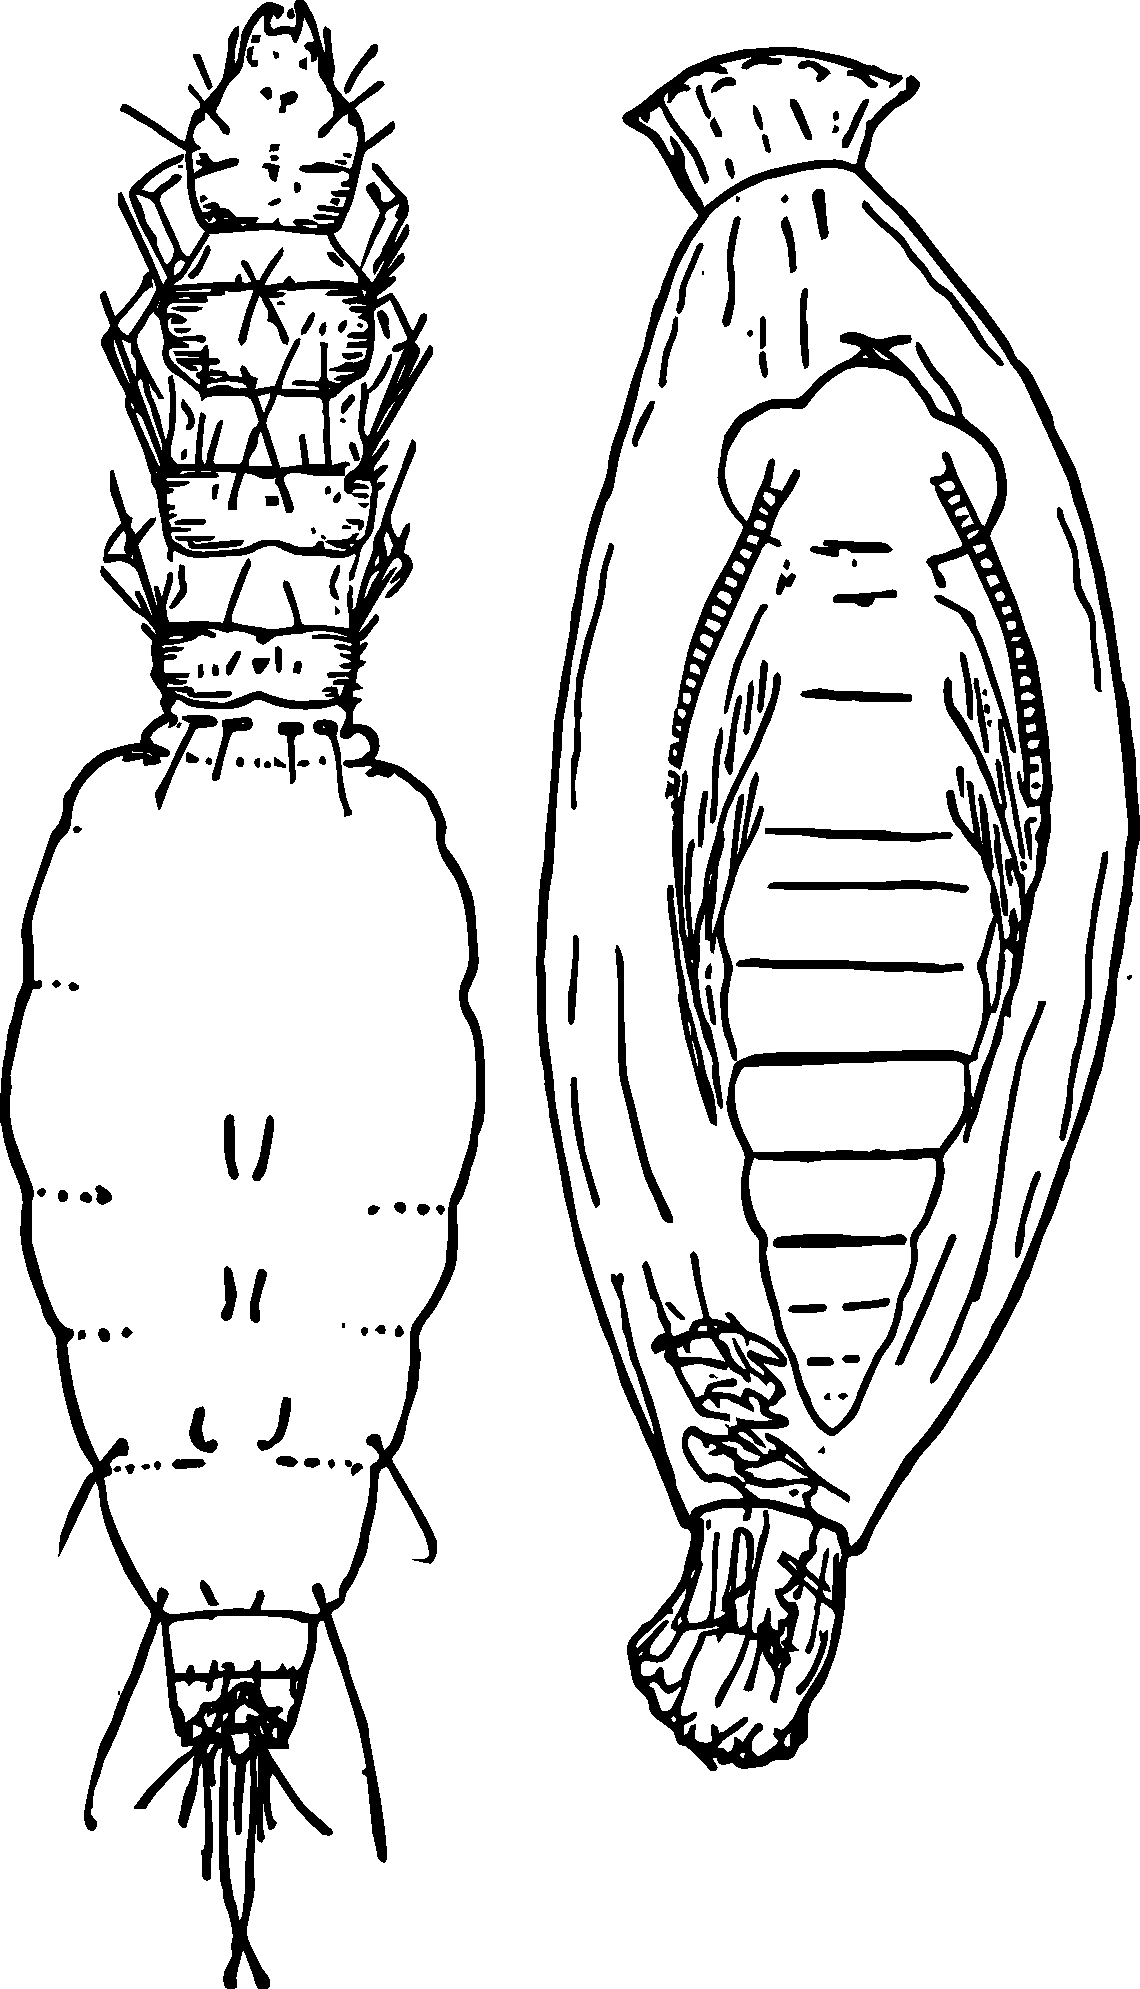
\includegraphics[width=\textwidth]{amphiesmenoptera/hydroptilidaeLarva}
        \caption{}
        \label{fig:hydroptilid2}
    \end{subfigure}
    \caption{Hydroptilidae. \textbf{(a)} Dorsal habitus \citep[modified from Fig. 540 in][]{bhl50956}; \textbf{(b)} larval habitus and pupa \citep[Modified from Fig. 1372 in][]{bhlitem118010freshwater}}\label{fig:hydroptilids}
\end{figure}

\subsubsection{Hydropsychidae (net-spinning caddisflies)}\index{Hydropsychidae}
\noindent{}\textit{Diagnostic characters:} antennae long but usually less than 2$\times$ body; ocelli absent; maxillary palp 5-segmented, with apical segment longer than preceding segments; mesoscutum without warts (Fig. \ref{fig:hydropsychid1}); fore tibia without preapical spurs.\vspace{3mm}

\noindent{}\textit{Natural history:} Larvae (figure \ref{fig:hydropsychid2}) construct trumpet-shaped retreats, attached to rocks in lotic environments. Detritus and invertebrates that get caught in these nets serve as forage for these caddisfly larvae. 

\begin{figure}[ht!]
    \centering
    \begin{subfigure}[ht!]{0.3\textwidth}
        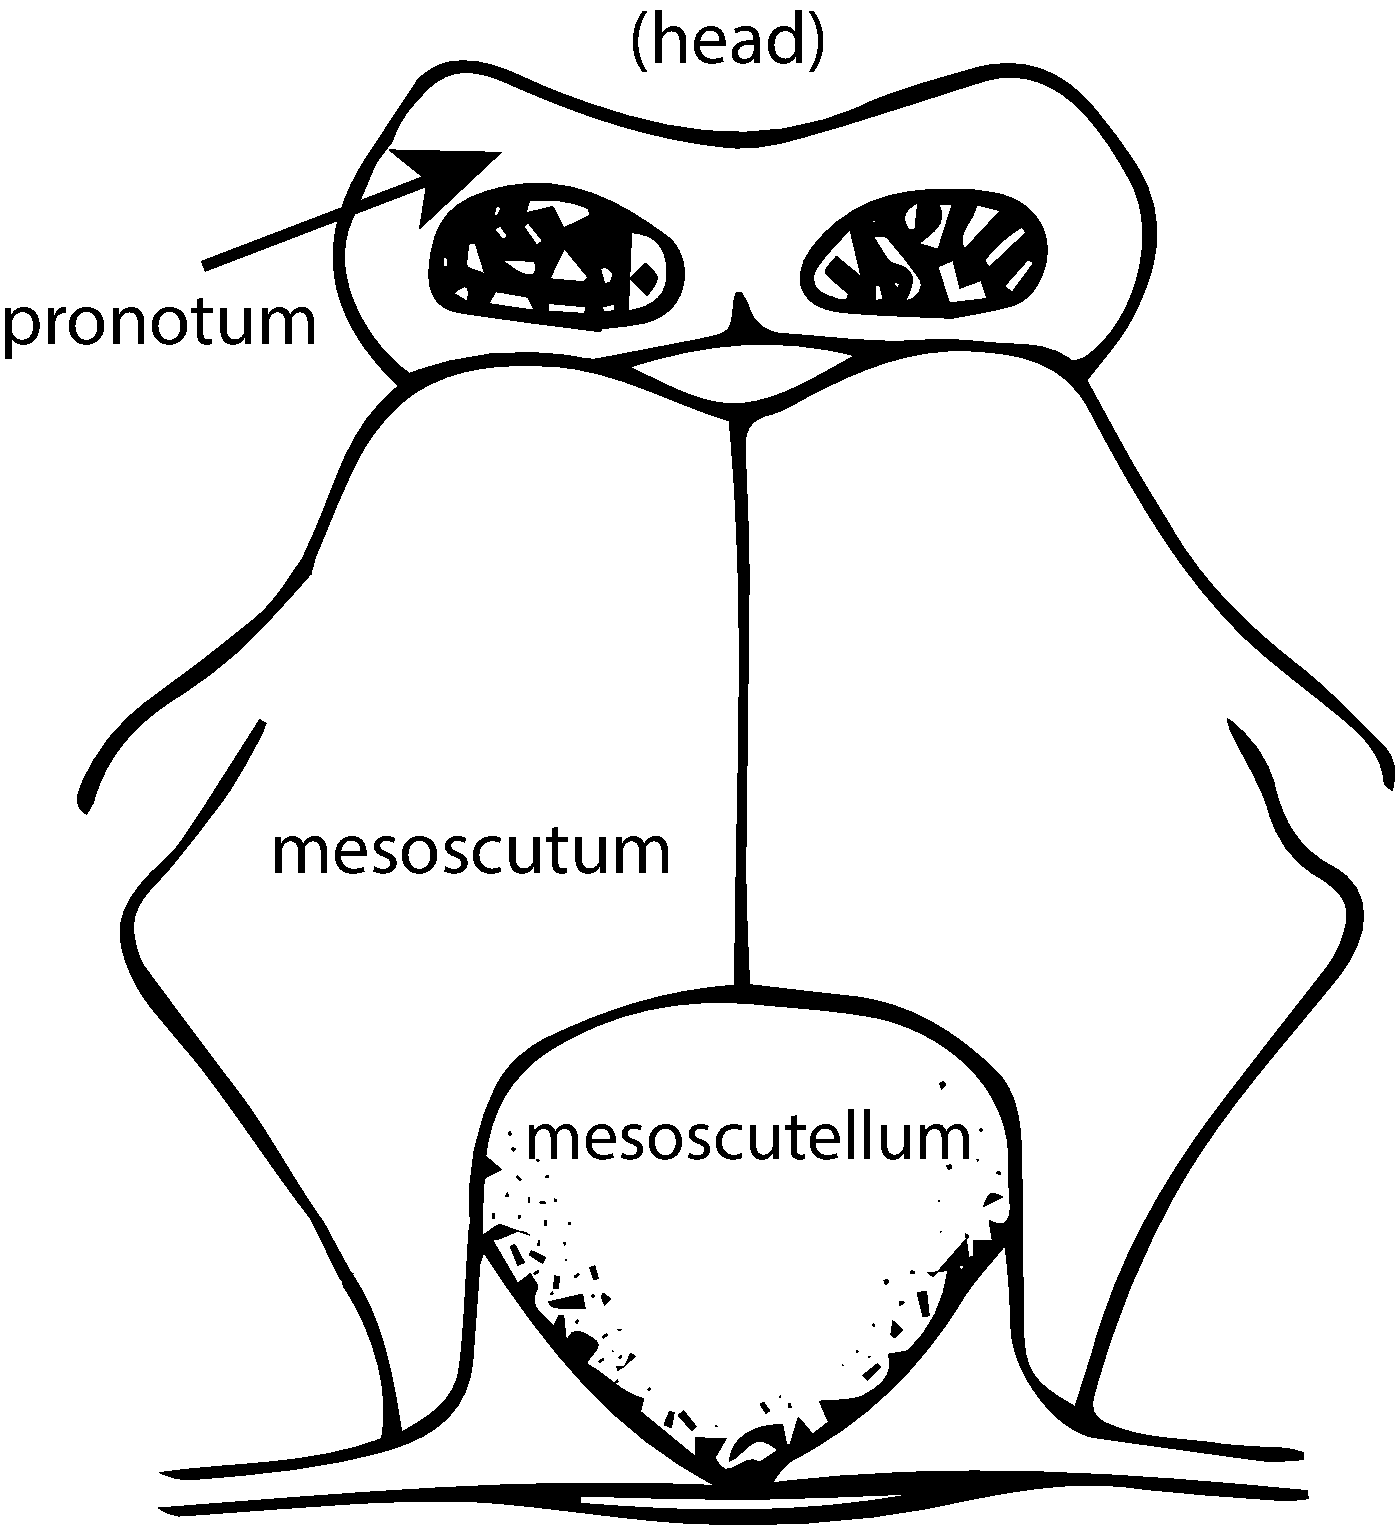
\includegraphics[width=\textwidth]{amphiesmenoptera/TrichoImage03}
        \caption{}
        \label{fig:hydropsychid1}
    \end{subfigure}
    \hfill 
    \begin{subfigure}[ht!]{0.4\textwidth}
        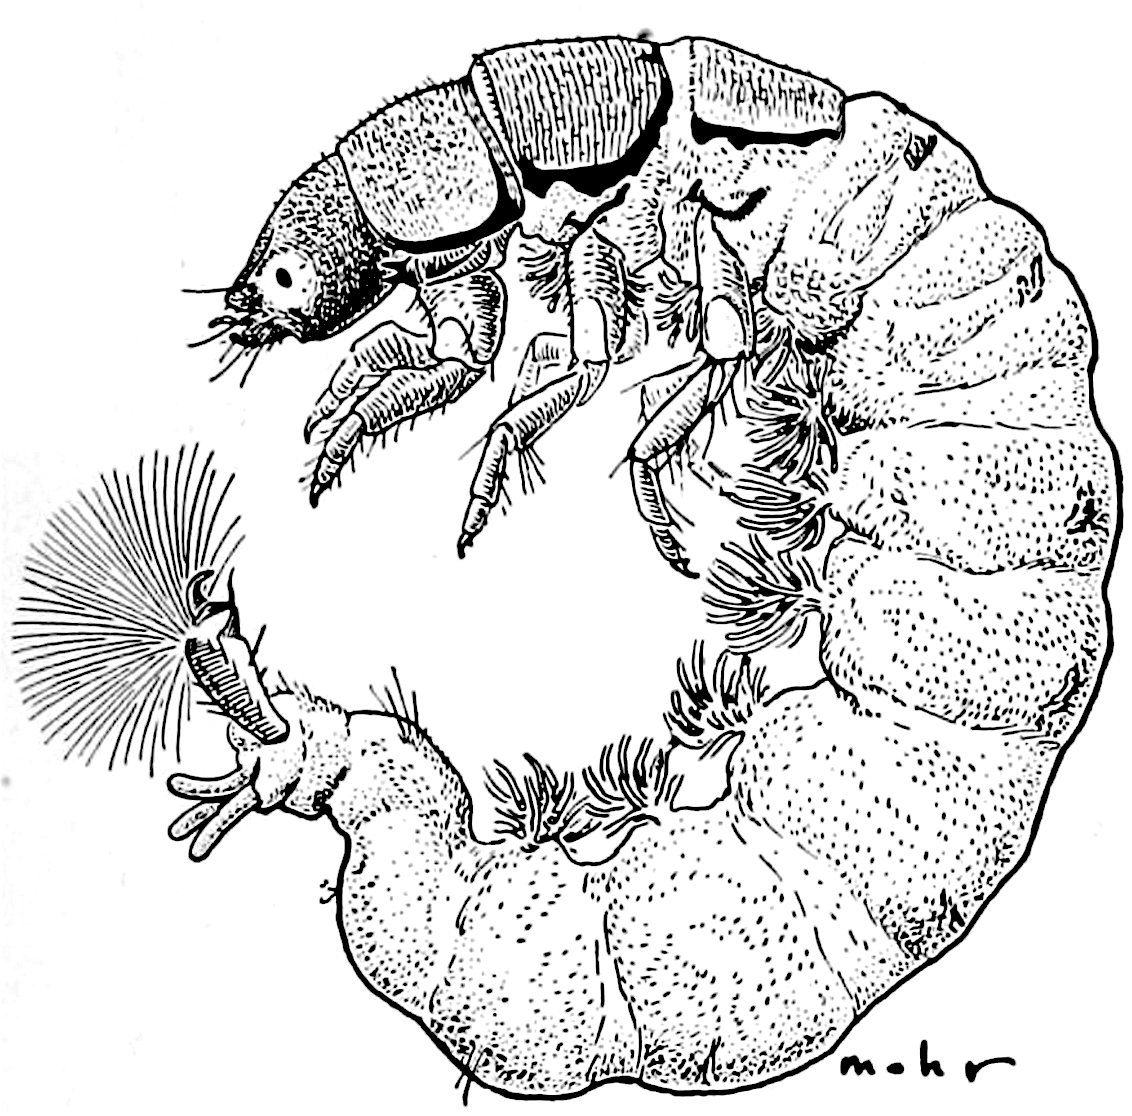
\includegraphics[width=\textwidth]{amphiesmenoptera/HydropsychidLarva}%https://archive.org/stream/bulletin2319441945illi/#page/81/mode/1up
        \caption{}
        \label{fig:hydropsychid2}
    \end{subfigure}
    \caption{Hydropsychidae. \textbf{(a)} Dorsal view of thorax \citep[][Fig. 80]{bhl50956}; \textbf{(b)} larval habitus \citep[][Fig. 281]{bhl50956}}\label{fig:hydropsychids}
\end{figure}

\subsubsection{Leptoceridae (long-horned caddisflies)}\index{Leptoceridae}%http://bmcevolbiol.biomedcentral.com/articles/10.1186/1471-2148-11-10
\noindent{}\textit{Diagnostic characters:} body slender small to medium-sized (5--17 mm); antennae usually 2$\times$ body length (figure \ref{fig:lepto1}); ocelli absent; pronotum with a pair (or 2) of warts separated by notch; dorsal mesoscutum with 2 bands of setiferous punctures instead of setal warts (figure \ref{fig:lepto2}).\vspace{3mm}

\noindent{}\textit{Natural history:} Larvae mostly detritivorous shredders and algae (periphyton) scrapers; some species predators. Larvae, which also have relatively long antennae, typically construct tubular cases.

\begin{figure}[ht!]
    \centering
        \begin{subfigure}[ht!]{0.25\textwidth}
        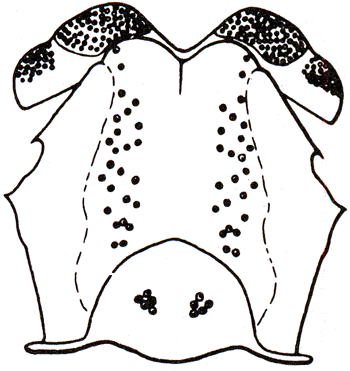
\includegraphics[width=\textwidth]{amphiesmenoptera/TrichoImage07}
        \caption{}
        \label{fig:lepto2}
    \end{subfigure}
   \hfill 
        \begin{subfigure}[ht!]{0.68\textwidth}
        \reflectbox{\includegraphics[width=\textwidth]{amphiesmenoptera/TrichoImage06}}
        \caption{}
        \label{fig:lepto1}
    \end{subfigure}
\caption{Leptoceridae. \textbf{(a)} Dorsal view of thorax \citep[][Fig. 82]{bhl50956}; \textbf{(b)} habitus \citep[][Fig. 863]{bhl50956}}\label{fig:leptoc}
\end{figure}

\subsubsection{Phryganeidae (large caddisflies)}\index{Phryganeidae}
\noindent{}\textit{Diagnostic characters:} Antennae usually about as long as body (figure \ref{fig:phrygan1}); ocelli present; fore tibia with 2 or more spurs; middle tibia with 4 spurs; male maxillary palp 4-segmented (figure \ref{fig:phrygan2}); among the largest caddisflies; often mottled and brown.\vspace{3mm}

\noindent{}\textit{Natural history:} Larvae make portable cases from a diverse array of materials and can usually be found in cold, lentic environments. Larvae are mostly detritivores.

\begin{figure}[ht!]
    \centering
    \begin{subfigure}[ht!]{0.68\textwidth}
        \includegraphics[width=\textwidth]{amphiesmenoptera/PhryganeidHabitus}
        \caption{}
        \label{fig:phrygan1}
    \end{subfigure}
    \hfill
    \begin{subfigure}[ht!]{0.25\textwidth}
        \includegraphics[width=\textwidth]{amphiesmenoptera/TrichoImage01}
        \caption{}
        \label{fig:phrygan2}
    \end{subfigure}
    \caption{Phryganeidae. \textbf{(a)} Habitus \citep[][Fig. 591]{bhl50956}; \textbf{(b)} male maxillary palp \citep[][Fig. 64]{bhl50956}}\label{fig:phrygan}
\end{figure}

\subsubsection{Limnephilidae (northern caddisflies)}\index{Limnephilidae}
\noindent{}\textit{Diagnostic characters:} Antennae usually about as long as body (figure \ref{fig:limnephilid1}); ocelli present; fore tibia with 1 spur or none; middle tibia with 2 or 3 spurs; male maxillary palp 3-segmented (figure \ref{fig:limnephilid2}) and often large; body usually brown with dark markings.\vspace{3mm}

\noindent{}\textit{Natural history:} Larvae make portable cases from a diverse array of materials, and they graze on algae or scavenge. This family also includes some species that are terrestrial.

\begin{figure}[ht!]
    \centering
    \begin{subfigure}[ht!]{0.68\textwidth}
        \reflectbox{\includegraphics[width=\textwidth]{amphiesmenoptera/LimnephilidaeHabitus}}
        \caption{}
        \label{fig:limnephilid1}
    \end{subfigure}
    \hfill
    \begin{subfigure}[ht!]{0.15\textwidth}
        \includegraphics[width=\textwidth]{amphiesmenoptera/LimnephilidHead}
        \caption{}
        \label{fig:limnephilid2}
    \end{subfigure}
    \caption{Limnephilidae. \textbf{(a)} Habitus \citep[Modified from Fig. 641 in][]{bhl50956}; \textbf{(b)} male head \citep[][Fig. 65]{bhl50956}}\label{fig:limnephilids}
\end{figure}

\begin{theo}
{}What is your hypothesis for the function of the wart-like protuberances in caddisfly adults? Think about the biology of the adults, and examine these warts under the microscope.
\end{theo}

\FloatBarrier

\section*{Test yourself}
\noindent{}What factors contribute to the overall diversity of Lepidoptera? Can you describe one or two characteristics that could be key innovations or opportunities?\vspace{3mm}

\noindent{}Can you provide two examples of anti-predator adaptations, related to the wing setae?\vspace{3mm}

\noindent{}What are the precursors of tympana? Do you think the ``ears'' on different body regions in different lepidopterans are homologous?\vspace{3mm} 

\noindent{}What trends do we see across the phylogeny of Lepidoptera, with respect to feeding biology, mouthpart morphology, and wing morphology?\vspace{3mm}

\noindent{}Familiarize yourself with the following taxon names, which refer to organisms you are likely to encounter in the northeastern USA and/or which are phylogenetically relevant. Can you describe how these arthropods live (natural history) and roughly how diverse they are? Do you know how they're related to one another? If you had to choose a family to study from the taxa below which one would it be and why?

\begin{enumerate} 
\item Amphiesmenoptera
\item Ditrysia
\item Rhopalocera
\item Micropterigidae
\item Annulipalpia
\item Integripalpia
\end{enumerate}

\noindent{}Trichoptera is the most diverse aquatic taxon. What factors contribute to their overall diversity, compared to Odonata, Ephemeroptera, and Plecoptera?\vspace{3mm}

\noindent{}Can you describe one or two characteristics that could be key innovations or opportunities for Trichoptera?\vspace{3mm}

\noindent{}With the mouthpart modification we see in Trichoptera, another vital, non-feeding function was lost. Can you describe how trichopterans solve some problems associated with mandible reduction?\vspace{3mm}

\noindent{}What trends do we see across the phylogeny of Trichoptera, with respect to feeding biology and silk use? 

\clearpage
\thispagestyle{empty}